\documentclass[10pt,b5paper,twoside,openright]{book}
%Template for project and MSc project reports created by MSc Morten Fyhn Amundsen
\usepackage{config}
\makeglossaries
\loadglsentries{glossaries}

\begin{document}

\frontmatter
\pagestyle{plain}
\begingroup
\let\cleardoublepage\clearpage
%Problem description - describing the project tasks, supervisor, and co-supervisor - is the first page of the report. For MSc theses, this is generated by the DAIM system. For project reports, you generate this page yourself.
%!TEX root = ../Thesis.tex
\chapter*{\englishproblemname}
\addcontentsline{toc}{chapter}{\englishproblemname}

\textbf{Introduction: }
This project aims to develop a method for multi-agent control of Autonomous Underwater Vehicles (AUVs) by combining the 3D hand position concept with a selected multi-agent control algorithm. The goal is to enable accurate formation control, path following, and collision avoidance for AUVs in a multi-agent system.

\textbf{Objective: }
\begin{itemize}
    \item Perform a literature study on control methods for multi-agent systems with double integrator dynamics, including relevant papers on the 3D hand position concept and multi-agent control algorithms.
    \item Select a suitable multi-agent control algorithm and integrate it with the 3D hand position concept to develop a control strategy for multi-agent control of AUVs.
    \item Develop the theory for the combined control method, including stability analysis.
    \item Conduct simulation studies to validate the effectiveness and performance of the developed control method in formation control, path following, and collision avoidance tasks.
\end{itemize}


\textbf{Expected Outcome: }
The expected outcome of this project is an advanced control method that combines the 3D hand position concept with a selected multi-agent control algorithm to achieve accurate and robust multi-agent control of AUVs. The developed control method will be validated through simulation studies, demonstrating its effectiveness in various scenarios.


\textbf{Conclusion: }
By combining the 3D hand position concept with a selected multi-agent control algorithm, this project aims to provide a novel control method for AUVs in a multi-agent system. The proposed method has the potential to significantly enhance the formation control, path following, and collision avoidance capabilities of AUVs, contributing to advancements in autonomous underwater robotics.


% \textcolor{DarkOrange}{To be formulated thoroughly later.}

% The parts I have addressed so far are marked in bold. I have marked the general multi-agent literature study in italics, as it was partly covered while writing the conference paper.
% \begin{itemize}
%     \item Perform a literature study on control methods of multi-agent systems with double integrator dynamics.
%     \item \textbf{Choose a multi-agent control method that is suitable to combine with the 3D hand position method and merge these, to develop a control method for multi-agent control of AUVs.}
%     \item \textbf{Validate the theoretical results through a simulation study.}
%     \item Validate the theoretical results through high-fidelity simulations/experiments.
%     \item \textit{Do a literature study on multi-agent control methods for marine vehicles (ASVs and AUVs), to put your results into its research context.}
% \end{itemize}
%
\clearpage

%!TEX root = ../Thesis.tex
\chapter*{\englishabstractname}
\addcontentsline{toc}{chapter}{\englishabstractname}
%
This thesis presents a novel control law for formation path following with \glspl{auv} using a second-order \gls{nsb} method. \glspl{auv} pose unique challenges in formation control due to their nonlinear and underactuated nature. This thesis aims to leverage the input-output linearizing hand-position controller to enable the application of formation control methods designed for double-integrator systems, that would otherwise not be applicable to \glspl{auv}.

The main contribution of this work is the extension of the \gls{nsb} method to directly handle the inherent second-order dynamics of \glspl{auv}, addressing the double-integrator nature of the system. By directly accounting for these dynamics, the method eliminates the presence of hidden dynamics from low-level control, encountered in first-order methods. The control algorithm utilizes a hand-position controller that transforms the underactuated six-degrees-of-freedom AUV model into a double-integrator system. The \gls{nsb} method is a behavioral control algorithm that enables the creation of a hierarchy of prioritized tasks. To solve the formation-path-following problem, we create three tasks: collision avoidance, formation keeping, and path following. The second-order formulation enables the expression of all dynamics directly in task space.

The method is initially developed centralized, closely linked to the first-order \gls{nsb} methods in the literature.  However, due to practical limitations in real-world applications, a novel distributed version of the \gls{nsb} algorithm is proposed. This distributed method reformulates the formation-keeping task as a consensus problem, enabling different communication topologies without requiring each vehicle to communicate with all others. The control law leverages techniques from sliding mode control to eliminate errors resulting from non-complete communication graphs.

The closed-loop formation-control and path-following systems are analyzed using Lyapunov theory. The centralized method is shown to give a \gls{usges} system while the decentralized method is shown to provide trajectories that are ultimately bounded to an arbitrarily small set depending on the approximation of the switching term in the sliding mode controller. With an ideal switching controller, the system is shown to be asymptotically stable.

The method's effectiveness is then demonstrated through extensive MATLAB simulation studies. Both the centralized and distributed methods are tested under a range of different scenarios, and the distributed method is compared with existing methods from the literature. The second-order \gls{nsb} method is demonstrated to have lower steady-state errors compared to other methods. The results demonstrate the potential of the second-order \gls{nsb} method for achieving accurate formation control and path following with \glspl{auv}.
%
\clearpage

%!TEX root = ../Thesis.tex
\chapter*{\norwegianabstractname}
\addcontentsline{toc}{chapter}{\norwegianabstractname}
%
Denne oppgaven presenterer en ny styringsmetode for formasjonsbanefølging med autonome undervannsfartøy ved hjelp av en andreordens nullromsbasert atferdsmetode. Autonome undervannsfartøy byr på unike utfordringer innen formasjonsbanefølging på grunn av deres ulineære og underaktuerte natur. Målet med oppgaven er å utnytte inngang-utgang-linearisering ved hjelp av håndposisjonskonseptet for å muliggjøre anvendelse av formasjonsstyringsmetoder som er utviklet for dobbelt-integrator-systemer, som ellers ikke ville vært anvendelige for autonome undervannsfartøy.

Det viktigste bidraget i dette arbeidet er utvidelsen av den nullromsbaserte metoden til å direkte håndtere den iboende andreordens dynamikken til undervannsfartøy gjennom det inngang-utgang lineariserte dobbelt-integrator systemet. Ved å ta hensyn til all dynamikken i oppgaverommet, eliminerer metoden tilstedeværelsen av skjulte dynamikker fra lavnivåkontroll, som man støter på i førsteordens metoder. Styringsmetoden bruker håndposisjonskonseptet for å tranformere den underaktuerte seks-graders-frihet fartøymodellen til et dobbelt-integrator-system. Den nullromsbaserte atferdsmetoden muliggjør opprettelsen av et hierarki av prioriterte oppgaver. For å løse formasjonsbanefølgingsproblemet definerer vi tre oppgaver: kollisjonsungåelse, formasjonsvedlikehold og banefølging. Den andreordens formuleringen av den nullromsbaserte atferdsmetoden muliggjør å uttrykke all dynamikken til systemet direkte i oppgaverommet. 

Først utvikles en sentralisert metode som likner mye på de førsteordens nullromsbaserte metodene som allerede finnes i litteraturen. Deretter, på grunn av praktiske begrensninger i virkelige anvendelser, presenterer vi en ny distribuert versjon av metoden. Denne distribuerte metoden omformulerer formasjonsvedlikeholdsoppgaven som et konsensusproblem, og muliggjør ulike kommunikasjonstopologier uten krav om at hvert fartøy må kommunisere med alle andre. Styringsloven utnytter teknikker fra "sliding mode" regulatorer for å eliminere feil grunnet ukomplett kommunikasjons graf.

Lukket-sløyfe-systemet for formasjonsvedlikehold og banefølging analyseres ved hjelp av Lyapunov-teori. Vi viser at den sentraliserte metoden gir et uniformt semi-globalt asymptotisk stabilt system, mens løsningene til systemet under den desentraliserte metoden er til slutt avgrenset til et vilkårlig lite område avhengig av valg av approksimasjon av det diskontinuerlige leddet i "sliding mode" regulatoren. Med en ideell diskontinuerlig regulator er systemet asymptotisk stabilt.


Metodens effektivitet demonstreres gjennom omfattende simuleringsstudier i MATLAB. Både den sentraliserte og distribuerte metoden testes under ulike scenarioer, og den distribuerte metoden sammenliknes med eksisterende metoder fra litteraturen. Det demonstreres at den andreordens nullromsbaserte atferdsmetoden har lavere feil i likevekt sammenliknet med andre metoder. Resultatene viser potensialet til den andreordens nullromsbaserte metoden for å oppnå nøyaktig formasjonsbanefølging for autonome undervannsfartøy.
%
\clearpage

\tableofcontents \clearpage
\listoftables    \clearpage
\listoffigures   \clearpage
\printglossary[type=\acronymtype] \clearpage
%!TEX root = ../Thesis.tex
\chapter*{\englishprefacename}
\addcontentsline{toc}{chapter}{\englishprefacename}
\vspace{-5mm}
This master’s thesis is submitted as a part of the requirements for the master's
degree at the Department of Engineering Cybernetics at the Norwegian University
of Science and Technology. The work presented in this thesis has been carried out under the supervision of
Prof. Kristin Y. Pettersen and Ph.D. candidate Josef Matou\v{s} at the Department of Engineering Cybernetics, NTNU.


During the project, I have been provided Simulink models for the 6-DOF hand-position controller and the first-order NSB method by Josef Matou\v{s}. The Simulink models as well as the included MATLAB code served as a foundation for the Matlab simulator used in Chapter~\ref{cha:sim_matlab}. The simulator was modified and extended to combine both the centralized and decentralized NSB methods with the hand-position controller.

Unless otherwise stated, all figures and illustrations have been created by the author, however, the SVG object for the yellow AUVs found in several of the figures was provided by Josef Matou\v{s}.

I would like to thank my supervisors Kristin Y. Pettersen and Josef Matou\v{s} for providing advice throughout my thesis. Their expertise and feedback have been instrumental in shaping the direction and quality of this work. I would also like to extend my appreciation to my friends for their support, and encouragement, and for being a source of motivation throughout my academic journey. Their presence and willingness to listen have made the last five years of university truly enjoyable.\\[.5cm]


\hfill {\it Erling Syversveen Lie}\\[-6mm]

\hfill {\it Trondheim, June 2023}\enlargethispage*{\baselineskip}
%
\clearpage


%List of Acronyms, and List of symbols can be useful to include if you have many.
\endgroup

\mainmatter
\pagestyle{headings}

\glsresetall
%!TEX root = ../Thesis.tex
\chapter{Introduction}\label{cha:introduction}
%
This introductory chapter motivates the work by discussing the various applications of cooperating \glspl{auv}. The formation path-following problem is motivated, and limitations posed on existing methods by the nonlinear equations of motion are discussed. The thesis problem is further motivated by briefly discussing the features of the hand-position controller and its possible applications. Then, a literature study on formation control methods for double-integrator systems is presented. These methods are viable candidates to be combined with the hand-position controller. The main contributions are listed and the chapter is concluded with an outline of the rest of the thesis.


\section{Motivation}\label{sec:motivation}
\glspl{auv} have become increasingly important for ocean research and exploration. \glspl{auv} are able to perform tasks in harsh and remote environments that may be too dangerous or difficult for human divers, such as collecting data on ocean temperatures, salinity, and currents, mapping the ocean floor, and conducting underwater inspections for the oil and gas industry. They have also been used for studying marine biology and geosciences \citep{das_data-driven_2015, wynn_autonomous_2014}. The use of \glspl{auv} has the potential to significantly improve our understanding of the ocean and its processes, as well as aid in the development of sustainable ocean practices. Unlike \glspl{rov}, \glspl{auv} are not tethered to the research vessel they are deployed from, which enables opportunities for explorations in areas that were previously inaccessible, such as beneath the ice in polar regions \citep{dowdeswell_autonomous_2008}.

The cooperation of multiple \glspl{auv} can enhance their capabilities and enable them to perform tasks that are difficult or impossible for a single \gls{auv} to accomplish. Cooperation among \glspl{auv} can increase mission efficiency, allows the exploration of larger areas, and provide redundancy in case of system failures. One example is the use of fleets of \glspl{auv} for oceanographic studies as mobile sensor networks \citep{leonard_collective_2007}.  Other applications include the use of multiple \glspl{auv} for the inspection of underwater structures or pipelines, in which each vehicle can be equipped with sensors and work together to cover a larger area more quickly. 

Our work concerns the multi-agent formation path-following problem. The vehicles are controlled to follow a desired path while keeping a predefined formation. The path can be preplanned or it can be provided by a higher-level control layer. Formation path following can be achieved using numerous different control strategies, including leader-follower approaches, where one \gls{auv} acts as a leader and the others follow its trajectory \citep{soorki_robust_2011, cui_leaderfollower_2010, wang_leader-follower_2009}, distributed path-following approaches using consensus algorithms \citep{skjetne_nonlinear_2002,ghabcheloo_coordinated_2006, borhaug_formation_2006}, and behavioral approaches that define the behaviors each \gls{auv} should exhibit to achieve a desired formation \citep{monteiro_dynamical_2002, balch_behavior-based_1998}.

What makes formation path following with \glspl{auv} especially complex compared to ground vehicles are the nonlinear underactuated dynamics. The dynamic constraints must be taken into account when designing formation-control algorithms for the systems to remain stable. The nonlinear and underactuated dynamics make many existing formation-control algorithms developed for other types of vehicles impossible or difficult to apply to \glspl{auv}. A promising approach is to use a hand-position input-output linearizing controller to transform the nonlinear equations into kinematic double-integrator systems \citep{matous_trajectory_2023, paliotta_trajectory_2019}, which may enable the application of a varied number of control strategies that could otherwise not be applied directly to \glspl{auv}. \cite{restrepo_tracking--formation_2022} successfully applied an edge-agreement-based distributed formation control law to 3-\gls{dof} \glspl{asv}, using the hand-position to transfer the \gls{asv} models into linear double-integrator dynamics. In this thesis, we will further explore formation control algorithms for multi-agent systems with double-integrator dynamics. We first present a literature study of control methods and then develop a formation control algorithm for double-integrator systems based on the \gls{nsb} control method.

\vspace*{-3mm}
\section{Literature review}\label{sec:literature_review}
This section presents a literature study on control methods for multi-agent systems with double-integrator dynamics. The methods can be grouped into three main categories: consensus-based methods, rigidity-based methods, and \gls{nsb} methods.

Various consensus algorithms have been proposed to solve the formation-keeping problem in double-integrator systems. The consensus problem is a problem in which multiple agents must coordinate to reach a common value in some information state. The information state can be for instance position, velocity, or a path-progress parameter. The formation path-following problem can be considered a special case of the consensus problem with the following objective:
\begin{equation}
    \lim_{t\rightarrow\infty} \mathbf{p}_i(t) - \mathbf{p}_j(t) - \mathbf{d}_{ij} = \mathbf{0},\quad \lim_{t\rightarrow\infty} \mathbf{v}_i(t) - \mathbf{v}_j(t) = \mathbf{0},
\end{equation}
where $\mathbf{p}_i$ and $\mathbf{v}_i$ are the position and velocity vectors for vehicle $i$ and $d_{ij}$ is the desired relative displacement between vehicle $i$ and $j$. For double-integrator systems, the general consensus controller will take the form
\begin{subequations}\label{eq:first_order_consensus}
\begin{align}
    \dot{\mathbf{p}}_i &= \mathbf{v}_i,\\
    \dot{\mathbf{v}}_i &= \bm{\mu}_i\\
    \bm{\mu}_i &= -k_1 \sum_{j\in\mathcal{N}_i}(\mathbf{p}_i-\mathbf{p}_j - \mathbf{d}_{ij}) -k_2 \sum_{j \in  \mathcal{N}_i}( \mathbf{v}_i - \mathbf{v}_j),
\end{align}
\end{subequations}
where $k_1$ and $k_2$ are constant controller gains and $\mathcal{N}_i$ is the set of all neighboring agents of agent $i$. Specific consensus algorithms can typically take slightly different forms depending on the goal, but will generally keep terms based on the difference in position and velocity with neighboring vehicles. A review of general consensus problems is found in \cite{ren_survey_2005}.

\cite{restrepo_tracking--formation_2022} developed a consensus control law that works directly with \glspl{asv} and \glspl{auv} equipped with the hand-position controller moving in the horizontal plane. It combines techniques from integrator backstepping, \glspl{blf}, and sliding-mode-like switching control. While the paper primarily addresses the tracking of an external target vehicle, it can easily be adapted to track a predefined trajectory using a virtual target. The method can be applied to path following by employing a leader-follower scheme, where the leader controls the progress along the path while the other vehicles act as followers. Moreover, in addition to addressing formation keeping and target tracking, the method explicitly tackles collision avoidance and the maintenance of a maximum communication range. The communication between neighboring agents is assumed to be undirected, allowing bidirectional information flow.\looseness=-1

Other consensus algorithms for control of multi-agent systems subject to double-integrator dynamics share many commonalities with each other. For instance, in \cite{miao_formation_2019}, a consensus algorithm is proposed in which a controller utilizes the gradient of a potential field to maintain communication radius, resembling the concept of \glspl{blf} in \cite{restrepo_tracking--formation_2022}. Despite using different notations, the control methods in both papers exhibit clear similarities. Furthermore, in \cite{montanez-molina_formation_2022}, a consensus algorithm is presented for formations with directed communication, employing a backstepping-like controller. Additionally, \cite{girejko_leader-following_2019} introduces a leader-follower tracking consensus controller with a virtual leader. In \cite{mohammadi_leader-following_2021}, a leader-follower tracking controller is proposed, where positions and velocities of the leader and other agents are estimated instead of being precisely known. Similar to \cite{restrepo_tracking--formation_2022}, a switching controller is applied to handle estimate uncertainties.

A different category of formation control methods is rigidity-based methods. \cite{cai_adaptive_2015} proposed a graph rigidity-based adaptive formation control law for vehicles moving in the plane. The robots' dynamics are modeled using Euler-Lagrange-like equations of motion and simplified using the hand position as the system output. The backstepping-based control law with inter-agent distances as controlled variables ensures asymptotic convergence to the desired formation without global position measurements. The rigid graph theory ensures the uniqueness of the formation shape under distance constraints. Because the method is adaptive, it allows for parametric uncertainty. \cite{li_adaptive_2021} formulate a similar method, but based on a bearing-rigid graph instead of a distance-rigid graph. They argue that bearing-only-based control methods have strong appeal due to the natural connection with vision-based control problems.

A third category of formation-control methods is the \gls{nsb} method. The method has so far been developed for multi-agent control of vehicles following single-integrator dynamics, but, as will be shown throughout this thesis, the method can be modified to work with double-integrator dynamics instead. The method was developed for 3-\gls{dof} \glspl{asv} in \cite{arrichiello_formation_2006}, and has been applied in various other works \citep{pereda_towards_2011, arrichiello_cooperative_2010, eek_formation_2021}. It was extended for \glspl{auv} moving in 6-\gls{dof} in \cite{matous_singularity-free_2022}. The main idea is to formulate a prioritized hierarchy of tasks the vehicle should follow in order to exhibit the desired behavior. The desired velocities generated by the lower-priority tasks are projected into the null space of the higher-priority tasks so that they are only satisfied within the subspace where they do not conflict.

\section{Contributions}\label{sec:contributions}
This thesis presents a novel control method for the formation path-following problem with \glspl{auv}. The main contributions can be summarized as follows:
\begin{itemize}
    \item A literature review on multi-agent control methods for systems following double-integrator dynamics.
    \item An extended second-order \gls{nsb} control method that works directly with double-integrator dynamics.
    \item An extension to the specific behavioral tasks developed in \cite{matous_singularity-free_2022} to work at the acceleration level to be compatible with the second-order \gls{nsb} method.
    \item A closed-loop stability analysis of the joint formation-control and path-following system with the extended \gls{nsb} controller.
    \item A novel approach to reformulating the \gls{nsb} algorithm into a distributed method.
    \item A closed-loop stability analysis of the proposed distributed \gls{nsb} method.
    \item An extensive MATLAB simulation study of the centralized and decentralized second-order \gls{nsb} method.
    \item A submitted conference paper to the 62nd IEEE Conference on Decision and Control with the initial results of the centralized second-order \gls{nsb} method \citep{lie_formation_2023}.
\end{itemize}


In this work, we develop an extended \gls{nsb} method for vehicles with double-integrator dynamics and propose an algorithm that uses a \gls{soclik} equation to control the task variables through acceleration inputs. The procedure is inspired by robotic manipulators, where second-order methods are more common,  due to the inherent second-order dynamics of mechanical systems \citep{siciliano_differential_2009, chiaverini_kinematically_2008}. Although existing \gls{nsb} methods are developed for first-order systems, \gls{auv} dynamics are inherently second-order. Therefore, any first-order solution is necessarily perturbed by the dynamics of the maneuvering controller. In contrast, our formulation handles the second-order dynamics directly in the task space as interpretable spring-damper systems.

We apply the 3D hand position method proposed in \cite{matous_trajectory_2023}, which transforms the underactuated six-degrees-of-freedom \gls{auv} model into a double-integrator system. The transformation enables us to develop the formation-control algorithm for simple kinematic point systems. Subsequently, through the design of specific path-following, formation-keeping, and collision-avoidance tasks, the fleet is controlled to follow a preplanned path in formation while avoiding collisions both within the fleet and with external obstacles. Because our reformulated \gls{nsb} method works directly with the second-order system given by the hand position controller, there is no need to transform desired velocities or accelerations into surge and orientation references, as has been done in previous works. Thus, the complexity level of the control design is reduced.

We review two different methods for compensating for unknown ocean currents. The stability of the system under both ocean current compensation methods is studied when the collision avoidance task is inactive. Two methods for external obstacle avoidance are developed for the double-integrator formulation. The first enables the fleet to avoid obstacles as one unit, keeping formation throughout the avoidance maneuver. In the second method, the vehicles are allowed to break formation in order to avoid collisions.

The \gls{nsb} method is inherently centralized, meaning there must be a central node that communicates and coordinates with all the vehicles in the fleet. We develop a novel decentralized reformulation of the \gls{nsb} algorithm. The key insight lies in reformulating the formation-keeping task as a consensus algorithm. Our resulting distributed method requires inter-vehicle communication of a path progress parameter as well as measurements of relative positions and velocities with neighboring vehicles. The proposed control law uses a sliding mode term in the formation-keeping sub-controller to eliminate formation-keeping errors introduced by the path-following task under non-complete communication graphs.

The closed-loop system is analyzed under both the centralized and the decentralized control law. We demonstrate that the formation-keeping and path-following subsystems can be analyzed independently, and analyze the stability for each of them using Lyapunov theory. The system is shown to be \gls{usges} under the centralized controller, whereas the decentralized controller ensures that the trajectories of the system remain bounded when the sliding-mode controller is approximated with a saturation function. With the ideal switching controller, the system is shown to be asymptotically stable.

We provide an extensive set of MATLAB simulation studies, in which both the centralized and decentralized \gls{nsb} methods are tested under different scenarios. The centralized method is tested with two different obstacle avoidance approaches. The decentralized method is first simulated in a general scenario and then compared to two other existing formation path-following methods from the literature. The MATLAB code for one of the external works was handed to us, while we implemented the other controller ourselves following details in the paper.

\section{Outline}\label{sec:outline}
The report is organized as follows. In Chapter~\ref{cha:vehicle_model}, the mathematical \gls{auv} model is presented, as well as all necessary assumptions. Chapter~\ref{cha:hand_position} presents the 3D hand-position input-output linearization method which transforms the highly non-linear equations of motion of the underactuated vehicles into a double-integrator system in position. Chapter~\ref{cha:formation_path_following} introduces notation, assumptions, and mathematical tools for formation path following of fleets of \glspl{auv}. The chapter introduces the mathematical description of a path as a continuous, differentiable parametric function, and it defines the fleet formation as a set of reference vectors relative to the barycenter of the fleet. The chapter also introduces some simple graph theory, which serves as a basis for the development of the distributed \gls{nsb} method.  In Chapter~\ref{cha:nsp}, background theory for the \gls{nsb} algorithm is presented before the general \gls{nsb} method for second-order systems is developed as a natural extension of the first-order \gls{nsb} method. Chapter~\ref{cha:nsb_tasks} presents the centralized \gls{nsb} method. Collision-avoidance, formation-keeping, and path-following tasks are developed for the second-order formulation so that the task solution provides desired accelerations. Then, modifications to the tasks that enable the fleet to compensate for unknown ocean currents and avoid external obstacles are presented. In Chapter~\ref{cha:closed_loop}, the closed loop properties of the centralized control algorithm presented in Chapter~\ref{cha:nsb_tasks} are studied. In Chapter~\ref{cha:distributed_NSB}, the \gls{nsb} method is modified to work in a distributed setting. The closed-loop stability analysis for this method is provided in Chapter~\ref{cha:distributed_closed_loop}. Both the centralized and decentralized control algorithms are simulated in various configurations in MATLAB \citep{matlab_2022} in Chapter~\ref{cha:sim_matlab}.  Finally, Chapter~\ref{cha:conclusions} presents conclusions and future work.

% %!TEX root = ../Thesis.tex
\chapter{First chapter}\label{cha:first}
This is the first chapter that describes the results of your work, and its contents will depend on the problem description. If a literature review is part of the problem description, than it will be natural to present the literature review in Chapter 2 instead of as part of Chapter 1 Introduction.\\
Make sure throughout the thesis to cite your pre-project report if you include material from this (in addition to declaring this in the Preface). For instance:\\
In this section ... will be presented. The material in this section is from the specialization project Name (20XX) {\it i.e. reference to your pre-project}, and is included for the completeness of the thesis.
% Setup and assumptions
\chapter{Vehicle Model}\label{cha:vehicle_model}
This chapter presents the notation and assumptions for the vehicle models in this work. Because the high-level goal of the thesis is to study multi-agent control algorithms suitable to combine with the 3D hand-position method presented in Chapter~\ref{cha:hand_position}, the assumptions on the vehicle models will be similar to those of the original 3D hand-position paper \citep{matous_trajectory_2023}.

We consider a standard six-degrees-of-freedom \gls{auv} model with an unknown irrotational current. The position of the vehicle in the \gls{ned} coordinate frame is denoted by $\bm{\eta} \in \mathbb{R}^3$, the attitude is parameterized using a rotation matrix $\mathbf{R}\in SO(3)$, and the translational and rotational velocities in the vehicle's body-fixed coordinate frame are denoted by $\bm{\nu}\in\mathbb{R}^3$ and $\bm{\omega}\in\mathbb{R}^3$, respectively. 

The \gls{auv} is affected by an unknown constant irrotational ocean current $\mathbf{v}_c\in\mathbb{R}^3$. We define the relative velocity between the \gls{auv} and the current as $\bm{\nu}_r = \bm{\nu} - R^\mathrm{T}\mathbf{v}_c$, and the concatenated velocity vector as $\bm{\zeta}_r^\mathrm{T} = [\bm{\nu}_r^\mathrm{T},\bm{\omega}^\mathrm{T}]$. The \gls{auv} is subject to external forces and moments due to hydrodynamic forces, gravitational forces, and control inputs. We assume that we can control the surge thrust and torque around all three axes, and denote the control input vector $\mathbf{f} = [T_u,T_p,T_q,T_r]\T$, where $T_u$ is the surge thrust and $T_p,\, T_q, \, T_r$ denote the torques produced by the fins. The \gls{auv} dynamics can be written as follows \citep{fossen_handbook_2021}:
\begin{subequations}\label{eq:auv_model}
\begin{align}
\dot{\bm{\eta}} &= \mathbf{R}\bm{\nu}_r + \mathbf{v}_c, \\
\dot{\mathbf{R}} &= \mathbf{R} \mathbf{S}(\bm{\omega}), \\
\mathbf{M}\dot{\bm{\zeta}_r} + \mathbf{C}(\bm{\zeta}_r)\bm{\zeta}_r + \mathbf{D}(\bm{\zeta}_r)\bm{\zeta}_r + \mathbf{g}(\mathbf{R}) &= \mathbf{Bf},\label{eq:auv_model_c}
\end{align}
\end{subequations}
where $\mathbf{M}\in\mathbb{R}^{6\times 6}$ is the mass and inertia matrix, $\mathbf{C}(\bm{\zeta}_r)\in\mathbb{R}^{6\times 6}$ is the Coriolis and centripetal matrix, $\mathbf{D}(\bm{\zeta}_r)\in\mathbb{R}^{6\times 6}$ is the hydrodynamic damping matrix, $\mathbf{g}(\mathbf{R})\in\mathbb{R}^6$ represents the gravitational and buoyancy forces, $\mathbf{B}\in\mathbb{R}^{4\times 6}$ is the control allocation matrix, %. $\mathbf{S}(\cdot)$ is a skew-symmetrix matrix so that $\mathbf{S}(\bm{\omega})\mathbf{x} = \bm{\omega} \times \mathbf{x}$.
and $\mathbf{S} : \mathbb{R}^3 \mapsto \mathfrak{so}(3)$ is the skew-symmetric matrix operator. Note that for any two vectors $\mathbf{a}, \mathbf{b} \in \mathbb{R}^3$, it follows that $\mathbf{S}(\mathbf{a})\mathbf{b} = \mathbf{a} \times \mathbf{b}$, where $\times$ is the vector cross product.

Next, we present the modeling assumptions.
\begin{assumption}\label{assumption:one}
The vehicle is slender, torpedo-shaped with port-starboard and top-bottom symmetry.
\end{assumption}
\begin{assumption}\label{assumption:two}
    The vehicle is neutrally buoyant, with the \gls{cg} and \gls{cb} on the same vertical axis. The distance from \gls{cb} to \gls{cg} is given by the positive constant $z_{bg}$, meaning the center of gravity is located below the center of buoyancy.
\end{assumption}


\begin{assumption}\label{assumption:three}
    The origin of the body-fixed coordinate frame is located at \textit{neutral point} (also commonly referred to as \gls{pp}) which has relative position $[x_o,\,0,\,0]^T$ from the center of gravity, with $x_o$ such that the actuators produce no sway or heave acceleration. Then, there exist $f_u, \, t_p, \, t_q$, and $t_r$ such that
    \begin{equation}\label{eq:assumption_three}
        \mathbf{M}^{-1}\mathbf{Bf} = [f_u,\, 0,\, 0,\, t_p, \, t_q, \, t_r]^T.
    \end{equation}
\end{assumption}

It was shown in \cite{borhaug_straight_2007} that there exists a coordinate transformation that satisfies \eqref{eq:assumption_three} for a 5-\gls{dof} model satisfying Assumption \ref{assumption:one}. The result is trivially extended to 6-\gls{dof} because roll is decoupled from the other degrees of freedom under Assumption \ref{assumption:one}. The coefficients $\epsilon_1$ and $\epsilon_2$ are defined as
\begin{equation}\label{eq:borhaug_transformation}
    \epsilon_1 \triangleq -\frac{m_{55}b_{23} - m_{25}b_{53}}{m_{22}b_{53} - m_{25}b_{23}}, \quad \epsilon_2 \triangleq -\frac{m_{44}b_{32} - m_{34}b_{42}}{m_{33}b_{42} - m_{34}b_{32}},
\end{equation}
where $m_{ij}$ and $b_{ij}$ are the elements on row i, column j of M and B, respectively. The coordinate transformation matrix to the pivot point from the existing coordinate origin (CO) is then given by the matrix $\mathbf{H}_{PP}$ such that $\bm{\zeta}_r^{PP} = \mathbf{H}_{PP} \bm{\zeta}_r^{CO}$:
\begin{equation}\label{eq:pp_transform_matrix}
    \mathbf{H}_{PP} = \begin{bmatrix}
1 & 0 & 0 & 0 & 0 & 0\\
0 & 1 & 0 & 0 & 0 & -\epsilon_1\\
0 & 0 & 1 & 0 & -\epsilon_2 & 0\\
0 & 0 & 0 & 1 & 0 & 0\\
0 & 0 & 0 & 0 & 1 & 0\\
0 & 0 & 0 & 0 & 0 & 1
    \end{bmatrix}.
\end{equation}
We note that for most cylindrical-shaped \glspl{auv}, $\epsilon_1 = -\epsilon_2$. Then $\mathbf{H}_{PP}$ corresponds to a physical translation of the coordinate origin along the $x$-axis of the ship as detailed in \cite[Appendix C]{fossen_handbook_2021}. The points of interest from Assumption~\ref{assumption:two} and \ref{assumption:three} are illustrated in Figure~\ref{fig:auv_model}.
\begin{figure}[ht]
    \centering
    \def\svgwidth{.5\textwidth}
    \import{figures/illustrations}{auv_with_CG_CB_PP.pdf_tex}
    %\vspace{-1em}
    \caption{Illustration of the \gls{auv} with different points of interest. The marked points are the center of gravity (CG), the center of buoyancy (CB), and the pivot point (PP). The coordinate axes show the orientation of the body-fixed coordinate system, however, the origin would be at the pivot point according to Assumption~\ref{assumption:three}.}
    \label{fig:auv_model}
    %\vspace{-0.3em}
\end{figure}

\begin{assumption}
    The \gls{auv} is operating at sufficiently fast ocean-current relative speeds so that it remains fully controllable.
\end{assumption}
Because the torques are produced by fins attached to the \gls{auv}, the vehicle must maintain a minimum ocean current-relative velocity to remain controllable.

\begin{assumption}\label{assumption:four}
The \gls{auv} is operating at sufficiently slow speeds so that the hydrodynamic damping can be considered linear.
\end{assumption}


The structure of the matrices $\mathbf{M}$, $\mathbf{B}$, and $\mathbf{D}$ under Assumptions \ref{assumption:one}, \ref{assumption:three}, and \ref{assumption:four} are
{\allowdisplaybreaks
\begin{subequations}
    \begin{align}
        \mathbf{M} &= \begin{bmatrix}
        m_{11}& 0& 0& 0& 0& 0\\
        0&  m_{22}& 0& 0& 0& m_{26}\\
        0& 0& m_{33}& 0& m_{35}& 0\\
        0& 0& 0& m_{44}& 0& 0\\
        0& 0& m_{35}& 0& m_{55}& 0\\
        0& m_{26}& 0& 0& 0& m_{66}        
        \end{bmatrix},\\
        \mathbf{B} &= \begin{bmatrix}
            b_{11} & 0 & 0 & 0\\
            0 & 0 & 0 & b_{24}\\
            0 & 0 & b_{33} & 0\\
            0 & b_{42} & 0 & 0\\
            0 & 0 & b_{53} & 0\\
            0 & 0 & 0 & b_{64}\\
        \end{bmatrix},\\
        \mathbf{D} &= \begin{bmatrix}
        d_{11}& 0& 0& 0& 0& 0\\
        0& d_{22}& 0& 0& 0& d_{26}\\
        0& 0& d_{33}& 0& d_{35}& 0\\
        0& 0& 0& d_{44}& 0& 0\\
        0& 0& d_{53}& 0& d_{55}& 0\\
        0& d_{62}& 0& 0& 0& d_{66}        
        \end{bmatrix}.
    \end{align}
\end{subequations}
}
\begin{assumption}\label{assumption:five}
    The effect of gravity and buoyancy on the linear velocities is negligible. 
\end{assumption}

Therefore, under Assumptions \ref{assumption:two} and \ref{assumption:five}, the following approximation 
    \begin{equation}
        \mathbf{M}^{-1}\mathbf{g}(\mathbf{R}) \approx \begin{bmatrix}
            0_3\\
            \mathbf{M}_{22}'(W z_{bg}\mathbf{e}_3\times R^T \mathbf{e}_3)
        \end{bmatrix}
    \end{equation}
can be used to simplify dynamics, where $\mathbf{M}_{22}'$ is the lower right part of $M^{-1}$, and $\mathbf{e}_3 = [0, \, 0,\, 1]^T$ is the third axis unit vector. 

\begin{assumption}
    The full state $\{\bm{\eta},\, \mathbf{R},\, \bm{\zeta}_r\}$ is available for feedback. 
\end{assumption}
We do not consider the state estimation problem and assume that the full state is available for feedback.
\chapter{Hand Position Transformation}\label{cha:hand_position}
This chapter details the hand-position input-output feedback linearization transformation used herein to transform the non-linear underactuated \gls{auv} model \eqref{eq:auv_model} to a double-integrator with a constant ocean-current velocity disturbance.

The hand position concept was first introduced in \cite{pomet_hybrid_1992} to stabilize nonholonomic vehicles with unicycle dynamics. The method was extended to marine vehicles moving in the horizontal plane by \cite{paliotta_trajectory_2019}, which was then used as the basis for a formation control method in \cite{restrepo_tracking--formation_2022}. The method was further extended to 6-\gls{dof} underwater vehicles in \cite{matous_trajectory_2023}. In this chapter, we will present the method as derived for \glspl{auv}.

The linearization involves choosing the hand-position point as the system's output. The hand-position point is located a given distance from the vehicle's pivot point along the $x$-axis. Figure~\ref{fig:hand_illustration} illustrates an \gls{auv} with the center of gravity, pivot point, and hand-position point marked. With reference to the \gls{auv} equations of motion \eqref{eq:auv_model}, the hand-position point is defined in terms of the following change of coordinates:
\begin{subequations}\label{eq:hand_position}
    \begin{align}
        \mathbf{p} &= \bm{\eta} + \mathbf{RL},\\
        \mathbf{v} &= \mathbf{R} \bm{\nu}_r + \mathbf{R}(\bm{\omega}\times \mathbf{L}),
    \end{align}
\end{subequations}
where $\mathbf{L} = [h,0,0]^\mathrm{T}$ and $h>0$ is the hand length.\enlargethispage*{\baselineskip}
\begin{figure}[ht]
    \centering
    \def\svgwidth{.5\textwidth}
    \import{figures/illustrations}{hand_position.pdf_tex}
    %\vspace{-1em}
    \caption{Illustration of the \gls{auv} with different points of interest. The marked points are the center of gravity (CG), pivot point (PP), and hand-position point (HP). Additionally, the hand length $\mathbf{L}$ is marked. The dashed line illustrates the vehicle's center line, which contains all the points of interest.}
    \label{fig:hand_illustration}
    %\vspace{-0.3em}
\end{figure}

To derive the feedback linearized equations of motion, we first introduce some notation. Let
\begin{equation}
    \mathbf{M}^{-1} = \begin{bmatrix}
        \mathbf{M}_{11}^\prime & \mathbf{M}_{12}^\prime\\
        \mathbf{M}_{21}^\prime & \mathbf{M}_{22}^\prime,
    \end{bmatrix}
\end{equation}
and
\begin{equation}
    \begin{bmatrix}
    \mathcal{D}_{\bm{\nu}}\\
    \mathcal{D}_{\bm{\omega}}
    \end{bmatrix} = \mathbf{M}^{-1}\mathbf{D}(\bm{\zeta}_r) \bm{\zeta}_r, \quad \begin{bmatrix}
    \mathcal{C}_{\bm{\nu}}\\
    \mathcal{C}_{\bm{\omega}}
    \end{bmatrix} = \mathbf{M}^{-1}\mathbf{C}(\bm{\zeta}_r)\bm{\zeta}_r.
\end{equation}
Then, we can rewrite \eqref{eq:auv_model_c} in the following form
\begin{subequations}\label{eq:nu_omega_compact}
\begin{align}
    \dot{\bm{\nu}}_r &= [f_u,0,0]\T - \mathcal{D}_{\bm{\nu}}(\bm{\zeta}_r) - \mathcal{C}_{\bm{\nu}}(\bm{\zeta}_r),\\
    \dot{\bm{\omega}} &= [t_p,t_q,t_r]\T - \mathcal{D}_{\bm{\omega}}(\bm{\zeta}_r) - \mathcal{C}_{\bm{\omega}}(\bm{\zeta}_r) - \mathbf{M}_{22}^\prime\left(W z_{bg} \mathbf{e}_3 \times R\T e_3\right).
\end{align}
\end{subequations}

Differentiating \eqref{eq:hand_position} with respect to time and inserting for \eqref{eq:nu_omega_compact} yields:
\begin{subequations}\label{eq:output_dynamics}
\begin{align}
    \dot{\mathbf{p}} &= \mathbf{v} + \mathbf{v}_c,\\
    \begin{split}
    \dot{\mathbf{v}} &= \mathbf{R}\left(\dot{\bm{\nu}}_r +\bm{\omega}\times \bm{\nu}_r + \dot{\bm{\omega}}\times \mathbf{L} +  \bm{\omega}\times (\bm{\omega}\times \mathbf{L})\right),\\ 
    &=\mathbf{R}\biggl([f_u,h t_r, -h t_q]\T - \mathcal{D}_{\bm{\nu}}(\bm{\zeta}_r) - \mathcal{C}_{\bm{\nu}}(\bm{\zeta}_r) + \bm{\omega}\times\bm{\nu}_r \\ 
    & \quad + \mathbf{L}\times \left(\mathcal{D}_{\bm{\omega}}(\bm{\zeta}_r) + \mathcal{C}_{\bm{\omega}}(\bm{\zeta}_r) + \mathbf{M}_{22}^\prime\left(W z_{bg} \mathbf{e}_3 \times R\T e_3\right)\right) + \bm{\omega}\times (\bm{\omega}\times \mathbf{L})\biggr).
    \end{split}
\end{align}
\end{subequations}
We note that $\dot{\mathbf{v}}$ is independent of the roll torque $t_p$. Therefore, $t_p$ is used independently to stabilize the roll dynamics by canceling the Coriolis effect
\begin{align}
        t_p &= \mathbf{e}_1\T \mathcal{C}_{\bm{\omega}}(\bm{\zeta}_r). \label{eq:roll_torque}
\end{align}

The following change of input linearizes the output dynamics \eqref{eq:output_dynamics}:
\begin{equation}
    \begin{split}
        \begin{bmatrix}
            f_u \\ t_q \\ t_r
        \end{bmatrix}
        &
        =
        \begin{bmatrix}
            1 & 0 & 0 \\ 0 & 0 & -\frac{1}{h} \\ 0 & \frac{1}{h} & 0
        \end{bmatrix}
        \Big(\mathbf{R}\T\bm{\mu} + \mathcal{D}_{\bm{\nu}}(\bm{\zeta}_r) + \mathcal{C}_{\bm{\nu}}(\bm{\zeta}_r) - \bm{\omega} \times \bm{\nu}_r  \\
        &\quad - \mathbf{L} \times \left(\mathcal{D}_{\bm{\omega}}(\bm{\zeta}_r) + \mathcal{C}_{\bm{\omega}}(\bm{\zeta}_r) + \mathbf{M}_{22}^{\prime}\left(Wz_{bg} \mathbf{e}_3 \times \mathbf{R}\T \mathbf{e}_3\right)\right) \\
        &\quad - \bm{\omega} \times \left(\bm{\omega} \times \mathbf{L}\right)\Big),
    \end{split}
\end{equation}
where $\bm{\mu} \in \mathbb{R}^3$ is the new control input. The resulting output feedback linearized system is given by:\enlargethispage*{2\baselineskip}
\begin{subequations}\label{eq:hand_linearized_system}
    \begin{align}
        \dot{\mathbf{p}} &= \mathbf{v} + \mathbf{v}_c,\\\label{eq:hand_pos_first_derivative}
        \dot{\mathbf{v}} &= \bm{\mu},\\
        \dot{\mathbf{R}} &=  \mathbf{R} \mathbf{S}(\bm{\omega}),\\
        \begin{split}
        \dot{\bm{\omega}} &= \mathbf{f}_0(\bm{\mu}, \bm{\omega}, \mathbf{R}, \mathbf{v})\\
        &= \widebar{\mathbf{L}} \times \left (\mathbf{R}^T\bm{\mu} + \mathcal{D}_{\bm{\nu}} (\bm{\zeta}_r) + \mathcal{C}_{\bm{\nu}} (\bm{\zeta}_r) - \bm{\omega} \times \mathbf{R}^T \mathbf{v}\right )\\
        &\hphantom{=}- \left(\mathbf{\widebar{L}L}^T\right)\left(\mathcal{D}_{\bm{\omega}} (\bm{\zeta}_r) + \mathbf{M}_{22}' (W \mathbf{z}_{gb}\mathbf{e}_3 \times \mathbf{R}^T \mathbf{e}_3)\right), \label{eq:internal_dynamics}           
        \end{split}
    \end{align}
\end{subequations}
where $\widebar{\mathbf{L}} = [1/h,\, 0,\, 0]^T$, $[\mathbf{p}, \mathbf{v}]^\mathrm{T}$ is the external part of the system and $[\mathbf{R}, \,\bm{\omega}]^\mathrm{T}$ is the internal part. The dynamics of the external part of the system are linear, with the ocean current as an unknown disturbance. Because the internal dynamics \eqref{eq:internal_dynamics} are affected by the input $\bm{\mu}$, the internal stability properties of $\mathbf{R}$ and $\bm{\omega}$ must be verified for the specific choice of control law for $\bm{\mu}$.

\chapter{Formation Path-Following}\label{cha:formation_path_following}

The main objective of this work is to study control methods for multi-agent systems. Specifically, the work herein aims to examine existing methods and develop new methods for the formation path following of fleets of \glspl{auv}. This chapter will introduce the necessary assumptions for the paths, the relevant coordinate frames, and the notation used herein to describe fleets of \glspl{auv}.


\section{Equations of motion and coordinate frames}
We consider a fleet of $n$ \glspl{auv} equipped with output-feedback-linearization hand-position controllers. Each vehicle follows the equations of motion \eqref{eq:hand_linearized_system}. We define the stacked position, velocity, and control input vectors of the fleet $\mathbf{p} = [\mathbf{p}_{1}\T, \, \ldots,\, \mathbf{p}_{n}\T]\T$, $\mathbf{v} = [\mathbf{v}_{1}\T, \, \ldots,\, \mathbf{v}_{n}\T]\T$, and $\bm{\mu} = [\bm{\mu}_1\T, \, \ldots,\, \bm{\mu}_n\T]\T$, respectively. We also define the stacked ocean current vector $\mathbf{V}_c = \mathbf{1}_{n,1} \otimes \mathbf{v}_c$, where $\mathbf{1}_{n,1}$ is an $n$-dimensional vector of ones, and $\otimes$ is the Kronecker product. The translational motion of the whole fleet can then be described in terms of the stacked variables
\begin{subequations}\label{eq:fleet_equation}
\begin{align}
    \dot{\mathbf{p}} &= \mathbf{v} + \mathbf{V}_c,\\
    \dot{\mathbf{v}} &= \bm{\mu}.
\end{align}
\end{subequations}

The formation path-following objective will involve controlling the barycenter $\mathbf{p}_b$ of the fleet to follow a predetermined path. The barycenter is defined as follows:
\begin{equation}\label{eq:barycenter}
    \mathbf{p}_b = \frac{1}{n}\sum_{i=1}^n \mathbf{p}_i.
\end{equation}

We let the path be given by a continuous parametric function $\mathbf{p}_p (\xi) : \mathbb{R} \mapsto \mathbb{R}^3$. The path is assumed to be smooth and regular, meaning that it is infinitely differentiable and the partial derivative with respect to $\xi$ satisfies $\left\|\frac{\partial \mathbf{p}_p(\xi)}{\partial \xi}\right\| \neq 0$.

For every point $\mathbf{p}_p(\xi)$, there exists a path-tangential coordinate frame with a corresponding rotation matrix $\mathbf{R}_p$. The path-following error $\mathbf{p}_b^p$ is defined in terms of the barycenter of the fleet in the path-tangential coordinate frame:
\begin{equation}\label{eq:barycenter_path_tangential}
    \mathbf{p}_b^p = \mathbf{R}_p\T\left(\mathbf{p}_b - \mathbf{p}_p(\xi)\right).
\end{equation}

The formation is defined in the formation-centered coordinate frame, centered at $\mathbf{p}_b$ with the same orientation as the path-tangential frame. The position of a vehicle in the formation-centered frame is given by
\begin{equation}\label{eq:formation_centered_frame}
    \mathbf{p}_i^f = \mathbf{R}_p\T \left(\mathbf{p}_i - \mathbf{p}_b \right),
\end{equation}
and the desired positions are given by $\mathbf{p}_{f,1}^f, \ldots, \mathbf{p}_{f,n}^f$. By definition of $\mathbf{p}_b$, the following constraint always holds
\begin{equation}\label{eq:pf_constraint}
    \sum_{i=1}^n \mathbf{p}_i^f = \mathbf{0}.
\end{equation} 
Consequently, $n-1$ desired barycenter-relative positions $\mathbf{p}_{f,i}^f$ are sufficient to uniquely specify the formation, because the final vehicle's position is implied by \eqref{eq:pf_constraint}. The formation is illustrated in Figure~\ref{fig:formation}. 


\begin{figure}[htp]
    \centering
    \def\svgwidth{\textwidth}
    \import{figures/illustrations}{formation_alternative.pdf_tex}
    %\vspace{-1em}
    \caption{Definition of the formation. $\mathbf{O}^f$ denotes the origin of the formation-centered coordinate frame, $\mathbf{O}^p$ denotes the origin of the path-tangential frame and $\mathbf{O}^{NED}$ denotes the origin of the inertial \gls{ned} frame, $\mathbf{p}_i$ denotes vehicle $i$, and $\mathbf{p}_{f,i}^f$ denotes the desired position of vehicle $i$ relative to $\mathbf{p}_b$. Figure inspired by \cite{matous_singularity-free_2022}.}
    \label{fig:formation}
    %\vspace{-0.3em}
\end{figure}

\section{Communication and graph theory}\label{sec:graph_theory}
In this work, both centralized and decentralized methods are presented. Centralized methods require that each vehicle communicates with every other vehicle and the full state of every vehicle is needed for calculation of controller outputs. These methods are typically infeasible to implement in practice because of communication limitations, but they provide interesting theoretical results and may serve as a basis for developing decentralized controllers.

In decentralized methods, each vehicle calculates its own controller output, often with limited knowledge of the state of other vehicles. Each agent may have access to information from only a limited number of local neighbors. This communication topology is represented by a graph, $\mathcal{G} = (\mathcal{V}, \mathcal{E})$, where the set of vertices $\mathcal{V} \coloneqq \{1,2,\ldots,N\}$ corresponds to the agents and the set of edges $\mathcal{E} \subseteq \mathcal{V}^2$ represents the communication between pairs of agents. Let $M$ be the cardinality of $\mathcal{E}$. The set $\mathcal{E}$ is then given by $\{e_k | k = 1, \ldots , M\}$, where each edge $e_k$ is an ordered pair $(i,j) \in \mathcal{E}$ indicating that agent $j$ has access to information from agent $i$. If the graph is \textit{undirected}, information flows in both directions meaning that if a vertex pair $(i,j)\in \mathcal{E}$ then so is $(j,i)$. The graph is \textit{connected} if there exists a path connecting every agent to every other agent, and it is \textit{complete} (fully connected) if there exists an edge between every pair of agents. We let the set of neighbors of a vertex $i$ be denoted by the set
\begin{equation}
    \mathcal{N}_i = \left\{ j \in \mathcal{V} \colon (i,j) \in \mathcal{E}\right\}.
\end{equation}
The Laplacian matrix of the graph is a matrix $\mathbf{L}\in \mathbb{R}^{N\times N}$ such that
\begin{equation}\label{eq:laplacian_matrix}
\mathbf{L}_{ij}=\begin{cases}\sum\limits_{j=1}^{N}a_{ij}, & i=j.\\ -a_{ij}, & i\neq j,\end{cases}, \quad  a_{ij}=\begin{cases} 1, & \mathrm{i}\mathrm{f} \ (j, i)\in \mathcal{E},\\ 0, & \text{otherwise}.\end{cases}
\end{equation}
It is useful in multiple formation-control methods, particularly consensus methods such as the formation-keeping task in our distributed \gls{nsb} method as presented in Chapter~\ref{cha:distributed_NSB}. For an undirected graph, the Laplacian matrix is symmetric positive-semidefinite. It has an eigenvalue $\lambda_0 = 0$ corresponding to the eigenvector $\mathbf{v}_0 = [1,\, \ldots ,\, 1]\T$.\enlargethispage*{\baselineskip}




% Literature review
% \chapter{Consensus algorithms}\label{cha:consensus_algorithms}
\textcolor{DarkOrange}{Entire chapter is to be removed and merged with the literature review and simulation chapters.}
This chapter will introduce consensus algorithms as a solution to formation keeping in multi-agent systems following double-integrator dynamics. The chapter will provide a brief overview of different methods found in the literature detailing differences and similarities. Then, one of the methods is presented in detail. The purpose of the chapter is to present alternative state-of-the-art methods different from the \gls{nsb} method which is the main focus of the rest of the thesis. Furthermore, ideas from the consensus methods presented here will be leveraged to design a distributed \gls{nsb} method later in Section~\ref{sec:distributed_NSB}.


% The methods presented in this chapter are primarily trajectory-tracking methods and not path-following methods, which differ in that the trajectory-tracking problem has time constraints. In contrast, the path-following problem has an extra degree of freedom in the progress rate along the path.

\section{Consensus methods overview}
The consensus problem is a problem in which multiple agents must coordinate to reach a common value in some information state. The information state can be for instance position, velocity, or a path-progress parameter. The formation-path-following can be considered a special case of the consensus problem with the following objective:
\begin{equation}
    \lim_{t\rightarrow\infty} \mathbf{p}_i(t) - \mathbf{p}_j(t) - \mathbf{d}_{ij} = \mathbf{0},\quad \lim_{t\rightarrow\infty} \mathbf{v}_i(t) - \mathbf{v}_j(t) = \mathbf{0}.
\end{equation}
For single integrator systems, the general consensus controller will take the form
\begin{align}\label{eq:first_order_consensus}
    \dot{\mathbf{p}}_i &= \bm{\mu}_i,\\
    \bm{\mu}_i &= -k \sum_{j\in\mathcal{N}_i}(\mathbf{p}_i-\mathbf{p}_j - \mathbf{d}_{ij}),
\end{align}
where $\mathcal{N}_i$ is the set of all neighboring agents of agent $i$. Consensus algorithms for double-integrator can be designed in many different ways, but typically contain terms that are similar to \eqref{eq:first_order_consensus}. A review of general consensus problems is found in \cite{ren_survey_2005}.

The following sections primarily review the formation-keeping and trajectory-tracking method developed by \cite{restrepo_tracking--formation_2022}. The control law was developed directly to work with \glspl{asv} and \glspl{auv} equipped with the hand-position controller moving in the horizontal plane. It combines techniques from integrator backstepping, \gls{blf}, and sliding-mode-like switching control. While the paper primarily addresses the tracking of an external target vehicle, it can easily be adapted to track a predefined trajectory using a virtual target. The method can be applied to path-following by employing a leader-follower scheme, where the leader controls the progress along the path while the other vehicles act as followers. Moreover, in addition to addressing formation keeping and target tracking, the method explicitly tackles collision avoidance and the maintenance of a maximum communication range. The communication between neighboring agents is assumed to be undirected, allowing bidirectional information flow.

We observe that the literature includes other consensus algorithms for multi-agent control of double-integrator dynamics. For instance, in \cite{miao_formation_2019}, a consensus algorithm is proposed where a controller utilizes the gradient of a potential field to maintain communication radius, resembling the concept of \gls{blf} in \cite{restrepo_tracking--formation_2022}. Despite using different notations, the control methods in both papers exhibit clear similarities. Furthermore, in \cite{montanez-molina_formation_2022}, a consensus algorithm is presented for formations with directed communication, employing a backstepping-like controller. Additionally, \cite{girejko_leader-following_2019} introduces a leader-follower tracking consensus controller with a virtual leader. In \cite{mohammadi_leader-following_2021}, a leader-follower tracking controller is proposed, where positions and velocities of the leader and other agents are estimated instead of being precisely known. Similar to \cite{restrepo_tracking--formation_2022}, a switching controller is applied to handle estimate uncertainties.


All the mentioned works share commonalities in their consensus-based controllers. Therefore, we focus on providing a detailed exposition of the controller proposed by \cite{restrepo_tracking--formation_2022}. This particular controller stands out as it has been explicitly validated to be compatible with the hand-position controller and uniquely integrates three crucial aspects: collision avoidance, maintenance of communication range, and target tracking.

\section{Method details}\label{sec:consensus_method}
It is assumed that each agent only has access to local information from a limited number of neighbors. The communication is described by the connected, undirected graph $\mathcal{G}$ as introduced in Section~\ref{sec:graph_theory}.

The method follows the so-called \textit{edge-agreement} representation. The output state of the system is the set of relative positions
\begin{equation}
    \mathbf{z}_{1k} = \mathbf{p}_i - \mathbf{p}_j \quad \forall k \leq M, \quad (i,j) \in \mathcal{E}.
\end{equation}
Each vehicle is equipped with a hand-position controller, and the dynamics are therefore perturbed by the unknown ocean current $\mathbf{v}_c$
\begin{subequations}
\begin{align}
    \dot{\mathbf{p}}_i &= \mathbf{v}_i +\mathbf{v}_c,\\
    \dot{\mathbf{v}}_i &= \bm{\mu}_i.
\end{align}
\end{subequations}

To avoid collisions and maintain communication range, a minimal distance $\delta_k$ and maximal distance $\Delta_k$ are defined for each relative position, yielding the following output constraints
\begin{equation}
    \mathcal{D}_k = \left\{\mathbf{z}_{1k} \in \mathbb  {R}^2 \colon \delta_k < \| \mathbf{z}_{1k} \| < \Delta_k \right\}, \; \forall k \leq M.\label{eq:restrepo_constraints}
\end{equation}

The formation is supposed to track a target also modeled as a double integrator
\begin{align}
    \dot{\mathbf{p}}_o &= \mathbf{v}_o,\\
    \dot{\mathbf{v}}_o &= \bm{\mu}_o.
\end{align}
It is assumed that only the first agent has access to the target's position and velocity, and the tracking error states are defined as
\begin{equation}
    \Tilde{\mathbf{z}}_{1o} \coloneqq \mathbf{p}_i - \mathbf{p}_o - \mathbf{z}_{1o}^d, \quad \mathbf{z}_{2o} \coloneqq \mathbf{v}_1 - \mathbf{v}_0,
\end{equation}
where $\mathbf{z}_{1o}^d$ is the desired displacement. Similarly, the formation error states are defined as
\begin{align}
    \Tilde{\mathbf{z}}_{1k} \coloneqq \mathbf{p}_i - \mathbf{p}_j - \mathbf{z}_{1k}^d, \quad \mathbf{z}_{2k} \coloneqq \mathbf{v}_1 - \mathbf{v}_j, \quad \forall k \leq M.
\end{align}
The full system can be described by the following set of equations
\begin{subequations}
\begin{align}
    \dot{\tilde{\mathbf{z}}}_{1o} &= \mathbf{z}_{2o} + \mathbf{v}_c\label{eq:restrepo_track_error}\\
    \dot{\tilde{\mathbf{z}}}_{1t} &= \mathbf{z}_{2t}\label{eq:restrepo_formation_error}\\
    \dot{\mathbf{z}}_{2o} &= \bm{\mu}_1-\bm{\mu}_o (t)\\
    \dot{\mathbf{z}}_{2t} &= [\mathbf{E}_t\T \otimes \mathbf{I}_2] \bm{\mu}.
\end{align}
\end{subequations}
Here the states $\mathbf{z}_{1t}$ and $\mathbf{z}_{2t}$ are concatenated states corresponding to $N-1$ edges of a spanning tree $\mathcal{G}_t \subseteq \mathcal{G}$. The matrix $\mathbf{E}_t$ represents the incidence matrix of the spanning tree $\mathcal{G}_t$ so that $\mathbf{z}_{1t} =  [\mathbf{E}_t\T \otimes \mathbf{I}_2] \mathbf{p}$. More details on this formulation can be found in \cite{restrepo_tracking--formation_2022}. Since $N$ agents only have $2N$ positional degrees of freedom in the plane, and the tracking error state accounts for $2$ of them, only $N-1$ edges are necessary to fully represent the system state. The remaining edges can be obtained through the linear transform:
\begin{equation}
    \tilde{\mathbf{z}}_1 = [\mathbf{R}\T \otimes \mathbf{I}_2] \tilde{\mathbf{z}}_{1t}, \quad \mathbf{z}_2 = [\mathbf{R}\T \otimes \mathbf{I}_2] \mathbf{z}_{2t},
\end{equation}
where $\mathbf{R}$ is a matrix defined in \cite{restrepo_tracking--formation_2022}.

The control design is based on a backstepping approach. First, a virtual control law for \eqref{eq:restrepo_track_error}-\eqref{eq:restrepo_formation_error} with $\mathbf{z}_{2o}$ and $\mathbf{z}_{2t}$ as inputs is defined. To account for the output constraints $\mathcal{D}_k$ in \eqref{eq:restrepo_constraints}, the virtual controller is designed in terms of the gradient of a \gls{blf}. \glspl{blf} are similar to Lyapunov functions in that they are positive definite, but their domain of definition is restricted to open subsets of the Euclidean space. They grow unbounded as $\mathbf{z}_{1k}$ approaches the boundary of their domain. By ensuring that the \gls{blf} is bounded in the closed loop, it is ensured that the states do not leave the domain of definition. We refer to \cite{tee_barrier_2009} for more details on \glspl{blf}. In this particular case, the domain for the \gls{blf} is defined in terms of the collision avoidance and communication constraints \eqref{eq:restrepo_constraints}:
\begin{equation}
    \mathcal{\Tilde{D}}_k = \left\{\mathbf{\Tilde{z}}_{1k} \in \mathbb  {R}^2 \colon \delta_k < \| \mathbf{\Tilde{z}}_{1k} + \mathbf{z}_{1k}^d \| < \Delta_k \right\}.
\end{equation}
For each $k\leq M$, a candidate \gls{blf} $W_k \colon \mathcal{\Tilde{D}}_k \rightarrow \mathbb{R}_{\geq 0}$ is defined:
\begin{equation}
    W_k(\Tilde{\mathbf{z}}_{1k}) = \frac{1}{2}\left(\|\tilde{\mathbf{z}}_{1k}\| + B_k(\tilde{\mathbf{z}}_{1k}+z_{1k}^d)\right),
\end{equation}
where $B_k(\mathbf{z}_{1k})$ is a non-negative defined in \cite{restrepo_tracking--formation_2022} that satisfies $B_k(\mathbf{z}_{1k}^d) = 0$, $\nabla B_k(\mathbf{z}_{1k}^d) = 0$, and $B_k(\mathbf{z}_{1k}) \rightarrow  \infty$ as either $\|\mathbf{z}_{1k}\| \rightarrow \Delta_k$ or $\|\mathbf{z}_{1k}\| \rightarrow \delta_k$.

The virtual controllers are given by
\begin{subequations}
    \begin{align}
        \mathbf{z}_{2t}^* &= [\mathbf{E}_t\T \otimes \mathbf{I}_2]\mathbf{v}^*,\\
        \mathbf{z}_{2o}^* &= [\mathbf{C}\T \otimes \mathbf{I}_2]\mathbf{v}^*,\\
        \mathbf{v}^* &= -c_1 [\mathbf{E}_t \otimes \mathbf{I}_2]\nabla W(\tilde{\mathbf{z}}_{1t}) - c_1 [\mathbf{C} \otimes \mathbf{I}_2]\tilde{\mathbf{z}}_{1o} - \hat{\mathbf{V}}_c,
    \end{align}
\end{subequations}
where $c_1$ is a positive gain, $\hat{\mathbf{V}}_c$ is a stacked vector of estimates of the ocean current for each agent, and $\mathbf{C} \coloneqq [1\; 0_{1\times(N-1)}]\T$. The following error variables are defined in terms of the virtual controllers: $\tilde{\mathbf{z}}_{2t} = \mathbf{z}_{2t} - \mathbf{z}_{2t}^*$ and $\tilde{\mathbf{z}}_{2o} = \mathbf{z}_{2o} - \mathbf{z}_{2o}^*$.

The total control law is chosen as
\begin{equation}\label{eq:restrepo_controller}
    \begin{split}
        \bm{\mu} = &-c_2 [\mathbf{E}_t \mathbf{R}\mathbf{R}\T \otimes \mathbf{I}_2]\tilde{\mathbf{z}}_{2t} - c_2 [\mathbf{C}\otimes \mathbf{I}_2]\tilde{\mathbf{z}}_{2o} + \dot{\Bar{\mathbf{v}}}^*\\
        &- \gamma \mathrm{sign}\left([\mathbf{E}_t \mathbf{R}\mathbf{R}\T \otimes \mathbf{I}_2]\tilde{\mathbf{z}}_{2t} + [\mathbf{C}\otimes \mathbf{I}_2]\tilde{\mathbf{z}}_{2o}\right),
    \end{split}
\end{equation}
where $c_2, \gamma > 0$ and $\bar{\mathbf{v}}^* = -c_1 [\mathbf{E}_t \otimes \mathbf{I}_2]\nabla W(\tilde{\mathbf{z}}_{1t}) - c_1 [\mathbf{C} \otimes \mathbf{I}_2]\tilde{\mathbf{z}}_{1o}$. The term with the signum function is a sliding-mode-like term that ensures perfect tracking despite the unknown target acceleration $\bm{\mu}_o$. It might be difficult to recognize how this is a consensus algorithm similar to \eqref{eq:first_order_consensus}, however, the control law can be rewritten as 
\begin{equation}
    \begin{split}
        \bm{\mu} = &-c_2 [\mathbf{L} \otimes \mathbf{I}_2](\mathbf{v} - \mathbf{v}^*) - c_2 [\mathbf{C}\otimes \mathbf{I}_2]\tilde{\mathbf{z}}_{2o} + \dot{\Bar{\mathbf{v}}}^*\\
        &- \gamma \mathrm{sign}\left([\mathbf{L} \otimes \mathbf{I}_2](\mathbf{v} - \mathbf{v}^*) + [\mathbf{C}\otimes \mathbf{I}_2]\tilde{\mathbf{z}}_{2o}\right),
    \end{split}
\end{equation}
where $\mathbf{L} = \mathbf{E}_t \mathbf{R} \mathbf{R}\T \mathbf{E}_t\T$ is the Laplacian matrix \eqref{eq:laplacian_matrix} of graph $\mathcal{G}$. One can therefore recognize that each element $\mathbf{u}_i$ in the vector $\mathbf{u} =  -c_2[\mathbf{L} \otimes \mathbf{I}_2](\mathbf{v}-\mathbf{v}^*)$ takes the following form
\begin{equation}
    \mathbf{u}_i = -c_2\sum_{j\in \mathcal{N}_i} (\mathbf{v}_i - \mathbf{v}_j) + c_2\sum_{j\in \mathcal{N}_i} (\mathbf{v}_i^* - \mathbf{v}_j^*),
\end{equation}
which is a consensus term in velocity for each agent similar to \eqref{eq:first_order_consensus}.

\section{Properties and performance}
The algorithm guarantees that the fleet converges to the desired formation and tracks the target without violating collision avoidance and communication range constraints. The method explicitly takes communication limitations into account and allows multiple different communication topologies. The controller \eqref{eq:restrepo_controller} can be implemented in a distributed manner, where each agent only knows the relative position of its neighbors according to the communication graph $\mathcal{G}$.

We implement the control law in the MATLAB simulator detailed in Chapter~\ref{cha:sim_matlab}. The control law \eqref{eq:restrepo_controller} is trivially extended to 3D by replacing all instances of $\mathbf{I}_2$ with $\mathbf{I}_3$ in the Kronecker products. The proof that this works for the external states of the hand-position controller follows directly from \cite{restrepo_tracking--formation_2022}, and the ultimate boundedness of the internal dynamics of the hand-position controller can be derived by combining results from \cite{restrepo_tracking--formation_2022} and \cite{matous_trajectory_2023}. The simulation setup is very similar to that in Section~\ref{sec:general_three_agent}, but there is no external obstacle, and the path parameter is given as a function of time $\xi = t$ to yield a trajectory tracking problem instead of a path-following problem. The fleet is supposed to track a virtual target with a relative displacement specified so the virtual target is at the fleet barycenter. The minimum and maximum distances between vehicles are defined as $\delta = 8 \mathrm{m}$ and $\Delta = 35 \mathrm{m}$.

The initial formation is specified with the vehicles at the opposite side of the fleet center compared to the desired formation. Thus, the collision avoidance performance is tested thoroughly. As can be seen from Figure~\ref{fig:restrepo_relative_distances}, the relative distance between vehicles 2 and 3, denoted by \textit{edge 2} drops below $\delta$. One possible reason for this is that the implemented system uses a smooth approximation to the signum function $\mathrm{sign}(x) = \mathrm{tanh}(\alpha x), \; \alpha >> 0$. Consequently, some of the theoretical guarantees may be lost. Also, simulations with switching behavior are prone to numerical errors. The system was tested with a range of different $\alpha$s with similar results. After the initial constraint violation, the vehicles recover the desired formation, and the formation-keeping error converges to zero as seen in Figure~\ref{fig:restrepo_formation_error}.

Figure~\ref{fig:restrepo_trajectory} shows the trajectory of the fleet. The path is accurately tracked after the initial convergence. The formation remains orthogonal to the \gls{ned}-frame and not the path-tangential frame. This is a natural consequence of only the first vehicle having access to the target vehicle. Furthermore, if the target vehicle is a physical vehicle and not a predefined virtual one, online estimation of the path-tangential frame and its derivatives may be difficult. If the trajectory was accessible to all vehicles instead, it would be possible to modify the algorithm so that the formation is kept relative to the path-tangential frame by specifying $\mathbf{z}_1^d$ as a time-varying function of the trajectory. However, without this limiting assumption, there may also exist other control methods that are better suited.


\begin{figure}[htbp]
    \centering
    \begin{subfigure}[t]{.9\textwidth}
    \centering
    \setlength\figurewidth{.5\linewidth}
    \setlength\figureheight{5.2 cm}
    % This file was created by matlab2tikz.
%
%The latest updates can be retrieved from
%  http://www.mathworks.com/matlabcentral/fileexchange/22022-matlab2tikz-matlab2tikz
%where you can also make suggestions and rate matlab2tikz.
%
\definecolor{mycolor1}{rgb}{0.00000,0.44700,0.74100}%
\definecolor{mycolor2}{rgb}{0.85000,0.32500,0.09800}%
\definecolor{mycolor3}{rgb}{0.92900,0.69400,0.12500}%
%
\begin{tikzpicture}

\begin{axis}[%
unit vector ratio*=1 1 1,
width=0.951\figurewidth,
height=\figureheight,
at={(0\figurewidth,0\figureheight)},
scale only axis,
xmin=-127.596669278219,
xmax=62.5966692782195,
xlabel style={font=\color{white!15!black}},
xlabel={East [m]},
ymin=0,
ymax=150.007326700159,
ylabel style={font=\color{white!15!black}},
ylabel={North [m]},
axis background/.style={fill=white},
title style={font=\bfseries, yshift=-2mm},
title={\textbf{Trajectory}},
axis x line*=bottom,
axis y line*=left,
xmajorgrids,
ymajorgrids,
legend style={legend pos= north west,legend cell align=left, align=left, draw=white!15!black, font=\footnotesize}
]
\addplot [color=mycolor1, line width=1.0pt, mark size=3.5pt, mark=*, mark options={solid, fill=mycolor1, mycolor1}, mark repeat=50]
  table[]{trajectory-1.tsv};
\addlegendentry{Veh. 1}

\addplot [color=mycolor2, line width=1.0pt, mark size=3.5pt, mark=*, mark options={solid, fill=mycolor2, mycolor2}, mark repeat=50]
  table[]{trajectory-2.tsv};
\addlegendentry{Veh. 2}

\addplot [color=mycolor3, line width=1.0pt, mark size=3.5pt, mark=*, mark options={solid, fill=mycolor3, mycolor3}, mark repeat=50]
  table[]{trajectory-3.tsv};
\addlegendentry{Veh. 3}

\addplot [color=black, line width=1.5pt]
  table[]{trajectory-4.tsv};
\addlegendentry{Path}

\addplot [color=black, dotted, line width=0.8pt, forget plot]
  table[]{trajectory-5.tsv};
\addplot [color=black, dotted, line width=0.8pt, forget plot]
  table[]{trajectory-6.tsv};
\addplot [color=black, dotted, line width=0.8pt, forget plot]
  table[]{trajectory-7.tsv};
\addplot [color=black, dotted, line width=0.8pt, forget plot]
  table[]{trajectory-8.tsv};
\addplot [color=black, dotted, line width=0.8pt, forget plot]
  table[]{trajectory-9.tsv};
\addplot [color=black, dotted, line width=0.8pt, forget plot]
  table[]{trajectory-10.tsv};
\addplot [color=black, dotted, line width=0.8pt, forget plot]
  table[]{trajectory-11.tsv};
\addplot [color=black, dotted, line width=0.8pt, forget plot]
  table[]{trajectory-12.tsv};
\addplot [color=black, dotted, line width=0.8pt, forget plot]
  table[]{trajectory-13.tsv};
\addplot [color=black, dotted, line width=0.8pt, forget plot]
  table[]{trajectory-14.tsv};
\addplot [color=black, dotted, line width=0.8pt, forget plot]
  table[]{trajectory-15.tsv};
\addplot [color=black, dotted, line width=0.8pt, forget plot]
  table[]{trajectory-16.tsv};
\addplot [color=black, dotted, line width=0.8pt, forget plot]
  table[]{trajectory-17.tsv};
\addplot [color=black, dotted, line width=0.8pt, forget plot]
  table[]{trajectory-18.tsv};
\addplot [color=black, dotted, line width=0.8pt, forget plot]
  table[]{trajectory-19.tsv};
\addplot [color=black, dotted, line width=0.8pt, forget plot]
  table[]{trajectory-20.tsv};
\addplot [color=black, dotted, line width=0.8pt, forget plot]
  table[]{trajectory-21.tsv};
\addplot [color=black, dotted, line width=0.8pt, forget plot]
  table[]{trajectory-22.tsv};
\addplot [color=black, dotted, line width=0.8pt, forget plot]
  table[]{trajectory-23.tsv};
\addplot [color=black, dotted, line width=0.8pt, forget plot]
  table[]{trajectory-24.tsv};
\end{axis}

\begin{axis}[%
width=1.227\figurewidth,
height=1.227\figureheight,
at={(-0.16\figurewidth,-0.135\figureheight)},
scale only axis,
xmin=0,
xmax=1,
ymin=0,
ymax=1,
axis line style={draw=none},
ticks=none,
axis x line*=bottom,
axis y line*=left
]
\end{axis}
\end{tikzpicture}%
    \vspace*{-2mm}
    \caption{The trajectory of the fleet.}
    \label{fig:restrepo_trajectory}
    \end{subfigure}
    \\
    \begin{subfigure}[t]{.9\textwidth}
    \centering
    \setlength\figurewidth{.8\linewidth}
    \setlength\figureheight{2.1cm}
    \input{tikz_figures/relative_distances}
    \vspace*{-2mm}
    \caption{The relative distances between vehicles. }
    \label{fig:restrepo_relative_distances}
    \end{subfigure}
    \\
    \begin{subfigure}[t]{.9\textwidth}
    \centering
    \setlength\figurewidth{.8\linewidth}
    \setlength\figureheight{2.1cm}
    \input{tikz_figures/formation_error}
    \vspace*{-2mm}
    \caption{The formation error norms.}
    \label{fig:restrepo_formation_error}
    \end{subfigure}
    \vspace*{-2mm}
    \caption{Simulation results for the edge-agreement-based formation control algorithm.}
    \label{fig:sim_results_restrepo}
\end{figure}

Except for the constraint violation, the simulation results look promising as the fleet converges to the formation and tracks the target. However, further inspection shows that the controller commands unphysical actuation. Figure~\ref{fig:restrepo_surge_thrust} shows that the commanded surge thrust peaks at $1000 \, \mathrm{N}$ and goes negative for some vehicles.  As seen in Figure~\ref{fig:restrepo_norm_mu}, this is a result of the formation-keeping controller commanding excessively large virtual control inputs to the hand-position controller while the fleet is at the collision avoidance constraint border as seen in Figure~\ref{fig:restrepo_relative_distances}. Deploying this controller to a physical system would work poorly due to actuator saturation, and it would put excessive strain on the mechanical parts of the actuators.

\begin{figure}[htbp]
    \centering
    \begin{subfigure}[t]{.9\textwidth}
    \centering
    \setlength\figurewidth{.8\linewidth}
    \setlength\figureheight{3 cm}
    % This file was created by matlab2tikz.
%
%The latest updates can be retrieved from
%  http://www.mathworks.com/matlabcentral/fileexchange/22022-matlab2tikz-matlab2tikz
%where you can also make suggestions and rate matlab2tikz.
%
\definecolor{mycolor1}{rgb}{0.00000,0.44700,0.74100}%
\definecolor{mycolor2}{rgb}{0.85000,0.32500,0.09800}%
\definecolor{mycolor3}{rgb}{0.92900,0.69400,0.12500}%
%
\begin{tikzpicture}

\begin{axis}[%
width=0.951\figurewidth,
height=\figureheight,
at={(0\figurewidth,0\figureheight)},
scale only axis,
xmin=0,
xmax=150,
xlabel style={font=\color{white!15!black}},
xlabel={Time [s]},
ymin=0,
ymax=70,
ylabel style={font=\color{white!15!black}},
ylabel={$\| \bm{\mu}\|$},
axis background/.style={fill=white},
title style={font=\bfseries},
title={\textbf{Norm of hand-controller virtual input}},
legend style={legend cell align=left, align=left, draw=white!15!black, font=\footnotesize}
]
\addplot [color=mycolor1]
  table[]{restrepo_norm_mu-1.tsv};
\addlegendentry{Vehicle 1}

\addplot [color=mycolor2]
  table[]{restrepo_norm_mu-2.tsv};
\addlegendentry{Vehicle 2}

\addplot [color=mycolor3]
  table[]{restrepo_norm_mu-3.tsv};
\addlegendentry{Vehicle 3}

\end{axis}

\begin{axis}[%
width=1.227\figurewidth,
height=1.227\figureheight,
at={(-0.16\figurewidth,-0.135\figureheight)},
scale only axis,
xmin=0,
xmax=1,
ymin=0,
ymax=1,
axis line style={draw=none},
ticks=none,
axis x line*=bottom,
axis y line*=left
]
\end{axis}
\end{tikzpicture}%
    \vspace*{-2mm}
    \caption{The virtual control input $\bm{\mu}$ to the hand-position controller.}
    \label{fig:restrepo_norm_mu}
    \end{subfigure}
    \\
    \begin{subfigure}[t]{.9\textwidth}
    \centering
    \setlength\figurewidth{.8\linewidth}
    \setlength\figureheight{3cm}
    \input{tikz_figures/restrepo_surge_thrust}
    \vspace*{-2mm}
    \caption{The surge thrust $T_u$.}
    \label{fig:restrepo_surge_thrust}
    \end{subfigure}
    \vspace*{-2mm}
    \caption{Control inputs from the simulation of the edge-agreement-based formation control algorithm.}
    \label{fig:control_input_restrepo}
\end{figure}


% Theory
\chapter{Null-Space-Projection}\label{cha:nsp}
An important prerequisite to understanding the \gls{nsb} method is to understand the null-space-projection method for task priority control of robot manipulators. The main concepts in the \gls{nsb} method were first developed for robot manipulators and then applied to coordination tasks in fleets of autonomous mobile robots. Our extended \gls{nsb} method for double integrator systems is also inspired by similar, existing second-order methods in robot manipulators. 

The chapter is organized as follows. Sections~\ref{sec:nsp_first_order}-\ref{sec:NSB_first_order} are background theory sections. Sections~\ref{sec:nsp_first_order} and \ref{sec:nsp_second_order} present task priority control with null-space-projection as developed for robot-manipulators \citep{siciliano_differential_2009, chiaverini_kinematically_2008}. Section~\ref{sec:NSB_first_order} details and discusses the first-order \gls{nsb} algorithm for coordinated path-following control as presented in existing literature \citep{arrichiello_formation_2006, antonelli_kinematic_2006, matous_singularity-free_2022}. Section~\ref{sec:nsb_second_order} presents our novel method for \gls{nsb} control with double-integrator systems.


\section{Null-space-projection for first-order systems}\label{sec:nsp_first_order}
The null-space-projection method was derived for redundant robot manipulators. The method enables the creation of additional objectives that are followed as well as possible, without conflicting with the main objective. Because the manipulators are redundant, there will always be a null space of joint velocities that only affect the internal motion of the robot arm without affecting the end-effector motion. Additional tasks can be constructed in this null space such as obstacle- or singularity-avoidance. This section introduces the null-space-projection method as derived for robot manipulators. We refer to \cite{siciliano_differential_2009} and \cite{chiaverini_kinematically_2008} for further reading. The notation differs from the sources to remain consistent with the rest of our work.

We consider single-integrator (first-order) systems on the form
\begin{equation}
    \dot{\mathbf{x}} = \mathbf{v},
\end{equation}
where $\mathbf{x}$ are the generalized coordinates of the system. We define task variables $\bm{\sigma}_i = f_i(\mathbf{x})$, with the desired values $\bm{\sigma}_{d, i}$. A typical choice of task variable for robot manipulators would be the end-effector position. Using the chain rule, the time derivative of the task variables is given by
\begin{equation}
    \dot{\bm{\sigma}}_i = \mathbf{J}_i \mathbf{v},
\end{equation}
where $\mathbf{J}_i = \partial \bm{\sigma}_i /\partial \mathbf{x}$ is the task Jacobian. Because the system is redundant, there exists a vector space of feasible velocities that satisfy the task given by a desired task-space velocity $\dot{\bm{\sigma}}_1^*$:
\begin{equation}
    \mathbf{v} = \mathbf{J}_1^\dagger \dot{\bm{\sigma}}_1^* + \mathbf{N}_1 \mathbf{v}_0,\label{eq:null_space_projection_method}
\end{equation}
where $\mathbf{J}_i^\dagger$ is the Moore-Penrose pseudo-inverse, and $\mathbf{N}_i = (\mathbf{I} - \mathbf{J}_i^\dagger \mathbf{J}_i)$ is a null-space projection matrix of $\mathbf{J}_i$ so that $\mathbf{J}_i \mathbf{N}_i = 0$. Because the additional velocities $\mathbf{v}_0$ are projected into the null space of the first task, they will not conflict with the fulfillment of that task.

Given an additional task defined by the task variable $\bm{\sigma}_2$, the optimal value of the additional velocity $\mathbf{v}_0$ is derived. First, to not violate the first objective, it must hold that:
\begin{equation}
    \dot{\bm{\sigma}}_2 = \mathbf{J}_2 \mathbf{v} = \mathbf{J}_2 \bigl( \mathbf{J}_1^\dagger \dot{\bm{\sigma}}_1 + \mathbf{N}_1 \mathbf{v}_0 \bigr).
\end{equation}
Solving for $\mathbf{v}_0$ gives
\begin{equation}\label{eq:null-space-velocity}
    \mathbf{v}_0 = (\mathbf{J_2} \mathbf{N_1})^\dagger\bigl(\dot{\bm{\sigma}}_2^* - \mathbf{J}_2 \mathbf{J}_1^\dagger \dot{\bm{\sigma}}_1^*\bigr).
\end{equation}
The term $- \mathbf{J}_2 \mathbf{J}_1^\dagger \dot{\bm{\sigma}}_1^*$ can be interpreted as subtracting the parts of the second task that are already satisfied by the first task. The pseudo-inverse term $(\mathbf{J_2} \mathbf{N_1})^\dagger$ optimizes the velocity $\mathbf{v}_0$ to satisfy the second task as well as possible within the null space of the first task.

Back-substituting \eqref{eq:null-space-velocity} into \eqref{eq:null_space_projection_method} gives
\begin{equation}\label{eq:NSP_two_tasks}
    \mathbf{v} = \mathbf{J}_1^\dagger \bm{\sigma}_1^* + \mathbf{N}_1 (\mathbf{J_2} \mathbf{N_1})^\dagger\bigl(\dot{\bm{\sigma}}_2^* - \mathbf{J}_2 \mathbf{J}_1^\dagger \dot{\bm{\sigma}}_1^*\bigr).
\end{equation}
If there are more than two tasks, the lower-priority tasks must be projected into the joint null space spanned by the stacked Jacobian of all higher-priority tasks. That leads to the following recursive solution:
\begin{equation}\label{eq:nsp_recursive}
    \mathbf{v} = \sum_{i=1}^{n_t} \bar{\mathbf{N}}_{i-1} \mathbf{v}_i, \quad \mathrm{with} \; \mathbf{v}_i = \left(\mathbf{J_i} \bar{\mathbf{N}}_{i-1}\right)^\dagger\left(\dot{\bm{\sigma}}_i^* - \mathbf{J}_i \sum_{k=1}^{i-1} \bar{\mathbf{N}}_{k-1} \mathbf{v}_k\right),
\end{equation}
with $\bar{\mathbf{N}}_i$ being the null-space projection of the stacked Jacobian $\bar{\mathbf{J}}_i = [\mathbf{J}_1\T\, \ldots \, \mathbf{J}_{i}\T]\T$.

\section{Null-space-projection for second-order systems}\label{sec:nsp_second_order}
All mechanical systems that obey Newton's second law are inherently second-order, meaning they follow double-integrator dynamics. The first-order method derived in the previous section works well because there often exist controllers that enable us to accurately track desired velocities. Nevertheless, modeling the second-order dynamics enables us to interpretably express the dynamic motion in task space.

We consider a double-integrator (second-order) system on the form
\begin{align}\label{eq:double_integrator}
    \dot{\mathbf{x}} &= \mathbf{v},\\
    \dot{\mathbf{v}} &= \mathbf{a}.
\end{align}
With the definition of task variables $\bm{\sigma}_i$ from Section \ref{sec:nsp_first_order} the following differential relation holds
\begin{equation}
    \ddot{\bm{\sigma}}_i = \mathbf{J}_i \dot{\mathbf{v}} + \dot{\mathbf{J}}_i \mathbf{v}.
\end{equation}
With a similar derivation as for the single-integrator case, the desired accelerations given two tasks are
\begin{equation}
    \dot{\mathbf{v}} = \mathbf{J}_1^\dagger (\ddot{\bm{\sigma}}_1^* -\dot{\mathbf{J}}_1 \mathbf{v}) + \mathbf{N}_1 (\mathbf{J_2} \mathbf{N_1})^\dagger\bigl(\ddot{\bm{\sigma}}_2^*  - \dot{\mathbf{J}}_2 \mathbf{v} - \mathbf{J}_2 \mathbf{J}_1^\dagger (\ddot{\bm{\sigma}}_1^* - \dot{\mathbf{J}}_1 \mathbf{v})\bigr).
\end{equation}

For multiple tasks, the recursive formulation is similar to the one derived for single-integrator systems \eqref{eq:nsp_recursive}:
\begin{equation}
     \dot{\mathbf{v}} = \sum_{i=1}^{n_t} \bar{\mathbf{N}}_{i-1} \dot{\mathbf{v}}_i, \quad \mathrm{with} \; \dot{\mathbf{v}}_i = \left(\mathbf{J_i} \bar{\mathbf{N}}_{i-1}\right)^\dagger\left(\ddot{\bm{\sigma}}_i^* - \dot{\mathbf{J}}_i \mathbf{v} - \mathbf{J}_i \sum_{k=1}^{i-1} \bar{\mathbf{N}}_{k-1} \dot{\mathbf{v}}_k\right).
\end{equation}


\section{NSB method for first-order systems}\label{sec:NSB_first_order}
In the formation control literature, a slightly different method called the \gls{nsb} method is commonly applied for formation control. The general method is presented and motivated in \cite{chiaverini_singularity-robust_1997} as a way to eliminate the problems resulting from \textit{algorithmic singularities} in \eqref{eq:NSP_two_tasks}. An \textit{algorithmic singularity} occurs when $\mathbf{J}_2 \mathbf{N}_1$ looses rank despite $\mathbf{J}_1$ and $\mathbf{J}_2$ being full rank. This loss of rank happens if the task Jacobians are linearly dependent.

The \gls{nsb} formulation which solves the \textit{algorithmic singularity} problem is given by
\begin{equation}\label{eq:NSB_two_tasks}
    \mathbf{v} = \mathbf{v}_1 + \mathbf{N}_1\mathbf{v}_2, \quad \mathrm{with} \quad \mathbf{v}_i = \mathbf{J}_i^\dagger \dot{\bm{\sigma}}_i^*.
\end{equation}
This formulation has a slightly different interpretation. The optimal velocity for the second task is first calculated globally, $\mathbf{v}_2 = \mathbf{J}_2^\dagger \bm{\sigma}_2^*$, and then projected into the null space of the first task, which is in contrast to the method \eqref{eq:NSP_two_tasks}, in which the second task velocity is optimized directly within the null space of the first task. Consequently, method \eqref{eq:NSB_two_tasks} leads to larger task errors for the second task but avoids the problems of algorithmic singularities.

To recover the errors, the method is used with a \gls{clik} implementation, which enables the recovery of the tracking errors. The \gls{clik} solution is defined by choosing $\bm{\sigma}_i^*$ as follows:
\begin{equation}
    \bm{\sigma}_i^* = \dot{\bm{\sigma}}_{d,i} - \bm{\Lambda}_i \Tilde{\bm{\sigma}}_i,
\end{equation}
where $\bm{\Lambda}_i$ is a positive definite gain matrix and $\Tilde{\bm{\sigma}}_i = \bm{\sigma}_i - \bm{\sigma}_{d,i}$. We can interpret the \gls{clik} as a linear feedback law in task space.

Most formation control literature concerning the \gls{nsb} algorithm presents the following recursive formulation for more than two tasks \citep{arrichiello_formation_2006, antonelli_kinematic_2006,matous_singularity-free_2022}:
\begin{equation}
    \mathbf{v} = \mathbf{v}_1 + \mathbf{N}_1\left(\mathbf{v}_2 + \mathbf{N}_2 \mathbf{v}_3\right).\label{eq:NSB_wrong}
\end{equation}
The formulation has a nice geometrical interpretation, in which the velocity of each task is projected into the null space of the immediate higher-priority task to remove those velocity components that would conflict with it. A problem with this formulation is that it does not behave fully as one might expect. The expected behavior is that the third task produces velocities that neither conflict with the first nor the second task. However, the null-space projection of $\mathbf{N}_2 \mathbf{v}_3$ into the null space of the first task, $\mathbf{N}_1\mathbf{N}_2 \mathbf{v}_3$, might produce motions that are no longer in the null space of the second task and therefore conflict with it. \cite{antonelli_stability_2008} remark that the \textit{correct} projection is given by:
\begin{equation}
    \mathbf{v} = \mathbf{v}_1 + \mathbf{N}_1 \mathbf{v}_2 + \bar{\mathbf{N}}_2\mathbf{v}_3,\label{eq:correct_NSB}
\end{equation}
with $\bar{\mathbf{N}}_2$ being the null-space projection of the stacked Jacobian $\bar{\mathbf{J}}_2 = [\mathbf{J}_1\T\, \mathbf{J}_{2}\T]\T$. Unlike the former formulation, this formulation projects the velocity from the third task into the joint null space of the two first tasks so that it does not conflict with either of them. Furthermore, \cite{antonelli_stability_2008} argue that the former approach only is stable whenever two out of the three tasks are \textit{orthogonal}, however, in that case, the two formulations are equivalent. Also, \cite{antonelli_stability_2008} presented general stability conclusions of the formulation \eqref{eq:correct_NSB} when extended to $N$ tasks and argued that similar general stability conclusions cannot be made for the formulation \eqref{eq:NSB_wrong}. The formulation \eqref{eq:correct_NSB} is preferable when there are non-orthogonal tasks, and will be used herein, but we note that in most formation control applications, the two formulations are equivalent due to orthogonality in task definitions.

In summary, the general \gls{nsb} method for $n_t$ tasks is given by
\begin{equation}\label{eq:NSB_first_order_general}
    \mathbf{v} = \sum_{i=1}^{n_t} \bar{\mathbf{N}}_{i-1}\mathbf{v}_i, \quad \mathrm{with} \quad \mathbf{v}_i = \mathbf{J}_i^\dagger\dot{\bm{\sigma}}_i^*.
\end{equation}
\section{NSB method for second-order systems}\label{sec:nsb_second_order}
We develop the \gls{nsb} method for double-integrator systems \eqref{eq:double_integrator} by applying a similar solution to the \textit{algorithmic singularity} problem as presented in Section~\ref{sec:NSB_first_order} to the second-order method from Section~\ref{sec:nsp_second_order}. The general method is given by
\begin{equation}\label{eq:NSB_second_order_general}
    \dot{\mathbf{v}} = \sum_{i=1}^{n_t} \bar{\mathbf{N}}_{i-1}\dot{\mathbf{v}}_i, \quad \mathrm{with} \quad \dot{\mathbf{v}}_i = \mathbf{J}_i^\dagger\left(\ddot{\bm{\sigma}}_i^*-\dot{\mathbf{J}}_i \mathbf{v}\right).
\end{equation}

Similarly to Section~\ref{sec:NSB_first_order}, we introduce feedback in task space to recover tracking errors. Since the underlying system \eqref{eq:double_integrator} is second-order, we define a second-order linear controller
\begin{equation}
       \ddot{\bm{\sigma}}_i^* = \ddot{\bm{\sigma}}_{d,i} - \bm{\Lambda}_{p,i} \Tilde{\bm{\sigma}}_i - \bm{\Lambda}_{d,i} \dot{\Tilde{\bm{\sigma}}}_i.
\end{equation}
The resulting \gls{soclik} solution is given by:
\begin{equation}\label{eq:SOCLIK}
    \dot{\mathbf{v}}_i =  \mathbf{J}_i^\dagger\left(\ddot{\bm{\sigma}}_{d,i} - \bm{\Lambda}_{p,i} \Tilde{\bm{\sigma}}_i - \bm{\Lambda}_{d,i} \dot{\Tilde{\bm{\sigma}}}_i-\dot{\mathbf{J}}_i \mathbf{v}\right).
\end{equation}
where $\bm{\Lambda}_{p,i}$ and $\bm{\Lambda}_{d,i}$ are positive definite gain matrices. As with other second-order systems, $\bm{\Lambda}_{p,i}$ and $\bm{\Lambda}_{d,i}$ can be selected to specify closed-loop natural frequencies and relative damping ratios:
\begin{equation}
    \bm{\Lambda}_{p,i} = \bm{\Omega}_{n,i}^2, \quad \bm{\Lambda}_{d,i} = 2\mathbf{Z} \bm{\Omega}_{n,i},
\end{equation}
with
\begin{align}
    \bm{\Omega}_{n,i} = \mathrm{diag}\{\omega_{n_{i,1}} \ldots \omega_{n_{i,t_i}} \},\\
    \mathbf{Z} = \mathrm{diag}\{\zeta_{i,1} \ldots \zeta_{i,t_i} \},
\end{align}
where $\omega_{n_{i,j}}$ and $\zeta_{i,j}$ are the natural frequency and damping ratio for the $j$-th state of task $i$, and  $t_i$ is the dimension of task $i$. Because mechanical systems described by Newton-Euler equations are second-order, the entire error dynamics of the task are interpretably specified as spring-damper systems in task space. In contrast, the first-order method given by \eqref{eq:NSB_first_order_general} gives a first-order error system in task space which will have additional error dynamics from the low-level velocity controller. 
% Method
\chapter{The Centralized NSB Method}\label{cha:nsb_tasks}
This chapter introduces the tasks considered in our implementation of the \gls{nsb} algorithm for multi-vehicle formation control. These tasks represent the main objectives that the vehicles in the fleet must achieve to operate safely and efficiently. The tasks are similar to those presented by \cite{matous_singularity-free_2022}, but we modify them to work with \gls{soclik} methods in double-integrator systems instead of \gls{clik} methods in single-integrator systems. Most of the results from this chapter have been submitted to the 62nd IEEE Conference on Decision and Control \citep{lie_formation_2023}.\looseness=-1

Three tasks are considered in decreasing order of priority: inter-vehicle collision avoidance, formation keeping, and path following. Inter-vehicle collision avoidance ensures that the fleet avoids dangerous collisions, which can result in severe damage to the involved vehicles and nearby property. The second task, formation keeping, is essential for maintaining a cohesive and stable fleet that can move as a single entity and achieve common goals. Path following requires the vehicles to track a desired trajectory while mitigating disturbances and external effects such as wind and currents, which is important for tasks such as search and rescue missions or environmental monitoring where the vehicles need to follow a pre-determined path. By incorporating all three tasks into the \gls{nsb} algorithm, we can ensure that the fleet behaves in a coordinated and efficient manner while meeting its mission requirements.

The fleet consists of $n$ \glspl{auv} following the assumptions and vehicle model from Chapter~\ref{cha:vehicle_model}. Each vehicle is equipped with an input-output linearizing hand-position controller as described in Chapter~\ref{cha:hand_position}, yielding double-integrator position dynamics. This chapter considers the notation and definitions for formation path following from Chapter~\ref{cha:formation_path_following} and the external dynamics of each vehicle in the fleet follow the model:
\begin{equation}\label{eq:feedback_linearized_dynamics}
\begin{aligned}
    \dot{\mathbf{p}}_i &= \mathbf{v}_i + \mathbf{v}_c,\\
    \dot{\mathbf{v}}_i &= \bm{\mu}_i.
\end{aligned}
\end{equation}


The chapter is organized as follows. Section~\ref{sec:combined_NSB} introduces the high-level combination of the three tasks, specifying the particular solution to the general \gls{nsb} controller \eqref{eq:NSB_second_order_general} for this problem. Sections~\ref{sec:inter_vehicle}, \ref{sec:formation_keeping}, and \ref{sec:path_following} introduce each of the three tasks in the \gls{nsb} hierarchy. Section~\ref{sec:ocean_current} introduces two different methods for estimating and compensating for the unknown ocean current, and Section~\ref{sec:obstacle_avoidance} describes two methods for modifying the \gls{nsb} method to include external obstacle avoidance.

\section{Combined NSB controller}\label{sec:combined_NSB}
The three tasks inter-vehicle collision avoidance, formation keeping, and path following are combined using the \gls{nsb} algorithm for second-order systems \eqref{eq:NSB_second_order_general}. We let the commanded acceleration from each task be given by $\dot{\mathbf{v}}_1$, $\dot{\mathbf{v}}_2$ and $\dot{\mathbf{v}}_3$ in order. These accelerations are generally given by \gls{soclik} \eqref{eq:SOCLIK} solutions and are defined in later sections. Note that $\dot{\mathbf{v}}_j$ is a stacked vector of accelerations for the whole fleet, and the commanded acceleration for a single vehicle will be denoted by double subscripts: $\dot{\mathbf{v}}_{j,i}$. The combined commanded acceleration is given by
\begin{equation}\label{eq:combined_acceleration}
    \dot{\mathbf{v}}_{NSB} = \dot{\mathbf{v}}_1 + \mathbf{N}_1 \dot{\mathbf{v}}_2 + \bar{\mathbf{N}}_2 \dot{\mathbf{v}}_3,
\end{equation}
where we recall that $\mathbf{N}_1 = (\mathbf{I} - \mathbf{J}_1^\dagger \mathbf{J}_1)$ is the null-space projector of task 1 and $\bar{\mathbf{N}}_2 = (\mathbf{I} - {[\mathbf{J}_1\T \, \mathbf{J}_2\T]\T}^\dagger [\mathbf{J}_1\T \, \mathbf{J}_2\T]\T)$ is the null-space projector of the space spanned by the Jacobians the first and second tasks. In this particular setup, the third task is orthogonal to the first two tasks since they deal with the relative motion within the fleet, while the last task addresses the collective motion of the entire fleet. Consequently, the combined commanded acceleration \eqref{eq:combined_acceleration} can be simplified, and the stacked resulting control action $\bm{\mu}$ is given by
\begin{equation}\label{eq:combined_control_action}
    \bm{\mu} = \dot{\mathbf{v}}_{NSB} = \dot{\mathbf{v}}_1 + \mathbf{N}_1 \dot{\mathbf{v}}_2 + \dot{\mathbf{v}}_3.
\end{equation}

We note that the equations of motion for the barycenter $\mathbf{p}_b$ defined by \eqref{eq:barycenter} is dependent only on the third task acceleration because the within-fleet accelerations from the first two tasks cancel out when summing over the fleet. Differentiation \eqref{eq:barycenter} with respect to time, we get
\begin{subequations}\label{eq:barycenter_EOM}
    \begin{align}
        \dot{\mathbf{p}}_b &=  \frac{1}{n} \sum_{i=1}^n \dot{\mathbf{p}}_i = \frac{1}{n} \sum_{i=1}^n \mathbf{v}_i + \mathbf{v}_c \triangleq \mathbf{v}_b + \mathbf{v}_c,\\
        \ddot{\mathbf{p}}_b &= \dot{\mathbf{v}}_b = \frac{1}{n}\sum_{i=1}^n \bm{\mu}_i= \frac{1}{n}\sum_{i=1}^n\dot{\mathbf{v}}_{3,i} \triangleq \bm{\mu}_b.
    \end{align}
\end{subequations}

\section{Inter-vehicle collision avoidance task}\label{sec:inter_vehicle}
The highest-priority task is the inter-vehicle \gls{colav} task. The task ensures that the minimum distance between two vehicles in the fleet remains larger than a predefined threshold $d_{COLAV}$, eliminating the chance of collisions. 

The task is defined by its task variable $\bm{\sigma}_1 = [\sigma_{1,1}\T, \ldots, \sigma_{1,l}\T]\T$, which is a stacked vector of relative distances between vehicles closer than the threshold $d_{COLAV}$:
\begin{equation}
    \sigma_{1,k} = \|\mathbf{p}_i - \mathbf{p}_j\|, \quad \forall i,j \in {1, \ldots, n}: j > i,
    \|\mathbf{p}_i - \mathbf{p}_j\| < d_{COLAV}.
\end{equation}

The task size varies depending on the number of vehicles within the activation distance. It is empty when all vehicles are further than $d_{COLAV}$ apart from each other. The desired values of the task are given by
\begin{equation}
    \bm{\sigma}_{d,1} = d_{COLAV} \mathbf{1}_l,
\end{equation}
and we note that $\ddot{\bm{\sigma}}_{d,1} = \dot{\bm{\sigma}}_{d,1}= 0$. Because the task only activates when the distance is below the threshold, the distance may temporarily violate the threshold due to the system's response time before a safe distance is recovered. Therefore, the threshold should be chosen larger than the minimum safe distance by a small margin.

The stacked partial derivatives for each active collision make up the task Jacobian, which can be expressed as
\begin{subequations}
\begin{gather}
    \mathbf{J}_1 = \left[\left(\frac{\partial \sigma_{1,1}}{\partial \mathbf{p}}\right)\T, \ldots, \left(\frac{\partial \sigma_{1,l}}{\partial \mathbf{p}}\right)\T\right]\T,\\
    \frac{\partial \sigma_{1,k}}{\partial \mathbf{p}_i} =\frac{\left(\mathbf{p}_i-\mathbf{p}_j\right) \T}{\|\mathbf{p}_i - \mathbf{p}_j\|}, \; \frac{\partial \sigma_{1,k}}{\partial \mathbf{p}_j} = -\frac{\left(\mathbf{p}_i-\mathbf{p}_j\right) \T}{\|\mathbf{p}_i - \mathbf{p}_j\|}.
\end{gather}
\end{subequations}
The partial derivative of each task variable with respect to vehicles that are not involved in the collision is zero. The derivative of the task Jacobian is similarly given by a stack of time-differentiated partial derivatives
\begin{subequations}
\begin{gather}
    \dot{\mathbf{J}}_1 = \left[{\left(\frac{{\rm d}}{{\rm d}t}\frac{\partial \sigma_{1,1}}{\partial \mathbf{p}}\right)}\T, \ldots, {\left(\frac{{\rm d}}{{\rm d}t}\frac{\partial \sigma_{1,l}}{\partial \mathbf{p}}\right)}\T\right]\T,\\
    {\frac{{\rm d}}{{\rm d}t}\frac{\partial \sigma_{1,k}}{\partial \mathbf{p}_i}}= \bigg(\frac{\mathbb{I}_3}{\|\mathbf{p}_i - \mathbf{p}_j\|} - \frac{\bigl(\mathbf{p}_i-\mathbf{p}_j\bigr)\bigl(\mathbf{p}_i-\mathbf{p}_j\bigr)\T}{\|\mathbf{p}_i - \mathbf{p}_j\|^3}\bigg)\bigl(\mathbf{v}_i-\mathbf{v}_j\bigr),\\
    {\frac{{\rm d}}{{\rm d}t}\frac{\partial \sigma_{1,k}}{\partial \mathbf{p}_j}}= -\bigg(\frac{\mathbb{I}_3}{\|\mathbf{p}_i - \mathbf{p}_j\|} - \frac{\bigl(\mathbf{p}_i-\mathbf{p}_j\bigr)\bigl(\mathbf{p}_i-\mathbf{p}_j\bigr)\T}{\|\mathbf{p}_i - \mathbf{p}_j\|^3}\bigg)\bigl(\mathbf{v}_i-\mathbf{v}_j\bigr).
\end{gather}
\end{subequations}

The resulting \gls{soclik} equation for the task is
\begin{equation}
    \dot{\mathbf{v}}_1 = -\mathbf{J}_1^\dagger \bigl( \mathbf{\Lambda}_{p,1}\Tilde{\bm{\sigma}}_1 + \mathbf{\Lambda}_{d,1} \dot{\bm{\sigma}}_1 + \dot{\mathbf{J}}_1 (\mathbf{v}+\mathbf{V}_c)\bigl),
\end{equation}
with $\dot{\bm{\sigma}}_{1} = \mathbf{J}_1 (\mathbf{v} + \mathbf{V}_c)$. Note that because $ \partial \sigma_{1,k}/\partial \mathbf{p}_i = - \partial \sigma_{1,k}/\partial \mathbf{p}_j$, it follows that $\mathbf{J}_1 \mathbf{V}_{c} = \dot{\mathbf{J}}_1 \mathbf{V}_{c} = \mathbf{0}$. Consequently, $\dot{\mathbf{v}}_1$ is independent of the ocean current velocity and given by
\begin{equation}\label{eq:SOCLIK1}
    \dot{\mathbf{v}}_1 = -\mathbf{J}_1^\dagger \bigl( \mathbf{\Lambda}_{p,1}\Tilde{\bm{\sigma}}_1 + \mathbf{\Lambda}_{d,1} \dot{\bm{\sigma}}_1 + \dot{\mathbf{J}}_1 \mathbf{v}\bigl),
\end{equation}
with $\dot{\bm{\sigma}}_{1} = \mathbf{J}_1 \mathbf{v}$.


\section{Formation-keeping task}\label{sec:formation_keeping}
The formation-keeping task is designed to move the vehicles into a predefined geometric configuration in the formation-centered frame. The task ensures initial convergence to the desired formation.  After convergence, the vehicle velocities are adjusted to account for the curvature of the path. The velocities of vehicles in the outer turns are increased, while those in the inner turns are decreased, to ensure that the formation remains orthogonal to the path-tangential coordinate frame.

The task variable is given by the stacked vector of barycenter relative positions:
\begin{equation}\label{eq:formation_keeping_task_variable}
    \bm{\sigma}_2 = \left[ \bm{\sigma}_{2,1}\T, ..., \bm{\sigma}_{2,n-1}\T\right]\T, \quad \bm{\sigma}_{2,i}  = \mathbf{p}_i - \mathbf{p}_b,
\end{equation}
and the desired values are given by the predefined formation vectors, rotated from the formation frame to the inertial frame:
\begin{equation}\label{eq:formation_keeping_desired_task_variable}
    \bm{\sigma}_{d,2} = [\bigl(\mathbf{R}_p \mathbf{p}_{f,1}^f\bigr)\T, ..., \bigl(\mathbf{R}_p \mathbf{p}_{f,n-1}^f\bigr) \T] \T.
\end{equation}
The desired positions in the formation-centered frame are constant, but the rotation matrix is time-varying, so the desired first and second derivatives of the task variable are given by
\begin{align}
    \dot{\bm{\sigma}}_{d,2} &= [\bigl(\dot{\mathbf{R}}_p \mathbf{p}_{f,1}^f\bigr)\T, ..., \bigl(\dot{\mathbf{R}}_p \mathbf{p}_{f,n-1}^f\bigr) \T] \T,\\
    \ddot{\bm{\sigma}}_{d,2} &= [\bigl(\ddot{\mathbf{R}}_p \mathbf{p}_{f,1}^f\bigr)\T, ..., \bigl(\ddot{\mathbf{R}}_p \mathbf{p}_{f,n-1}^f\bigr) \T] \T.
\end{align}
There is one fewer task than \glspl{auv} to avoid singularities, as the last \gls{auv}'s position is implied by the constraint $\sum_{i=1}^n \mathbf{p}_{f,i}^f = \mathbf{0}$, which comes as a result of the formation-keeping frame having the origin at the barycenter.

The Jacobian is constant and given by
\begin{equation}
    \mathbf{J}_2 = \left(\begin{bmatrix}
        \mathbb{I}_{n-1} & \mathbf{0}_{n-1, 1}
    \end{bmatrix} - \frac{\mathbf{1}_{n-1, n}}{N}\right)\otimes \mathbb{I}_3.
\end{equation}
Because the Jacobian is constant, its derivative is zero. Then, the \gls{soclik} equation reduces to
\begin{equation}\label{eq:formation_keeping_controller}
    \dot{\mathbf{v}}_2 = \mathbf{J}_2^\dagger \bigl(\ddot{\bm{\sigma}}_{d,2} - \mathbf{\Lambda}_{p,2}\Tilde{\bm{\sigma}}_2 - \mathbf{\Lambda}_{d,2} \dot{\Tilde{\bm{\sigma}}}_2\bigl).
\end{equation}
Like the inter-vehicle collision avoidance task, this task is independent of the ocean current because $\mathbf{J}_2 \mathbf{V}_c = \mathbf{0}$.

% \textcolor{DarkOrange}{
% Interestingly, the following relationship holds $\mathbf{J}^\dagger\mathbf{J} = \tfrac{1}{n}\mathbf{L}$, where $\mathbf{L}$ is the Laplacian matrix of the fully connected graph consisting of all agents as described in \eqref{eq:laplacian_matrix} (see Section~\ref{sec:consensus_method}). The task variables can be written as 
% \begin{equation}
%     \mathbf{\sigma}_2 = \mathbf{J}\mathbf{p}, \quad \dot{\mathbf{\sigma}}_2 = \mathbf{J}\mathbf{v}, \quad \ddot{\mathbf{\sigma}}_2 = \mathbf{J}\dot{\mathbf{v}}.
% \end{equation}
% Then, if the gain matrices are chosen as multiples of the identity matrix $\bm{\Lambda} = \lambda \mathbf{I}$, the \gls{soclik} equation \eqref{eq:formation_keeping_controller} can be rewritten as
% \begin{equation}\label{eq:formation_keeping_consensus_form}
%     \dot{\mathbf{v}}_2 = \mathbf{L}\dot{\mathbf{v}}_d - \lambda_{p,2}\mathbf{L}(\mathbf{p}-\mathbf{p}_d) - \lambda_{d,2}\mathbf{L}(\mathbf{v} - \mathbf{v}_d),
% \end{equation}
% where
% \begin{equation}
%     \mathbf{p}_{d,i} = \mathbf{p}_p + \mathbf{R}_p \mathbf{p}_{f,i}^f, \quad \mathbf{v}_{d,i} = \mathbf{v}_p + \dot{\mathbf{R}}_p \mathbf{p}_{f,i}^f, \quad \dot{\mathbf{v}}_{d,i} = \dot{\mathbf{v}}_p + \ddot{\mathbf{R}}_p \mathbf{p}_{f,i}^f.
% \end{equation}
% The rewritten \gls{soclik} equation \eqref{eq:formation_keeping_consensus_form} has clear similarities to the consensus algorithms from Section~\ref{sec:consensus_algorithms}.}

The nominal task acceleration \eqref{eq:formation_keeping_controller} may become arbitrarily large depending on the formation-keeping error, which may saturate the actuators. When combined with the other tasks, the full \gls{nsb} controller may also lead to a loss of controllability if the formation-keeping velocities exactly cancel out the path-following velocities. Therefore, we introduce the saturated task acceleration
\begin{equation}\label{eq:saturated_formation_keeping}
\dot{\mathbf{v}}_2 = \mathbf{J}_2^\dagger \bigl(\ddot{\bm{\sigma}}_{d,2} - v_{2_{\max}}\mathrm{sat}\bigl(\mathbf{\Lambda}_{p,2}\Tilde{\bm{\sigma}}_2\bigr) - \mathbf{\Lambda}_{d,2} \dot{\Tilde{\bm{\sigma}}}_2\bigl),
\end{equation}
where $v_{2_{\max}}$ is a positive constant and $\mathrm{sat}$ is a saturation function given by
\begin{equation}\label{eq:saturation_function}
    \mathrm{sat}\bigl(\mathbf{x}\bigr) = \mathbf{x}\frac{\tanh{\|\mathbf{x}\|}}{\|\mathbf{x}\|}.
\end{equation}
With the saturated task acceleration, we further require that the product of the gain matrices $\mathbf{\Lambda}_{p,2} \mathbf{\Lambda}_{d,2}$ is symmetric positive definite. The reason for this requirement will become clear in the stability proof in Section~\ref{sec:closed_loop_formation_keeping}.

The control action due to the task error is limited by the saturated task acceleration, reducing the chance of actuator saturation. Furthermore, the saturated task acceleration leads to a bounded task velocity which can be chosen sufficiently small so that it cannot exactly cancel out the path-following velocity, hence eliminating the problem of controllability loss.


\section{Path-following task}\label{sec:path_following}
The path-following task involves controlling the barycenter of the vehicle fleet to follow a given path. The task is designed to ensure that the vehicles remain on the desired trajectory while accounting for external disturbances such as ocean currents. The \glspl{auv} move in three dimensions and we apply the \textit{coupled} \gls{los} method from \cite{matous_singularity-free_2022}. Wheras \textit{decoupled} \gls{los} methods utilize two distinct guidance schemes to steer the vehicle separately in the horizontal and vertical planes \citep{caharija_path_2012}, \textit{coupled} \gls{los} methods employ a single guidance scheme to steer the vehicle simultaneously in all three dimensions \citep{breivik_principles_2005}. \gls{los} methods are generally defined at the first-order kinematic level, with velocity or orientation references as output. We differentiate the \gls{los} method and introduce feedback so that it can work directly with double-integrator systems. The method views the entire fleet as one entity and provides a common path-following acceleration to every vehicle in the fleet. An advantage of using a \gls{los} method for path following compared to a simpler alternative, like a PID controller in the path error, is that the \gls{los} method provides a constant-speed approach to the path, which ensures that the vehicles remain at controllable velocities and furthermore mitigates actuator saturation at large path errors.

We let the path-following error be defined by the barycenter position in the path-tangential frame $\mathbf{p}_b^p$ and let its components be denoted by $x_b^p$, $y_b^p$ and $z_b^p$. Inspired by \cite{belleter_observer_2019}, the error-dependent look-ahead distance is given by
\begin{equation}\label{eq:error-dependent-lookahead}
    \Delta(\mathbf{p}_b^p) = \sqrt{\Delta_0^2 + (x_b^p)^2 + (y_b^p)^2 + (z_b^p)^2},
\end{equation}
where $\Delta_0$ is a positive constant. The \gls{los} velocity is given by
\begin{equation}\label{eq:desired_LOS}
    \mathbf{v}_{LOS, d} = \mathbf{R}_p \left[ \Delta(\mathbf{p}_b^p), -y_b^p, -z_b^p \right]\T\frac{U_{LOS}}{D},
\end{equation}
where $U_{LOS} > 0$ is the desired path-following speed, and
\begin{equation}
    D = \sqrt{\Delta(\cdot)^2 + (y_b^p)^2 + (z_b^p)^2}
\end{equation}
is a normalization term.

Our method differs from that of \cite{matous_singularity-free_2022} in that we differentiate the desired \gls{los} velocity \eqref{eq:desired_LOS} once to derive the desired \gls{los} acceleration
\begin{equation}\label{eq:desired_LOS_derivative}
\begin{split}
        \dot{\mathbf{v}}_{LOS,d} &= \dot{\mathbf{R}}_p\left[ \Delta(\mathbf{p}_b^p), -y_b^p, -z_b^p \right]\T \frac{U_{LOS}}{D} \\&+ \mathbf{R}_p \left[ \dot{\Delta}(\mathbf{p}_b^p, \dot{\mathbf{p}}_b^p), -\dot{y}_b^p, -\dot{z}_b^p \right]\T \frac{U_{LOS}}{D}\\ &- \mathbf{R}_p \left[ \Delta(\mathbf{p}_b^p), -y_b^p, -z_b^p \right]\T \frac{U_{LOS}}{D^2}\dot{D}.
    \end{split}
\end{equation}

To mitigate drift from numerical integration, and because the initial velocity of the fleet can differ from the desired \gls{los} velocity, we let the task acceleration be given by the following linear relation
\begin{equation} \label{eq:LOS_dynamics}
    \dot{\mathbf{v}}_{LOS} = \dot{\mathbf{v}}_{LOS,d} + \mathbf{\Lambda}_{LOS} (\mathbf{v}_{LOS,d} - \mathbf{v}_b-\mathbf{v}_c),
\end{equation}
where $\mathbf{v}_b = \tfrac{1}{N} \sum_{i=1}^N \mathbf{v}_i$ is the barycenter velocity and $\mathbf{\Lambda}_{LOS}$ is a positive definite gain matrix. The same acceleration is applied to each vehicle, so the resulting task acceleration is given by a simple Kronecker product
\begin{equation}
    \dot{\mathbf{v}}_3 = \mathbf{1}_{n,1} \otimes \dot{\mathbf{v}}_{LOS}.\label{eq:path_following_task_acceleration}
\end{equation}

\begin{lemma}\label{lemma:LOS_controller_lemma}
    Let $\mathbf{\Lambda}_{LOS}$ be a positive definite gain matrix. The ocean-current relative barycenter velocity $\mathbf{v}_b$ converges to the relative \gls{los} desired velocity $\mathbf{v}_{LOS,d} - \mathbf{v}_c$ under the controller defined by the three equations \eqref{eq:combined_control_action}, \eqref{eq:LOS_dynamics}, and \eqref{eq:path_following_task_acceleration}.
\end{lemma}
\begin{proof}
    The closed-loop dynamics of the barycenter velocity $\mathbf{v}_b$ under the controller \eqref{eq:combined_control_action} are given by \eqref{eq:barycenter_EOM}. In \eqref{eq:path_following_task_acceleration}, $\dot{\mathbf{v}}_3$ is defined as a stack of $\dot{\mathbf{v}}_{LOS}$ repeated $n$ times. Consequently,
    \begin{equation}
        \bm{\mu}_b = \frac{1}{n}\sum_{i=1}^n \dot{\mathbf{v}}_{3,i} = \dot{\mathbf{v}}_{LOS}.
    \end{equation}
    Inserting for \eqref{eq:LOS_dynamics}, the closed-loop dynamics of the error $\Tilde{\mathbf{v}}_b = \mathbf{v}_b + \mathbf{v}_c - \mathbf{v}_{LOS,d}$ are given by
    \begin{equation}
        \dot{\Tilde{\mathbf{v}}}_b = -\mathbf{\Lambda}_{LOS} \Tilde{\mathbf{v}}_b,
    \end{equation}
    which is a linear system with a positive definite gain matrix. Then the system is exponentially stable.
\end{proof}

The proof only holds if we know the ocean current $\mathbf{v}_c$, which is generally unknown. Section~\ref{sec:ocean_current} will present approaches to overcome this shortcoming. 

Like in \cite{matous_singularity-free_2022}, the update of the path-parameter $\xi$ is used as an extra degree of freedom to guarantee along-track stability:
\begin{equation}\label{eq:path_update}
    \dot{\xi} = U_{LOS}\left \| \frac{\partial \mathbf{p}_p(\xi)}{\partial \xi}\right \|^{-1} \left (\frac{\Delta(\mathbf{p}_b^p)}{D} +  k_\xi\frac{x_b^p}{\sqrt{1 + (x_b^p)^2}} \right ).
\end{equation}
This choice ensures that the desired \gls{los} velocity \eqref{eq:desired_LOS} guarantees USGES of the path-following task, which we will rely on in the stability proof presented in Section~\ref{sec:closed_loop_path_following}.


\section{Compensating unknown ocean currents}\label{sec:ocean_current}
The \gls{auv} is subject to unknown ocean currents. The ocean currents are assumed constant and irrotational, which is often a reasonable assumption because the ocean current dynamics are much slower than the \gls{auv} dynamics. These currents can significantly affect the \gls{auv}'s motion and make it difficult to achieve precise control and accurate navigation. To address this challenge, we propose two methods to estimate and compensate for the effect of ocean currents on \gls{auv} motion: integral action and ocean-current observer. Both methods require accurate measurement of the vehicle position. Because the ocean current is assumed to be equal for all vehicles, it is sufficient to compensate for it in the path-following task as it has no effect on the two tasks that concern the relative motion of vehicles within the fleet.

\subsection{Integral action}\label{sec:integral_action}
Integral action is a common method in control theory to compensate for constant disturbances. The error between the desired fleet trajectory and the actual trajectory is continuously measured and used to update the control inputs in a way that accounts for the cumulative effect of past errors. As will be shown, the integral-error state will grow until it exactly cancels out the ocean current resulting in the fleet following the desired absolute velocity.

We recall the feedback-linearized model \eqref{eq:feedback_linearized_dynamics}:
\begin{align*}
    \dot{\mathbf{p}}_i &= \mathbf{v}_i + \mathbf{v}_c,\\
    \dot{\mathbf{v}}_i &= \bm{\mu}_i.
\end{align*}
We introduce the virtual integral state $\mathbf{p}_v$ defined by
\begin{equation}\label{eq:los_integral_state}
    \dot{\mathbf{p}}_v = \mathbf{v}_{LOS,d},
\end{equation}
and define the new input $\dot{\mathbf{v}}_{LOS,I}$
\begin{equation} \label{eq:LOS_integral_controller}
    \dot{\mathbf{v}}_{LOS,I} = \dot{\mathbf{v}}_{LOS,d} + \mathbf{\Lambda}_{p,3} (\mathbf{v}_{LOS,d} - \mathbf{v}_b) + \mathbf{\Lambda}_{i,3} (\mathbf{p}_v-\mathbf{p}_b),
\end{equation}
which replaces the previosly defined path-following task acceleration $\dot{\mathbf{v}}_{LOS}$ given by \eqref{eq:LOS_dynamics}. The gain matrices $\mathbf{\Lambda}_{p,3}$ and $\mathbf{\Lambda}_{i,3}$ are positive definite.

Let the error variables be given by
\begin{subequations}\label{eq:LOS_integral_errors}
 \begin{align}
     \Tilde{\mathbf{p}}_b &= \mathbf{p}_b-\mathbf{p}_v - \bm{\Lambda}_{i,3}^{-1}\bm{\Lambda}_{p,3} \mathbf{v}_c,\\
     \Tilde{\mathbf{v}}_b &= \mathbf{v}_b + \mathbf{v}_c - \mathbf{v}_{LOS,d}.
 \end{align}
\end{subequations}
After applying the controller \eqref{eq:combined_control_action} with the path-following task-acceleration given by \eqref{eq:path_following_task_acceleration} and \eqref{eq:LOS_integral_controller} to the fleet system \eqref{eq:feedback_linearized_dynamics}, the barycenter equations of motion are given by \eqref{eq:barycenter_EOM} with control action $\bm{\mu}_b = \dot{\mathbf{v}}_{LOS,I}$. The resulting closed-loop error dynamics are
\begin{equation}\label{eq:integral_closed_loop}
    \begin{bmatrix}
        \dot{\Tilde{\mathbf{p}}} \\ \dot{\Tilde{\mathbf{v}}}
    \end{bmatrix} = \begin{bmatrix}
        \mathbf{0} & \mathbb{I}\\
        -\mathbf{\Lambda}_{i,3} & -\mathbf{\Lambda}_{p,3}
    \end{bmatrix}\begin{bmatrix}
        \Tilde{\mathbf{p}} \\ \Tilde{\mathbf{v}}
    \end{bmatrix}.
\end{equation}

For symmetric positive definite gain matrices $\bm{\Lambda}_{p,3}$ and $\bm{\Lambda}_{i,3}$ the system matrix is Hurwitz and the origin $[\Tilde{\mathbf{p}}_b\T \; \Tilde{\mathbf{v}}_b\T]\T = \mathbf{0}$ is a \gls{ges} equillibrium.

% \begin{lemma}\label{lemma:integral_LOS_lemma}
%     Let $\bm{\Lambda}_{p,3}$ and $\bm{\Lambda}_{i,3}$ be two symmetric positive definite matrices. The origin $[\Tilde{\mathbf{p}}_b\T \; \Tilde{\mathbf{v}}_b\T]\T = \mathbf{0}$ is a uniformly globally exponentially stable (UGES) equilibrium of he error system \eqref{eq:integral_closed_loop}.
% \end{lemma}
% \begin{proof}
% The system \eqref{eq:integral_closed_loop} is a linear system with a Hurwitz system matrix and is consequently uniformly globally exponentially stable.
% \end{proof}

The position does not converge to the virtual integral state, however, that is not a problem. As long as the absolute velocity converges to the \gls{los} velocity, the \gls{los} method should ensure convergence to the path.

\subsection{Ocean current observer}\label{sec:ocean_current_observer}
An alternative approach is to define an estimator of the ocean current $\mathbf{v}_c$ and insert it directly into equation \eqref{eq:LOS_dynamics}. An advantage of this approach is that we can
compensate for the ocean current in all tasks of the \gls{nsb} algorithm if we were to define additional tasks that are dependent on the current.

We extend the observer by \cite{aguiar_dynamic_2002} to three dimensions. Additionally, we modify it to work with the hand-position feedback-linearized dynamics where the velocity is described in the \gls{ned} coordinate frame. The observer gives estimates of the position $\hat{\mathbf{p}}$ and the ocean-current velocity $\hat{\mathbf{v}}_c$. We let the velocity and position of the observer be given by the barycenter of the fleet, and get the following observer
\begin{subequations}\label{eq:ocean_current_observer}
    \begin{align}
        \dot{\hat{\mathbf{p}}}_b &= \mathbf{v}_b + \hat{\mathbf{v}}_c + \mathbf{K}_1 \Tilde{\mathbf{p}}_b,\\
        \dot{\hat{\mathbf{v}}}_c &= \mathbf{K}_2 \Tilde{\mathbf{p}}_b,
    \end{align}
\end{subequations}
where $\mathbf{K}_1$ and $\mathbf{K}_2$ are observer gains, $\Tilde{\mathbf{p}}_b = \mathbf{p}_b - \hat{\mathbf{p}}_b$ is the estimation error of the position, and we let $\Tilde{\mathbf{v}}_c = \mathbf{v}_c-\hat{\mathbf{v}}_c$ be the estimation error of the ocean-current velocity. 

Inserting for the observer \eqref{eq:ocean_current_observer} and the barycenter system equations \eqref{eq:barycenter_EOM}, the estimation-error dynamics are given by
\begin{equation}
    \begin{bmatrix}
        \dot{\Tilde{\mathbf{p}}}_b\\
        \dot{\Tilde{\mathbf{v}}}_c
    \end{bmatrix} = \begin{bmatrix}
        -\mathbf{K}_1 & \mathbb{I}\\-\mathbf{K}_2 & \mathbf{0}
    \end{bmatrix}\begin{bmatrix}
        \Tilde{\mathbf{p}}_b\\
        \Tilde{\mathbf{v}}_c
    \end{bmatrix},
\end{equation} 
which is a \gls{ges} linear system if the gain matrices $\mathbf{K}_1$ and $\mathbf{K}_2$ are chosen positive definite.

% \begin{lemma}\label{lemma:ocean_current_observer}
%     Let $\mathbf{K}_1$ and $\mathbf{K}_2$ be positive definite observer gains. The origin $[\Tilde{\mathbf{p}}_b\T \; \Tilde{\mathbf{v}}_c\T]\T$ is a uniformly globally exponentially stable (UGES) equilibrium of the error system given by the observer \eqref{eq:ocean_current_observer} applied to the barycenter system \eqref{eq:barycenter_EOM}.
% \end{lemma}

% \begin{proof}
%     The estimation-error dynamics are given by
% \begin{equation}
%     \begin{bmatrix}
%         \dot{\Tilde{\mathbf{p}}}_b\\
%         \dot{\Tilde{\mathbf{v}}}_c
%     \end{bmatrix} = \begin{bmatrix}
%         -\mathbf{K}_1 & \mathbb{I}\\-\mathbf{K}_2 & \mathbf{0}
%     \end{bmatrix}\begin{bmatrix}
%         \Tilde{\mathbf{p}}_b\\
%         \Tilde{\mathbf{v}}_c
%     \end{bmatrix},
% \end{equation} 
%     which is an exponentially stable linear system.
% \end{proof}

                             

To apply the observer, we insert the estimate $\hat{\mathbf{v}}_c$ for the ocean current $\mathbf{v}_c$ in \eqref{eq:LOS_dynamics}:
\begin{equation} \label{eq:LOS_dynamics_observer}
    \dot{\mathbf{v}}_{LOS} = \dot{\mathbf{v}}_{LOS,d} + \mathbf{\Lambda}_{LOS} (\mathbf{v}_{LOS,d} - \mathbf{v}_b-\hat{\mathbf{v}}_c).
\end{equation}
The full closed-loop error system consists of the control error $\Tilde{\mathbf{v}}_b = \mathbf{v}_b + \mathbf{v}_c - \mathbf{v}_{LOS,d}$ and the observer errors $\Tilde{\mathbf{p}}_b\T$ and $\Tilde{\mathbf{v}}_c$. First, the path-following task acceleration \eqref{eq:path_following_task_acceleration} with \eqref{eq:LOS_dynamics_observer} is applied to barycenter system \eqref{eq:barycenter_EOM},  which yields
\begin{equation}
        \dot{\Tilde{\mathbf{v}}}_b = -\mathbf{\Lambda}_{LOS}\Tilde{\mathbf{v}}_b + \mathbf{\Lambda}_{LOS} \Tilde{\mathbf{v}}_c.
\end{equation}
Letting the ocean-current estimate $\hat{\mathbf{v}}_c$ be given by \eqref{eq:ocean_current_observer}. The full system follows:
\begin{equation}\label{eq:controller_observer_closed_loop}
    \begin{bmatrix}
         \dot{\Tilde{\mathbf{v}}}_b\\
        \dot{\Tilde{\mathbf{p}}}_b\\
        \dot{\Tilde{\mathbf{v}}}_c
    \end{bmatrix} = \begin{bmatrix}
        -\mathbf{\Lambda}_{LOS} & \mathbf{0} & \mathbf{\Lambda}_{LOS}\\
        \mathbf{0} & -\mathbf{K}_1 & \mathbb{I}\\
        \mathbf{0} & -\mathbf{K}_2 & \mathbf{0}
    \end{bmatrix}\begin{bmatrix}
        \Tilde{\mathbf{v}}_b\\
        \Tilde{\mathbf{p}}_b\\
        \Tilde{\mathbf{v}}_c
    \end{bmatrix},
\end{equation}

\begin{lemma}\label{lemma:controller_observer_closed_loop}
    Let $\bm{\Lambda}_{LOS}$, $\mathbf{K}_1$ and $\mathbf{K}_2$ be positive definite matrices. Then, the origin $[\Tilde{\mathbf{v}}_b\T\;  \Tilde{\mathbf{p}}_b\T\;        \Tilde{\mathbf{v}}_c\T]\T = \mathbf{0}$ is a uniformly globally exponentially stable (UGES) equilibrium of the closed-loop error system \eqref{eq:controller_observer_closed_loop}.
\end{lemma}

\begin{proof}
    The proof follows from the separation principle. 
    
    The full closed-loop system \eqref{eq:controller_observer_closed_loop} is block-triangular with blocks
\begin{equation*}
    -\mathbf{\Lambda}_{LOS} \quad \mathrm{and} \quad \begin{bmatrix}
        -\mathbf{K}_1 & \mathbb{I}\\-\mathbf{K}_2 & \mathbf{0}
    \end{bmatrix}.
\end{equation*}
The union of the eigenvalues of the controller given by the three equations \eqref{eq:combined_control_action}, \eqref{eq:path_following_task_acceleration}, and \eqref{eq:LOS_dynamics} and the observer \eqref{eq:ocean_current_observer} gives the eigenvalues of the full error system. Hence, the full system is stable because the controller and the observer are separately stable under the positive definite gain matrix assumptions.
\end{proof}


\section{Obstacle avoidance}\label{sec:obstacle_avoidance}
We propose two different methods for obstacle avoidance. The first method is directly adapted from \cite{matous_singularity-free_2022} and involves using a planar collision cones method at the path-following stage of the \gls{nsb} method. An advantage of this method is that the fleet keeps its formation throughout the avoidance maneuver and the method works well with moving obstacles. A possible disadvantage is that the method only works in the horizontal ($xy$)-plane, and may lead to excessive avoidance maneuvers in cases where the obstacles could be easier avoided in the $z$-direction.

The second method is directly adapted from \cite{arrichiello_formation_2006}. It involves merging the inter-vehicle collision task from Section~\ref{sec:inter_vehicle} and obstacle avoidance into one task. In this approach, the joint inter-vehicle and external obstacle collision avoidance tasks are now treated as distributed individual tasks for each vehicle instead of one centralized task.  Some advantages are that obstacle avoidance now is the highest priority task, the formulation inherently allows for multiple obstacles and obstacle avoidance can now be conducted in all three directions rather than only the plane. 

The second approach prioritizes obstacle avoidance over formation keeping, allowing the fleet to split up in order to avoid obstacles. While this approach may increase the safety of the fleet, it comes with both advantages and disadvantages. On the one hand, only the vehicle in danger of collision needs to make an avoidance maneuver, enabling a quicker return to the desired path, as each individual vehicle can avoid the obstacle with a smaller margin than the fleet would need if it were to avoid the obstacle in formation. On the other hand, splitting up the formation during an obstacle avoidance maneuver may lead to vehicles being out of communication range from each other, making it difficult to return to formation.

Both approaches have advantages and disadvantages, and different behaviors when encountering obstacles. The choice of collision avoidance method will depend on the application and desired behavior.

\subsection{Collision cones}\label{sec:collision_cones}
The first obstacle avoidance method is based on the collision cones concept and enables the fleet to avoid external obstacles while keeping the formation. The approach mitigates the issue of vehicles straying out of communication range during avoidance maneuvers. We modify the collision cones method from \cite{matous_singularity-free_2022} to be compatible with double integrator dynamics and focus on obstacle avoidance in the $xy$-plane.


We assume a constant velocity model for the obstacle. Its position and velocity vectors are denoted by $\mathbf{p}_o = [x_o, y_o, z_o]\T$ and $\mathbf{v}_o = [\dot{x}_o, \dot{y}_o, \dot{z}_o]\T$. We define an obstacle avoidance radius $r_o$ that is large enough to account for both the size of the obstacle and the \gls{auv}. In addition, we define the formation radius $r_f$ as the maximum distance between any vehicle in the fleet and the formation center, and it is assumed to be constant. We further define $\mathbf{p}_{rel} = [x_b-x_o, y_b-y_o]\T$, $\mathbf{v}_{rel} = [\dot{x}_{LOS,d}-\dot{x}_o, \dot{y}_{LOS,d} - \dot{y}_o ]\T$, and $\dot{\mathbf{v}}_{rel} = \left[ \ddot{x}_{LOS,d},  \ddot{y}_{LOS,d}\right]\T$. Note that $\mathbf{v}_{rel}$ is defined in terms of the \gls{los} desired velocity \eqref{eq:desired_LOS}, so $\dot{\mathbf{p}}_{rel} \neq \mathbf{v}_{rel}$.

\begin{figure}[t]
    \centering
    \begin{subfigure}[t]{0.45\textwidth}
        \centering
        \def\svgwidth{.8\textwidth}
        \import{figures/illustrations}{obstacle_avoidance (1).pdf_tex}
        \vspace{-1.15em}
        \caption{Illustration of the obstacle avoidance constraint~\eqref{eq:obstacle_avoidance_condition}.}
        \label{fig:obstacle_radius}
    \end{subfigure}   
    \begin{subfigure}[t]{0.45\textwidth}
        \centering
        \def\svgwidth{.8\textwidth}
        \import{figures/illustrations}{collision_cone.pdf_tex}
        \vspace{-1.15em}
        \caption{Illustration of the conflict condition~\eqref{eq:collision-conflict}.}
        \label{fig:collision_cone}
    \end{subfigure} 
    \caption{Illustrations of obstacle avoidance. From \cite{lie_formation_2023}, adapted from \cite{matous_singularity-free_2022}. }     
\end{figure}

Collision is avoided if we ensure
\begin{equation}
    ||\mathbf{p}_{rel}|| \geq r_o + r_f
    \label{eq:obstacle_avoidance_condition}
\end{equation}
throughout the avoidance maneuver (see Fig.~\ref{fig:obstacle_radius}). The formation is on a collision course (see Fig.~\ref{fig:collision_cone}), if
\begin{equation}
    |\angle (-\mathbf{p}_{rel}, \mathbf{v}_{rel})| \leq \alpha ,\quad \alpha = \arcsin\bigl(\frac{r_o+r_f}{||\mathbf{p}_{rel}||}\bigr).
    \label{eq:collision-conflict}
\end{equation}
From \eqref{eq:collision-conflict}, we see that for a given formation radius, the cone angle $\alpha$ increases as the distance decreases. The obstacle avoidance task is activated if the fleet is close enough so that $\alpha > \alpha_{\min}$. When the task is active, the $x$- and $y$-components of  $\mathbf{v}_{LOS,d}$ and $\dot{\mathbf{v}}_{LOS,d}$  given by \eqref{eq:desired_LOS} and \eqref{eq:desired_LOS_derivative} are replaced with $\mathbf{v}_{OA,d}$ and $\dot{\mathbf{v}}_{OA,d}$, given by
\begin{align}
    \mathbf{v}_{OA,d} &= ||\mathbf{v}_{rel}|| \left[\cos{(\psi_{OA})}, \sin{(\psi_{OA})}\right]\T \!+\! \left[\dot{x}_o, \dot{y}_o \right]\T,\label{eq:v_OA}\\
    \begin{split}\label{eq:v_OA_dot}
    \dot{\mathbf{v}}_{OA,d} &= \dot{||\mathbf{v}_{rel}||}\left[ \cos{(\psi_{OA})}, \sin{(\psi_{OA})}\right]\T \\&+ \!||\mathbf{v}_{rel}||\!\left[ -\sin{(\psi_{OA})}\dot{\psi}_{OA}, \cos{(\psi_{OA})} \dot{\psi}_{OA}\right]\!\T\!,
    \end{split}
\end{align}
where
\begin{align}
    \psi_{OA} &= \mathrm{atan}_2 \left(y_o-y_b, x_o-x_b\right) \pm \alpha,\\
    %\dot{\psi}_{OA} &= \frac{(x_o-x_b)(\dot{y}_o-\dot{y}_b) - (y_o-y_b)(\dot{x}_o-\dot{x}_b)}{||\mathbf{p}_{rel}||^2} \pm \dot{\alpha}\\
    \dot{\psi}_{OA} &= \frac{\mathrm{det}\bigl([\mathbf{p}_{rel}\; \dot{\mathbf{p}}_{rel}]\bigr)}{||\mathbf{p}_{rel}||^2} \pm \dot{\alpha},\\
    \dot{\alpha} &= \frac{r_o+r_f}{||\mathbf{p}_{rel}||^2\sqrt{||\mathbf{p}_{rel}||^2-(r_o+r_f)^2}}\mathbf{p}_{rel}\T \dot{\mathbf{p}}_{rel},
\end{align}
 before entering into \eqref{eq:LOS_dynamics} or \eqref{eq:los_integral_state} and \eqref{eq:LOS_integral_controller}.

\subsection{Individual vehicle collision avoidance}\label{sec:individual_colav}
Our second obstacle avoidance approach is adapted from \cite{arrichiello_formation_2006}, but tailored to work with double-integrator dynamics. Instead of a centralized approach, the method builds the avoidance task individually for each vehicle, treating the other vehicles in the fleet as external obstacles. The task variables are similar to those defined in Section~\ref{sec:inter_vehicle} but
the controlled position $\mathbf{p}_i$ and velocity $\mathbf{v}_i$ are now those of one individual vehicle and not the entire fleet. 

Let the set of obstacles $\mathcal{O}$ include all vehicles in the fleet and any external obstacles. Let the task variable be given by $\sigma_{1,v,i}$, where the first subscript denotes that it is the first task, the second subscript denotes the controlled vehicle, and the third subscript is the obstacle index. The task and task Jacobians are given by
\begin{subequations}
\begin{align}
    \sigma_{1,v, i} &= \| \mathbf{p}_v - \mathbf{p}_i\|, \quad \forall i \in \mathcal{O} : \|\mathbf{p}_v - \mathbf{p}_i \| < d_{COLAV},\\
    \sigma_{1,v,i,d} &= d_{COLAV},\\
    \mathbf{J}_{1,v,i} &= \hat{\mathbf{r}}_{v,i}\T,\\
    \dot{\mathbf{J}}_{1,v,i} &= \dot{\hat{\mathbf{r}}}_{v,i}\T,   
\end{align}
\end{subequations}
where
\begin{subequations}
\begin{align}
    \hat{\mathbf{r}}_{v,i} &= \frac{\mathbf{p}_v-\mathbf{p}_i}{\|\mathbf{p}_v-\mathbf{p}_i\|},\\
    \dot{\hat{\mathbf{r}}}_{v,i} &=\frac{1}{\|\mathbf{p}_v-\mathbf{p}_i\|}\left(\mathbb{I}_3 - \hat{\mathbf{r}}_{v,i}\hat{\mathbf{r}}_{v,i}\T\right) \left(\mathbf{v}_v + \mathbf{v}_c - \dot{\mathbf{p}}_i\right).
\end{align}
\end{subequations}
The obstacle absolute velocity is denoted by $\dot{\mathbf{p}}_i$, to not confuse it with the ocean-current relative velocity $\mathbf{v}_i$. We note that the pseudo-inverse of the Jacobian is given by $\mathbf{J}_{1,v,i}^\dagger = \mathbf{J}_{1,v,i}\T = \hat{\mathbf{r}}_{v,i}$.


We now observe that the second derivative of the task variable is given by
\begin{equation}
    \ddot{\sigma}_{1,v,i} = [\mathbf{J}_{1,v,i} \; -\mathbf{J}_{1,v,i}]\begin{bmatrix}
        \dot{\mathbf{v}}_v\\
        \dot{\mathbf{v}}_i
    \end{bmatrix}  + [\dot{\mathbf{J}}_{1,v,i} \; -\dot{\mathbf{J}}_{1,v,i}] \begin{bmatrix}
        \mathbf{v}_v + \mathbf{v}_c\\
        \dot{\mathbf{p}}_i
    \end{bmatrix},
\end{equation}
which, given a desired second derivative of the task error $\ddot{\tilde{\sigma}}^*_{1,v,i}$, can be rearranged to find desired avoidance accelerations for each vehicle involved in the collision\enlargethispage*{\baselineskip}
\begin{equation}
    \begin{bmatrix}
        \dot{\mathbf{v}}_{1,v,i}\\
        \dot{\mathbf{v}}_{1,i,v}
    \end{bmatrix} = \frac{1}{2}\begin{bmatrix}
        \mathbf{J}_{1,v,i}^\dagger\\
        -\mathbf{J}_{1,v,i}^\dagger
    \end{bmatrix}\left(\ddot{\tilde{\sigma}}^*_{1,v,i} - [\dot{\mathbf{J}}_{1,v,i} \; -\dot{\mathbf{J}}_{1,v,i}] \begin{bmatrix}
        \mathbf{v}_v + \mathbf{v}_c\\
        \dot{\mathbf{p}}_i
    \end{bmatrix} \right).
\end{equation}
Here, we applied the following relation
\begin{equation}
    [\mathbf{J}_{1,v,i} \; -\mathbf{J}_{1,v,i}]^\dagger = \frac{1}{2}\begin{bmatrix}
        \mathbf{J}_{1,v,i}^\dagger\\
        -\mathbf{J}_{1,v,i}^\dagger
    \end{bmatrix}.
\end{equation}
The one-half constant comes from the fact that both vehicles involved in a collision contribute to the avoidance maneuver, and consequently, each vehicle only applies half the control effort. Simulations showed that this scaling is essential for the method's success. If $\mathbf{p}_i$ is an external obstacle we do not apply the one-half scaling. After applying the \gls{soclik} solution, the desired \gls{colav} acceleration is
\begin{equation}\label{eq:high:priority_colav_controller}
    \dot{\mathbf{v}}_{1,v,i} =     -k_{scale}\hat{\mathbf{r}}_{v,i}\left( \lambda_{p,1} \Tilde{\sigma}_{1,v,i} + \hat{\mathbf{r}}_{v,i}\T\lambda_{d,1}\bigl(\mathbf{v}_v + \mathbf{v}_c - \dot{\mathbf{p}}_i\bigr) + \dot{\hat{\mathbf{r}}}_{v,i}\T \bigl(\mathbf{v}_v+\mathbf{v}_c - \dot{\mathbf{p}}_i\bigr)\right),
\end{equation}
where
\begin{equation}
    k_{scale} = \begin{cases}
    \frac{1}{2}, \quad \text{Vehicle $i$ is part of fleet,}\\
    1, \quad \text{otherwise.}
    \end{cases}
\end{equation}

The ocean-current velocity appears in this equation, but only in terms that describe the relative velocity between the vehicle and obstacle $\bigl(\mathbf{v}_v+\mathbf{v}_c - \dot{\mathbf{p}}_i\bigr)$. If the relative velocity can be measured directly, an estimate of the ocean current is not necessary. Otherwise, the ocean-current observer from Section~\ref{sec:ocean_current_observer} can be applied.


In the case of multiple obstacles acting simultaneously, the closest obstacle is prioritized. We apply the iterative null-space projection for each obstacle ordered by distance, with the closest obstacle first so that it has the highest priority. For instance, in the case of two obstacles in collision range, the final commanded acceleration for a vehicle $v$ is
\begin{equation}
    \bm{\mu}_v = \dot{\mathbf{v}}_{NSB,v} = \dot{\mathbf{v}}_{1,v,1} + \mathbf{N}_{1,v,1}\dot{\mathbf{v}}_{1,v, 2} + \Bar{\mathbf{N}}_{1,v,2} \bigl(\dot{\mathbf{v}}_{2,v} + \dot{\mathbf{v}}_{3,v}\bigr).
\end{equation}
In this formulation, the third task acceleration is no longer orthogonal to the first task and must be projected into its null space, which results from external obstacles inducing collision avoidance maneuvers that move the barycenter of the fleet.

As discussed in both \cite{arrichiello_formation_2006} and \cite{antonelli_kinematic_2006} the null space projection of this task constrains the lower priority tasks to only produce motion tangent to the unit sphere of radius $d_{COLAV}$ centered at the obstacle. Therefore, singular configurations exist where the desired direction from the other tasks is parallel to $\hat{\mathbf{r}}$. The vehicle will get stuck in these configurations with zero commanded acceleration. This problem is discussed in detail in \cite{antonelli_kinematic_2006}, and in particular, they note that the singular configuration is an unstable stationary point, and any measurement errors or intentional actuator noise may pull the system away.


\chapter{Closed-Loop Analysis of the Centralized NSB Method}\label{cha:closed_loop}
The closed-loop stability analysis is an essential step in the design of control systems. In this chapter, we will analyze the stability properties of the proposed formation control system for a fleet of autonomous vehicles. Specifically, we will study the stability of the formation-keeping and path-following task and also the boundedness of the internal states of the hand-position feedback-linearization model. The stability analysis will be conducted using Lyapunov theory, a powerful tool for the analysis of nonlinear systems. Most of the results from this chapter have been submitted to the 62nd IEEE Conference on Decision and Control \citep{lie_formation_2023}.

For the analysis, we assume that the vehicle is operating under safe conditions, that is, no collision avoidance task is active. As established in Section~\ref{sec:combined_NSB}, the formation-keeping and path-following tasks are orthogonal because they produce common accelerations for the entire fleet and relative accelerations within the fleet. Since the collision avoidance task is inactive, the control action $\bm{\mu}$ defined in \eqref{eq:combined_control_action} can be simplified to
\begin{equation}
    \bm{\mu} = \dot{\mathbf{v}}_{NSB} = \dot{\mathbf{v}}_2 + \dot{\mathbf{v}}_3,
\end{equation}
where $\dot{\mathbf{v}}_2$ and $\dot{\mathbf{v}}_3$ are the task accelerations given by \eqref{eq:saturated_formation_keeping} and \eqref{eq:path_following_task_acceleration}. As a result of the orthogonality, there exist the following independence relations
\begin{align}
    \ddot{\bm{\sigma}}_2 &= \mathbf{J}_2\dot{\mathbf{v}}_2 + \mathbf{J}_2\dot{\mathbf{v}}_3 = \mathbf{J}_2\dot{\mathbf{v}}_2,\label{eq:formation_independence}\\
    \dot{\mathbf{v}}_b &= \frac{1}{n}\sum_{i=1}^n (\dot{\mathbf{v}}_2 + \dot{\mathbf{v}}_3) = \frac{1}{n}\sum_{i=1}^n \dot{\mathbf{v}}_3 = \dot{\mathbf{v}}_{LOS}.
\end{align}
Consequently, the stability properties of each task can be studied independently.

The chapter is organized as follows. Section~\ref{sec:closed_loop_formation_keeping} investigates the closed-loop stability properties of the formation-keeping task using Lyapunov theory and LaSalle's invariance principle. Section~\ref{sec:closed_loop_path_following} investigates the closed-loop stability properties of the path-following task using cascaded system theory. Finally, Section~\ref{sec:boundedness_internal} analyzes the boundedness of the internal states of the hand-position feedback linearized system under the \gls{nsb} controller.

\section{Stability of the formation-keeping task}\label{sec:closed_loop_formation_keeping}
We recall the formation-keeping task variable $\bm{\sigma}_2$ defined in \eqref{eq:formation_keeping_task_variable} and its desired value $\bm{\sigma}_{d,2}$ defined in \eqref{eq:formation_keeping_desired_task_variable}. This section analyses the stability properties of the task error $\Tilde{\bm{\sigma}}_2 = \bm{\sigma}_2 - \bm{\sigma}_{d,2}$ using Lyapunov theory. 

The closed-loop dynamics of the formation-task error are found by inserting the task acceleration \eqref{eq:saturated_formation_keeping} into the second derivative of the task variable \eqref{eq:formation_independence}. The resulting closed-loop system is given by
\begin{equation}
    \label{eq:task_error_closed_loop}
    \ddot{\Tilde{\bm{\sigma}}}_2 = - v_{2_{\max}}\mathrm{sat}\bigl(\mathbf{\Lambda}_{p,2}\Tilde{\bm{\sigma}}_2\bigr) - \mathbf{\Lambda}_{d,2} \dot{\Tilde{\bm{\sigma}}}_2.
\end{equation}

We note the following relation which will be used to find a suitable Lyapunov function
\begin{equation}
    \frac{\partial}{\partial \mathbf{x}} \log \left(\cosh{\|\mathbf{x}\|}\right) = \mathbf{x}\frac{\tanh{\|\mathbf{x}\|}}{\|\mathbf{x}\|} = \mathrm{sat}\bigl(\mathbf{x}\bigr).
\end{equation}

\begin{theorem}\label{theorem:formation_keeping}
    Let $\mathbf{\Lambda}_{p,2}, \, \mathbf{\Lambda}_{d,2}$ be two symmetric positive definite matrices so that the product $\mathbf{\Lambda}_{p,2} \mathbf{\Lambda}_{d,2}$ is symmetric positive definite. Then, $\bigl[\dot{\Tilde{\bm{\sigma}}}_2\T,\, \Tilde{\bm{\sigma}}_2\T\bigr]\T = \mathbf{0}$ is a \gls{ugas} equilibrium of the closed-loop system \eqref{eq:task_error_closed_loop}.
\end{theorem}

\begin{proof}
Consider the Lyapunov function
    \begin{equation}
  V(\Tilde{\bm{\sigma}}_2, \dot{\Tilde{\bm{\sigma}}}_2)  = v_{2,\max}\log\left(\cosh{\|\mathbf{\Lambda}_{p,2}\Tilde{\bm{\sigma}}_{2}\|}\right)+ \frac{1}{2}\dot{\Tilde{\bm{\sigma}}}_2\T\mathbf{\Lambda}_{p,2}\dot{\Tilde{\bm{\sigma}}}_2.
\end{equation}

The time derivative of $V$ along the trajectories of \eqref{eq:task_error_closed_loop} is given by
\begin{equation}
\begin{split}
    \dot{V} =\, & v_{2,\max}\mathrm{sat}\left(\mathbf{\Lambda}_{p,2}\Tilde{\bm{\sigma}}_{2}\right)\T \mathbf{\Lambda}_{p,2} \dot{\Tilde{\bm{\sigma}}}_2 \\&-
    \dot{\Tilde{\bm{\sigma}}}_2\T \mathbf{\Lambda}_{p,2}\left(v_{2,\max}\mathrm{sat}\left(\mathbf{\Lambda}_{p,2}\Tilde{\bm{\sigma}}_{2}\right) + \mathbf{\Lambda}_{d,2}\dot{\Tilde{\bm{\sigma}}}_2)\right),\\
    =\,&-\dot{\Tilde{\bm{\sigma}}}_2\T\mathbf{\Lambda}_{p,2} \mathbf{\Lambda}_{d,2}\dot{\Tilde{\bm{\sigma}}}_2.
    \end{split}
\end{equation}
Let $S = \{\bigl[\dot{\Tilde{\bm{\sigma}}}_2\T,\, \Tilde{\bm{\sigma}}_2\T\bigr]\T \in \mathbb{R}^{6(n-1)} \colon \dot{V} = 0\}$. Because of the dynamics \eqref{eq:task_error_closed_loop}, no other solution can stay identically in $S$, other than the trivial solution $\bigl[\dot{\Tilde{\bm{\sigma}}}_2\T,\, \Tilde{\bm{\sigma}}_2\T\bigr]\T \equiv \mathbf{0}$. Thus, the origin is globally asymptotically stable according to \cite[Corollary 4.2]{khalil_nonlinear_2002}. Furthermore, because \eqref{eq:task_error_closed_loop} is time-invariant, the equilibrium is \gls{ugas}.
\end{proof}

\section{Stability of the path-following task}\label{sec:closed_loop_path_following}
This section studies the stability of the path-following error $\mathbf{p}_b^p$ defined in \eqref{eq:barycenter_path_tangential}. The section will use cascaded-system theory and rely on results from \cite{matous_singularity-free_2022}.

First, we define the error system. Let the derivative of the path-following error be given by
\begin{subequations}\label{eq:path_following_error_system}
\begin{align}
    \begin{split}
        \dot{\mathbf{p}}_b^p &= f(\cdot) + g(\cdot) \Tilde{\mathbf{v}}_b,\\
            &= \mathbf{R}_p\T(\mathbf{v}_b \!+\! \mathbf{v}_c\!-\!\dot{\mathbf{p}}_p) +  \bigl(\mathbf{S}(\omega_p \dot{\xi})\bigr)\T\mathbf{R}_p\T(\mathbf{p}_b - \mathbf{p}_p),\\
            &= \mathbf{R}_p\T(\mathbf{v}_{LOS,d} -\dot{\mathbf{p}}_p) - \mathbf{S}(\omega_p \dot{\xi})\mathbf{p}_b^p +\mathbf{R}_p\T\Tilde{\mathbf{v}}_b,\label{eq:path_error_dynamics}
    \end{split}\\
        \dot{\Tilde{\mathbf{v}}}_b &= h(\tilde{\mathbf{v}}_b,\cdot),\label{eq:velocity_pertubation}
\end{align}
\end{subequations}
where $\Tilde{\mathbf{v}}_b = \mathbf{v}_b + \mathbf{v}_c - \mathbf{v}_{LOS,d}$ is the barycenter-velocity error. We recall that $\mathbf{v}_{LOS,d}$ is given by \eqref{eq:desired_LOS_non_adaptive}. The dynamics \eqref{eq:velocity_pertubation} of $\Tilde{\mathbf{v}}_b$ differ depending on the choice of ocean-current compensation method. They are given by \eqref{eq:integral_closed_loop} or \eqref{eq:controller_observer_closed_loop} for the choice of integral compensation or ocean-current observer, respectively. For both choices, the origin $\Tilde{\mathbf{v}}_b = \mathbf{0}$ is an exponentially stable equilibrium as proved in Section~\ref{sec:integral_action} and \ref{sec:ocean_current_observer}.

\begin{theorem}\label{theorem:path_following}
    Let $\tilde{\mathbf{v}}_b = \mathbf{0}$ be a \gls{uges} equilibrium  of \eqref{eq:velocity_pertubation}. Then, $[\Tilde{\mathbf{v}}_b\T, \,(\mathbf{p}_b^p)\T]\T$ is a \gls{usges} and \gls{ugas} equilibrium  of the system \eqref{eq:path_following_error_system}.
\end{theorem}

\begin{proof}
    The system \eqref{eq:path_following_error_system} is in a cascaded form where the velocity error $\tilde{\mathbf{v}}$ from \eqref{eq:velocity_pertubation} perturbs the system \eqref{eq:path_error_dynamics}. By assumption, the dynamics of \eqref{eq:velocity_pertubation} are \gls{uges}. The nominal system \eqref{eq:path_error_dynamics} with $\Tilde{\mathbf{v}}_b = 0$ and path-parameter update $\dot{\xi}$ given by \eqref{eq:path_update} was proved to be \gls{usges} in \cite{matous_singularity-free_2022} using the Lyapunov function
    \begin{equation}
    V(\mathbf{p}_b^p) = \frac{1}{2} \left(\mathbf{p}_b^p\right)\T\mathbf{p}_b^p.
    \end{equation}

    For completeness, we present the proof here. The time derivative of $V$ is given by
    \begin{equation}
        \begin{split}
        \dot{V} &= (\mathbf{p}_b^p)^T \bigl(\mathbf{R}_p^T(\mathbf{v}_{LOS,d} -\dot{\mathbf{p}}_p) - \mathbf{S}(\omega_p \dot{\xi})\mathbf{p}_b^p\bigr),\\
        &= (\mathbf{p}_b^p)^T\mathbf{R}_p^T(\mathbf{v}_{LOS,d} -\dot{\mathbf{p}}_p).
        \end{split}
    \end{equation}
    We note that $\mathbf{R}^T_p \dot{\mathbf{p}}_p$ is the derivative of the origin of the path-tangential coordinate frame expressed in path-tangential coordinates. By the definition of the frame, the direction of the derivative is the x-direction. Thus, the following holds
    \begin{equation}
        \mathbf{R}^T_p \dot{\mathbf{p}}_p = \left\| \frac{\partial \mathbf{p}_p}{\partial \xi}\right\| \dot{\xi} \,\left[ 1,0,0 \right]\T.
    \end{equation}
    Furthermore, inserting for $\dot{\xi}$ from \eqref{eq:path_update} we get
    \begin{equation}
        \mathbf{R}^T_p \dot{\mathbf{p}}_p = U_{LOS} \left (\frac{\Delta(\mathbf{p}_b^p)}{D} + k_\xi\frac{x_b^p}{\sqrt{1 + (x_b^p)^2}} \right ) \,\left[ 1,0,0 \right]\T.
    \end{equation}

    We recall the \gls{los} velocity
    \begin{equation}
        \mathbf{v}_{LOS,d} = \mathbf{R}_p \left[ \Delta(\mathbf{p}_b^p), -y_b^p, -z_b^p \right]\T \frac{U_{LOS}}{D}.
    \end{equation}
    After cancellations in the x-coordinate, the derivative of the Lyapunov function becomes
    \begin{equation}
        \dot{V} = -U_{LOS}\left( k_\xi \frac{(x_b^p)^2}{\sqrt{1 + (x_b^p)^2}} + \frac{(y_b^p)^2}{D} + \frac{(z_b^p)^2}{D}\right ).
    \end{equation}
    For any $\mathbf{p}_b^p \in \{\mathbf{p}_b^p \in \mathbb{R}^3: \| \mathbf{p}_b^p \| \leq r\}$ we have
    \begin{equation}
        \dot{V} \leq - U_{LOS} k_r \| \mathbf{p}_b^p\|^2,
    \end{equation}
    where $k_r = \min \left\{k_\xi \frac{1}{\sqrt{1 + r^2}}, \frac{1}{\sqrt{\Delta_0 + 2r^2}}\right\}$. All assumptions of \cite[Theorem 5]{pettersen_lyapunov_2017} are thus satisfied, and the origin of the nominal system is \gls{usges}.

    Therefore, according to \cite[Proposition 9]{pettersen_lyapunov_2017} the cascaded system is \gls{usges} and \gls{ugas} if the following two assumptions hold

    \begin{enumerate}
    \item  There exist constants $c_1,\, c_2,\, \eta > 0$ such that
    \begin{gather}
        \left \| \frac{\partial V}{\partial \mathbf{p}_b^p}\right \| \left \|\mathbf{p}_b^p \right \| \leq c_1 V(\mathbf{p}_b^p), \quad \forall \|\mathbf{p}_b^p\| \geq \eta,\\
        \left \| \frac{\partial V}{\partial \mathbf{p}_b^p}\right \| \leq c_2, \quad \forall \|\mathbf{p}_b^p\| \leq \eta.
    \end{gather}\label{assumption:cascaded_one}

\item \label{assumption:cascaded_two}
    There exist two continuous functions $\alpha_1, \, \alpha_2 : \mathbb{R}_{\geq0} \rightarrow \mathbb{R}_{\geq0}$, such that $\mathbf{g}(\cdot)$ satisfies
    \begin{equation}\label{eq:cascaded_assumption_two}
        \|g(\cdot)\| \leq \alpha_1(\|\Tilde{\mathbf{v}}\|) + \alpha_2(\|\Tilde{\mathbf{v}}\|)\|\mathbf{p}_b^p\|.
    \end{equation}
\end{enumerate}

Because $\|\partial V/\partial \mathbf{p}_b^p\| = \|\mathbf{p}_b^p\|$, \ref{assumption:cascaded_one}) holds with $c_1 = 2, \, c_2 = \eta$ for any $\eta \in \mathbb{R}_{\geq 0}$.

Equation \eqref{eq:cascaded_assumption_two} is satisfied with $\alpha_1(\|\Tilde{\mathbf{v}}\|) = 1, \alpha_2(\|\Tilde{\mathbf{v}}\|) = 0$, because $\|g(\cdot)\| = \|\mathbf{R}_p\T\| = 1$. As a result, all assumptions of \cite[Proposition 9]{pettersen_lyapunov_2017} are satisfied, and the origin of the closed-loop path-following system~\eqref{eq:path_following_error_system} is \gls{usges} and \gls{ugas}.
\end{proof}


\section{Boundedness of the internal states}\label{sec:boundedness_internal}
This section will investigate the boundedness of the internal states of the hand-position feedback linearization controller \eqref{eq:hand_linearized_system}. The internal states are $\mathbf{R}$ and $\bm{\omega}$, however only $\bm{\omega}$ can grow unbounded because $\mathbf{R}$ is defined on the closed space $\mathbf{SO}(3)$. The proof will closely follow \cite[Proposition 2 and 3]{matous_trajectory_2023}, but we include all steps for completeness. This entire section considers a single vehicle so subscripts will be omitted for simplicity.

First, Proposition 2 from \cite{matous_trajectory_2023} holds for our \gls{nsb} controller without modification, so we simply restate it here. By the choice of the control law \eqref{eq:roll_torque}, the dynamics of the roll rate no longer depend on the other angular velocities. From \eqref{eq:internal_dynamics}, we get
    \begin{equation}
        \begin{split}
            \dot{p} &= - \mathbf{e}_1\T \left(\mathcal{D}_{\bm{\omega}}(\bm{\zeta}) + \mathbf{M}_{22}^{\prime}\left(Wz_{gb} \mathbf{e}_3 \times \mathbf{R}\T \mathbf{e}_3\right)\right) \\
                &= - \frac{d_{44}}{m_{44}} p - \frac{1}{m_{44}} \mathbf{e}_1\T \left(Wz_{gb} \mathbf{e}_3 \times \mathbf{R}\T \mathbf{e}_3\right).
        \end{split}
    \end{equation} 
    
    We define
\begin{equation}
    a_x = \frac{d_{44}}{m_{44}}, \quad b_x = \frac{W z_{gb}}{m_{44}},
\end{equation}
and restate the following proposition:

\begin{proposition}[Proposition 2, \cite{matous_trajectory_2023}]\label{proposition:roll_rate}
The roll rate dynamics are bounded if $a_x > 0$.
Specifically, the trajectory $p(t)$ satisfies
\begin{equation}
    |p(t)| \leq |p(0)|\mathrm{e}^{-a_x t} + \frac{b_x}{a_x}\left(1 - \mathrm{e}^{-a_x t}\right).
\end{equation}
\end{proposition}
\begin{proof}  Consider the following two functions
        \begin{align}
            V_{p} &= \frac{1}{2} p^2, &
            W_{p} &= \sqrt{2 V_{p}}.
        \end{align}
        The following inequality holds for the derivative of $W_p$ along the trajectories of $p$
        \begin{equation}
            \dot{W}_p \leq -a_xW_p + b_x.
        \end{equation}
        By applying the comparison lemma, we get
        \begin{equation}
            W_p(t) = \abs{p(t)} \leq \abs{p(0)}{\rm e}^{-a_xt} + \frac{b_x}{a_x}\left(1 - {\rm e}^{-a_xt}\right),
        \end{equation}
        which concludes the proof.
\end{proof}

Now, we investigate the boundedness of $q$ and $r$. The proof closely follows Proposition 3 from \cite{matous_trajectory_2023}, but we include some of the omitted steps and modify the proof to work with our \gls{nsb} controller \eqref{eq:combined_control_action}.

The  dynamics for $q$ and $r$ are obtained from \eqref{eq:internal_dynamics}:
\begin{equation}
    \begin{bmatrix}
    \dot{q}\\ \dot{r}
    \end{bmatrix}
    = \begin{bmatrix}
        0 & 0 & -\tfrac{1}{h}\\ 0 & \tfrac{1}{h} & 0
    \end{bmatrix}\left (\mathbf{R}\T\bm{\mu} + \mathcal{D}_{\bm{\nu}} (\bm{\zeta}_r) + \mathcal{C}_{\bm{\nu}} (\bm{\zeta}_r) - \bm{\omega} \times \mathbf{R}\T \mathbf{v}\right ).
\end{equation}
The linear velocities can be expressed in terms of the external states
\begin{equation}
    \bm{\nu}_r = \bm{\nu}_e - \bm{\omega} \times \mathbf{L},
\end{equation}
with the external part of the linear velocities given by
\begin{equation}
    \bm{\nu}_e = \mathbf{R}\T \mathbf{v}.
\end{equation}
The norm of $\bm{\nu}_e$ can be bounded by
\begin{equation}\label{eq:nu_norm_bound}
    \| \bm{\nu}_e \| \leq \| \Tilde{\bm{\nu}}_e \| + \| \dot{\mathbf{p}}_d - \mathbf{v}_c \|,
\end{equation}
where $\dot{\mathbf{p}}_d$ is the derivative of the desired position $\mathbf{p}_d = \mathbf{p}_p(\xi) + \mathbf{R}_p \mathbf{p}_f^f$ and $\Tilde{\bm{\nu}}_e$ is a velocity error term due to transients in the path-following and formation-keeping tasks. Under the controller \eqref{eq:combined_control_action} with the formation-keeping acceleration \eqref{eq:saturated_formation_keeping} and path-following acceleration \eqref{eq:path_following_task_acceleration} the external dynamics are \gls{ugas} following Theorems~\ref{theorem:formation_keeping} and \ref{theorem:path_following}. Consequently, $\| \Tilde{\bm{\nu}}_e \|$ will asymptotically converge to zero.

Note that because the path function is continuous and infinitely differentiable and thanks to the choice of the path parameter update law \eqref{eq:path_update}, the time-derivatives of $\mathbf{p}_{{d}}$ are bounded
\begin{equation}\label{eq:desired_velocity_bound}
    \|\dot{\mathbf{p}}_{d}(t)\| \leq \bar{\dot{\mathbf{p}}}_{d}, \quad \|\ddot{\mathbf{p}}_{d}(t)\| \leq \bar{\ddot{\mathbf{p}}}_{d}.
\end{equation}

Consider the Lyapunov function candidate
\begin{equation}
    V_\omega = \frac{1}{2}(q^2 + r^2).
\end{equation}
We let $\hat{\bm{\omega}} = [q, \, r]^T$. The derivative is given by
\begin{equation}\label{eq:interal_lyapunov_dot}
    \begin{split}
        \dot{V}_\omega = &-a_y q^2 - a_z r^2 + a_{xyz}pqr\\
        &+ a_{ye}\bm{\nu}_{e_1} q^2+ a_{xy} \bm{\nu}_{e_2} pq + a_{xz}\bm{\nu}_{e_3} pr + a_{ze} \bm{\nu}_{e_1}r^2\\
        &+a_{ey} \bm{\nu}_{e_1}\bm{\nu}_{e_3}q+ a_{ley}\bm{\nu}_{e_3}q+ a_{ez}\bm{\nu}_{e_1}\bm{\nu}_{e_2}r + a_{lez} \bm{\nu}_{e_2}r\\
        &+\begin{bmatrix}
            0& -\tfrac{r}{h} & +\tfrac{q}{h}
        \end{bmatrix} (\bm{\omega} \times \bm{\nu}_e)+ \begin{bmatrix}
            0& \tfrac{r}{h} & -\tfrac{q}{h}
        \end{bmatrix}\mathbf{R}^T \bm{\mu} . 
    \end{split}
\end{equation}
The coefficient definitions are found in Appendix \ref{appendix:coefficients}. We bound the derivative by the following inequality
    \begin{equation}\label{eq:internal_lyapunov_bound}
    \begin{split}
        \dot{V}_\omega \leq &-a_y q^2 - a_z r^2 + a_{xyz}pqr\\
        &+ a_{ye}\bm{\nu}_{e_1} q^2 + a_{xy} \bm{\nu}_{e_2} pq + a_{xz}\bm{\nu}_{e_3} pr + a_{ze} \bm{\nu}_{e_1}r^2\\
        &+a_{ey} \bm{\nu}_{e_1}\bm{\nu}_{e_3}q+ a_{ez}\bm{\nu}_{e_1}\nu{e_2}r\\
        &+\|\bm{\nu}_e \| \|\hat{\bm{\omega}} \| \left(\frac{\|\bm{\omega}\|}{h} + a_e \right) + \| \hat{\bm{\omega}}\| \frac{\|\mu\|}{h},
    \end{split}
\end{equation}
with $a_e =\max \{a_{ley}, a_{lez}\}$.

\begin{theorem}\label{theorem:angular_velocities}
        Let us define
        \begin{subequations}
            \begin{align}
                \Bar{p} &= b_x / a_x, \qquad
                \Bar{\mathbf{v}} = \max_{t \in \mathbb{R}_{\geq 0}}\norm{\dot{\mathbf{p}}_{{\rm d},i}(t) - \mathbf{v}_c}, \\
                \Bar{\alpha}_y &= a_y - \left(\frac{1}{h}\,\Bar{\mathbf{v}} + \frac{1}{2}\abs{a_{xyz}\Bar{p}} + \abs{a_{ye}\Bar{\mathbf{v}}}\right), \\
                \Bar{\alpha}_z &= a_z - \left(\frac{1}{h}\,\Bar{\mathbf{v}} + \frac{1}{2}\abs{a_{xyz}\Bar{p}} + \abs{a_{ze}\Bar{\mathbf{v}}}\right).
            \end{align} \label{eq:a_bounds}
        \end{subequations}

        \noindent The angular rate dynamics are ultimately bounded if $a_x, \Bar{\alpha}_y, \Bar{\alpha}_z > 0$.
\end{theorem}

\begin{proof}
    Consider the Lyapunov function $V_\omega$ and the bound on its derivative in \eqref{eq:internal_lyapunov_bound}. We apply the following identities
\begin{subequations}
    \begin{align}
        \| \bm{\omega} \| \| \hat{\bm{\omega}}\| &\leq (|p| + \|\hat{\bm{\omega}}\|) \| \hat{\bm{\omega}}\|,\\
        |pqr| & \leq \frac{1}{2}|p|(q^2 + r^2),
    \end{align}
\end{subequations}
to derive the following (looser) upper bound on $\dot{V}_{\omega}$
\begin{equation}\label{eq:internal_lyapunov_strict_bound}
    \dot{V}_\omega \leq -\alpha_y q^2 - \alpha_z r^2 + G\left(\bm{\nu}_e, \bm{\omega}, \bm{\mu}\right).
\end{equation}

The coefficients $\alpha_y$ and $\alpha_z$ are given by
\begin{subequations}\label{eq:alpha_y_alpha_z}
    \begin{align}
        \alpha_y &= a_y - \left(\frac{1}{h}\|\bm{\nu}_e\| + \frac{1}{2}|a_{xyz}| |p| + |a_{ye}| \| \bm{\nu}_e\| \right),\\
        \alpha_z &= a_z - \left(\frac{1}{h}\|\bm{\nu}_e\| + \frac{1}{2}|a_{xyz}| |p| + |a_{ze}| \| \bm{\nu}_e\| \right),
    \end{align}
\end{subequations}
and $G(\cdot)$ represents the terms that grow at most linearly with $q$ and $r$
\begin{equation}
\begin{split}
    G(\bm{\nu}_e, \bm{\omega}, \mu) = &\left(\left(\frac{|p|}{h} + a_e \right)\| \bm{\nu}_e\| + \frac{\|\mu\|}{h}\right)\|\hat{\bm{\omega}}\|\\
    &+\bigl(a_{ey} \bm{\nu}_{e_1}\bm{\nu}_{e_3} + a_{xy} \bm{\nu}_{e_2}p\bigr)q+ \bigl(a_{ez}\bm{\nu}_{e_1}\bm{\nu}_{e_2} + a_{xz}\bm{\nu}_{e_3}p\bigr)r.
    \end{split}
\end{equation}

From Proposition~\ref{proposition:roll_rate}, we can conclude that if $a_x > 0$, then 
\begin{equation}
    \lim_{t\rightarrow \infty} |p(t)| \leq \bar{p}.
\end{equation}
The limit converges exponentially. As a result, in the limit, $\Bar{\alpha}_y$ and $\Bar{\alpha}_z$ from \eqref{eq:a_bounds} form lower bounds on $\alpha_y$ and $\alpha_z$ from \eqref{eq:alpha_y_alpha_z}
\begin{equation}
    \lim_{t\rightarrow \infty} \alpha_y \geq \Bar{\alpha}_y, \quad \lim_{t\rightarrow \infty} \alpha_z \geq \Bar{\alpha}_z.
\end{equation}
Therefore, if $\bar{\alpha}_y, \Bar{\alpha}_z > 0$, then there exists a finite time $T$ after which $\alpha_y, \alpha_z > 0$.

We examine the linear term $G(\cdot)$. We note that the control action $\bm{\mu}$ is bounded by 
\begin{equation}\label{eq:mu_bound}
    \| \bm{\mu}(t) \| \leq \beta(\mathbf{p}_b (0), \bm{\Tilde{\sigma}}_2 (0),t) + \| \ddot{\mathbf{p}}_d\|,
\end{equation}
where $\beta(\cdot, t)$ is a class $\mathcal{KL}$ function \citep[definition 4.3]{khalil_nonlinear_2002} such that
\begin{equation}
    \lim_{t\rightarrow \infty} \beta(\mathbf{p}_b (0), \bm{\Tilde{\sigma}}_2 (0),t) = 0.
\end{equation}
Inserting for this bound as well as \eqref{eq:desired_velocity_bound}, $G(\cdot)$ is bounded as follows
\begin{equation}
\begin{split}
        G(\bm{\nu}_e, \bm{\omega}, \mu) \leq \bar{G}(\bm{\omega}) \coloneqq &\left(\left(\frac{\hat{p}}{h} + a_e \right)\hat{\bm{\nu}}_e + \frac{\beta(\cdot,0) + \bar{\ddot{\mathbf{p}}}_d}{h}\right)\|\hat{\bm{\omega}}\|\\
    &+\bigl(a_{ey} \hat{\bm{\nu}}_e^2 + a_{xy} \hat{\bm{\nu}}_e\hat{p}\bigr)q + \bigl(a_{ez}\hat{\bm{\nu}}_e^2 + a_{xz}\hat{\bm{\nu}}_e\hat{p}\bigr)r\\
    \leq & \;a_G \| \hat{\bm{\omega}}\|,
    \end{split}
\end{equation}
where $\hat{\bm{\nu}}_e = \bar{\bm{\nu}}_e + \|\bm{\nu}_e (0)\|$ is an upper bound on $\| \bm{\nu}_e\|$ and $\hat{p} = \bar{p} + |p(0)|$ is an upper bound on $|p|$ and
\begin{equation}
    a_G \!=\!  \left|\left(\frac{\hat{p}}{h} + a_e \right)\hat{\bm{\nu}}_e + \frac{\beta(\cdot,0) + \bar{\ddot{\mathbf{p}}}_d}{h}\right| +  \max \left\{\left|a_{ey} \hat{\bm{\nu}}_e^2 + a_{xy} \hat{\bm{\nu}}_e\hat{p}\right|,  \left|a_{ez}\hat{\bm{\nu}}_e^2 + a_{xz}\hat{\bm{\nu}}_e\hat{p}\right| \right \}.
\end{equation}

We investigate the candidate Lyapunov function for $t < T$. Since $\alpha_y$ and $\alpha_z$ may be negative, we cannot prove boundedness. However, we note that the derivative of the Lyapunov function \eqref{eq:internal_lyapunov_strict_bound} has the following form
\begin{equation}
    \dot{V}_\omega \leq k_1 \| \hat{\bm{\omega}}\|^2 + a_G \| \hat{\bm{\omega}}\|,
\end{equation}
where $k_1$ is a positive constant. We can therefore conclude that the dynamics of $q$ and $r$ are forward complete \citep{angeli_forward_1999}, which means that there exists a solution globally, for positive time. 

For $t \geq T$, $\dot{V}_\omega$ has the following form
\begin{equation}
    \dot{V}_\omega \leq -\alpha_y q^2 - \alpha_z r^2 + a_G \| \hat{\bm{\omega}}\|.
\end{equation}
For sufficiently large angular velocities, the quadratic term will dominate the linear term $a_G \| \hat{\bm{\omega}}\|$, and $q$ and $r$ will remain bounded.
\end{proof}


\chapter{The Distributed NSB Method}\label{cha:distributed_NSB}
The second-order \gls{nsb} method as presented so far is a centralized method. Consequently, it might be difficult to implement the control law in practice because it would require perfect and continuous communication. In this chapter, we propose a novel distributed version of the controller. Other distributed versions of the algorithm have been developed, and in particular, \cite{matous_formation_2023} formulated a distributed version of the first-order \gls{nsb} method. For comparison, we also extend this method to work in the second-order setting.

In the novel distributed formulation, the key insight is recognizing that the formation-keeping task can be treated as a consensus algorithm on a fully-connected graph. Consensus methods, discussed in Section~\ref{sec:literature_review}, are widely used in distributed control laws for formation control. Leveraging this concept, the proposed distributed version of the \gls{nsb} method for \glspl{auv} presented  herein offers a notable advantage. It only necessitates the communication of the path-progress variable $\xi$ with neighboring vehicles, along with measurements of their relative positions and velocities. This approach significantly reduces the communication requirements while still achieving effective formation control.

The subsequent sections detail each of the tasks collision avoidance, formation keeping, and path following for the novel distributed method. The combined control law for vehicle $i$ is given by 
\begin{equation}\label{eq:distributed_NSB_controller}
    \bm{\mu}_i = \dot{\mathbf{v}}_{1,i} + \mathbf{N}_{1,i}(\dot{\mathbf{v}}_{2,i}+\mathbf{N}_{2,i}\dot{\mathbf{v}}_{3,\{i, \mathcal{N}_i\}}),
\end{equation}
where each of the task accelerations $\dot{\mathbf{v}}_{k,i}, k\in \{1,2,3\}$ will be detailed in the following sections. $\dot{\mathbf{v}}_{3,\{i, \mathcal{N}_i\}}$ are the \gls{los} accelerations from vehicle $i$ and all its neighbors.

In the final section, we demonstrate how the distributed first-order method can be extended to work with the second-order \gls{nsb} algorithm. This extension provides an alternative approach to transitioning from a centralized to a distributed controller and demonstrates the main ideas of how it has been done in earlier works.

\section{Collision-avoidance task}
For the collision avoidance task, we leverage that the collision avoidance task from \cite{arrichiello_formation_2006}, which was rewritten for our second-order \gls{nsb} method in Section~\ref{sec:individual_colav}, is inherently distributed. The task can be applied without any modifications and ensures collision safety from other vehicles within the fleet and external obstacles. A drawback of the task formulation that is even more critical in a distributed setting is that vehicles may leave communication range when avoiding external obstacles. This drawback could be amended by modifying the task to also activate when the distance between two neighboring vehicles increases above a communication range threshold $d_{COM}$.\looseness=-1

\section{Formation-keeping task}
In this section, we show that the formation-keeping task is in fact a consensus law. Consensus laws are known to be inherently distributed.

We restate the nominal formation-keeping acceleration \eqref{eq:formation_keeping_controller}
\begin{equation}
    \dot{\mathbf{v}}_2 = \mathbf{J}_2^\dagger \bigl(\ddot{\bm{\sigma}}_{d,2} - \mathbf{\Lambda}_{p,2}\Tilde{\bm{\sigma}}_2 - \mathbf{\Lambda}_{d,2} \dot{\Tilde{\bm{\sigma}}}_2\bigl).
\end{equation}
The key insight lies in the following relationship: $\mathbf{J}_2^\dagger\mathbf{J}_2 = \tfrac{1}{n}(\mathbf{L}_F\otimes \mathbf{I}_3)$, where $\mathbf{L}_F$ is the Laplacian matrix of the fully connected graph consisting of all agents. The task variables can be written as 
\begin{equation}
    \mathbf{\sigma}_2 = \mathbf{J}_2\mathbf{p}, \quad \dot{\mathbf{\sigma}}_2 = \mathbf{J}_2\mathbf{v}, \quad \ddot{\mathbf{\sigma}}_2 = \mathbf{J}_2\dot{\mathbf{v}}.
\end{equation}
Then, if the gain matrices are chosen as multiples of the identity matrix $\bm{\Lambda} = \lambda \mathbf{I}$, the \gls{soclik} equation \eqref{eq:formation_keeping_controller} can be rewritten as
\begin{equation}\label{eq:formation_keeping_consensus_form_complete_grah}
    \dot{\mathbf{v}}_2 = \frac{1}{n}(\mathbf{L}_F\otimes \mathbf{I}_3)\left(\dot{\mathbf{v}}_d - \lambda_{p,2}(\mathbf{p}-\mathbf{p}_d) - \lambda_{d,2}(\mathbf{v} - \mathbf{v}_d)\right),
\end{equation}
where
\begin{equation}\label{eq:desired_formation}
    \mathbf{p}_{d,i} = \mathbf{p}_p + \mathbf{R}_p(\hat{\xi}) \mathbf{p}_{f,i}^f, \quad \mathbf{v}_{d,i} = \mathbf{v}_p + \dot{\mathbf{R}}_p(\hat{\xi}) \mathbf{p}_{f,i}^f, \quad \dot{\mathbf{v}}_{d,i} = \dot{\mathbf{v}}_p + \ddot{\mathbf{R}}_p(\hat{\xi}) \mathbf{p}_{f,i}^f.
\end{equation}
For complete graphs, the following holds for the terms representing the desired formation acceleration:
\begin{equation}\label{eq:desired_formation_ddot}
    \frac{1}{n}(\mathbf{L}_{F,i}\otimes\mathbf{I}_3)\dot{\mathbf{v}}_d = \ddot{\mathbf{R}}_p\left(\frac{n-1}{n} \mathbf{p}_{f,i}^f - \frac{1}{n}\sum_{j\in \mathcal{N}_i} \mathbf{p}_{f,j}^f\right) = \ddot{\mathbf{R}}_p\mathbf{p}_{f,i}^f \coloneqq \dot{\Tilde{\mathbf{v}}}_{d,i},
\end{equation}
where $\mathbf{L}_{F,i}$ denotes the $i$-th row of $\mathbf{L}_F$. Thus, we can simplify \eqref{eq:formation_keeping_consensus_form_complete_grah} to the following form:
\begin{equation}\label{eq:formation_keeping_consensus_form_complete_grah2}
    \dot{\mathbf{v}}_2 = \dot{\Tilde{\mathbf{v}}}_{d} -\frac{1}{n}(\mathbf{L}_F\otimes \mathbf{I}_3)\left(\lambda_{p,2}(\mathbf{p}-\mathbf{p}_d) + \lambda_{d,2}(\mathbf{v} - \mathbf{v}_d)\right).
\end{equation}

For non-complete graphs, we let the normalized Laplacian be given by
\begin{equation}
    \hat{\mathbf{L}} \coloneqq \mathrm{diag}\left(\frac{1}{|\mathcal{N}_1|+1},\, \ldots, \,\frac{1}{|\mathcal{N}_n|+1}\right) \mathbf{L},
\end{equation}
and rewrite \eqref{eq:formation_keeping_consensus_form_complete_grah2}:
\begin{equation}\label{eq:formation_keeping_consensus_form}
    \dot{\mathbf{v}}_2 = \dot{\Tilde{\mathbf{v}}}_{d}
 - (\hat{\mathbf{L}}\otimes \mathbf{I}_3)\left(\lambda_{p,2}(\mathbf{p}-\mathbf{p}_d) + \lambda_{d,2}(\mathbf{v} - \mathbf{v}_d)\right),
\end{equation}

The rewritten \gls{soclik} equation \eqref{eq:formation_keeping_consensus_form} can be recognized as a consensus algorithm similar to the general form \eqref{eq:first_order_consensus}, and is equivalently written
\begin{equation}
\begin{split}
     \dot{\mathbf{v}}_{2,i} = 
     &\dot{\Tilde{\mathbf{v}}}_{d}
     - \lambda_{p,2}\frac{1}{|\mathcal{N}_i|+1}\sum_{j\in \mathcal{N}_i}(\mathbf{p}_i - \mathbf{p}_j-\mathbf{p}_{d,i} + \mathbf{p}_{d,j})\\
     &- \lambda_{d,2}\frac{1}{|\mathcal{N}_i|+1}\sum_{j\in \mathcal{N}_i}(\mathbf{v}_i-\mathbf{v}_j - \mathbf{v}_{d,i} + \mathbf{v}_{d,j}).
 \end{split}
\end{equation}
The null-space projector of the task in terms of the graph Laplacian is given by:
\begin{equation}\label{eq:distributed_formation_null_space}
    \mathbf{N}_2 = \mathbf{I}_{3n} - \hat{\mathbf{L}}\otimes \mathbf{I}_3. 
\end{equation}
Multiplying with this matrix is equivalent to taking the mean \gls{los} accelerations of an \gls{auv} and its neighbors. It only projects into the null space of the local formation-keeping task consisting of a vehicle and its neighbors, and some formation errors may result from the path-following task in spite of the null-space projection. Due to the nature of the \gls{los} task, this error is bounded. It can therefore be eliminated by introducing a sliding-mode-like switching term to the formation-keeping acceleration \eqref{eq:formation_keeping_consensus_form}:
\begin{equation}
\begin{split}
     \dot{\mathbf{v}}_2 = &\dot{\Tilde{\mathbf{v}}}_{d} -(\hat{\mathbf{L}}\otimes \mathbf{I}_3)\left(\lambda_{p,2}(\mathbf{p}-\mathbf{p}_d) + \lambda_{d,2}(\mathbf{v} - \mathbf{v}_d)\right) \\
     &-\gamma \mathrm{sign}\left((\hat{\mathbf{L}}\otimes \mathbf{I}_3)(\lambda_{p,2}(\mathbf{p}-\mathbf{p}_d) + \lambda_{d,2}(\mathbf{v} - \mathbf{v}_d))\right).
\end{split}
\end{equation}
Furthermore, we add the saturation term from the centralized version of the controller following the same arguments as in the centralized case:
\begin{equation}\label{eq:distributed_formation_acceleration}
\begin{split}
     \dot{\mathbf{v}}_2 = &\dot{\Tilde{\mathbf{v}}}_{d} - v_{2,\max}\mathrm{sat}(\lambda_{p,2}(\hat{\mathbf{L}}\otimes \mathbf{I}_3)(\mathbf{p}-\mathbf{p}_d)) - \lambda_{d,2}(\hat{\mathbf{L}}\otimes \mathbf{I}_3)(\mathbf{v} - \mathbf{v}_d)  \\
     &-\gamma \mathrm{sign}\left(v_{2,\max}\mathrm{sat}(\lambda_{p,2}(\hat{\mathbf{L}}\otimes \mathbf{I}_3)(\mathbf{p}-\mathbf{p}_d)) + \lambda_{d,2}(\hat{\mathbf{L}}\otimes \mathbf{I}_3)(\mathbf{v} - \mathbf{v}_d)\right).
\end{split}
\end{equation}

\section{Path-following task}
In the distributed path-following approach, each vehicle utilizes the \gls{los} law with ocean-current observer \eqref{eq:LOS_dynamics_observer} derived for the centralized algorithm. We apply a constant look ahead distance $\Delta = \Delta_0$ for simplicity. In the LOS-law, we shall replace $\mathbf{p}_b^p$ with
\begin{equation}\label{eq:barycenter-estimate-novel}
    \tilde{\mathbf{p}}_i^p = \mathbf{R}_p\T(\xi_i) (\mathbf{p}_i - \mathbf{p}_p(\xi_i)) -  \mathbf{p}_{f,i}^f.
\end{equation}
With this choice, $\tilde{\mathbf{p}}_i^p = \mathbf{p}_b^p$ when the fleet has reached the desired formation.

The desired \gls{los} velocity is then given by
\begin{equation}\label{eq:desired_LOS_non_adaptive}
    \mathbf{v}_{LOS,d,i} = \mathbf{R}_p[\Delta, \, -y_{b,i}^p, -z_{b,i}^p]\T\frac{U_{LOS}}{D_i},
\end{equation}
and the commanded acceleration is given by
\begin{equation}\label{eq:distributed_v3_dot}
    \dot{\mathbf{v}}_{3,i} = \dot{\mathbf{v}}_{LOS,d,i} + \bm{\Lambda}_{LOS} \left(\mathbf{v}_{LOS,d,i} - \tilde{\mathbf{v}}_i^p -\hat{\mathbf{v}}_{c,i}\right).
\end{equation}

The path-progress parameters $\xi_i$ for each vehicle are synchronized using the following consensus law from \cite{matous_formation_2023}:
\begin{equation}\label{eq:path_update_consensus}
    \dot{\xi}_i = U_{LOS}\left \| \frac{\partial \mathbf{p}_p(\xi_i)}{\partial \xi}\right \|^{-1} \left (\frac{\Delta}{D_i} +  k_\xi\frac{\tilde{x}_{i}^p}{\sqrt{1 + (\tilde{x}_{i}^p)^2}} \right ) + c_\xi \sum_{j\in \mathcal{N}_i} (\xi_j - \xi_i).
\end{equation}
The consensus law ensures that the along-path progress remains synchronized for all vehicles.



In simulations, we experienced better results using the following sliding-mode controller to make the path-following velocity converge to $\mathbf{v}_{LOS}$ compared to analytically differentiating $\mathbf{v}_{LOS}$ like in \eqref{eq:distributed_v3_dot}:
\begin{equation}\label{eq:sliding_mode_path_following}
    \dot{\mathbf{v}}_{3,i} = \bm{\Lambda}_{LOS}(\mathbf{v}_{LOS,d,i} - \mathbf{v}_i - \dot{\mathbf{R}}_p \mathbf{p}_{f,i}^f) - \gamma_3\mathrm{sign}(\mathbf{v}_{LOS,d,i} - \mathbf{v}_i - \dot{\mathbf{R}}_p \mathbf{p}_{f,i}^f).
\end{equation}
The rationale behind this choice is that when the formation task is at steady state, the total velocity can be decomposed into formation-keeping and path-following velocity:
\begin{equation}
    \mathbf{v}_i = \mathbf{v}_{f,i} +  \mathbf{v}_{p,i} = \dot{\mathbf{R}}_p \mathbf{p}_{f,i}^f + \mathbf{v}_{p,i}.
\end{equation}
Using this equation we calculate the desired steady-state path-following velocity $\mathbf{v}_{p,i}$ which we insert in \eqref{eq:sliding_mode_path_following}. When the path-following velocity converges to $\mathbf{v}_{LOS,d}$ for all vehicles, the fleet should eventually approach the desired path.

\section{Alternative distributed NSB}\label{sec:alternative_distributed}
In this section, we present a different approach to making the second-order \gls{nsb} method distributed. Unlike our previously presented novel approach, this alternative method utilizes consensus laws to update estimates of the barycenter position and velocity, rather than employing a direct consensus control law. The approach follows directly by extending the first-order solution from \cite{matous_formation_2023} to work with our second-order \gls{nsb} algorithm. While we only consider formation-keeping and path-following tasks, it is worth noting that the collision avoidance task can also be adapted in a similar manner as described in \cite{matous_formation_2023}. This section first presents the most important details of the first-order method and then shows how we extend it to work in the second-order context.

 In the first-order method, only an estimate for the barycenter position is needed, and its consensus-based update law is given by
\begin{equation}
    \dot{\mathbf{p}}_{b,i} = \mathbf{v}_{LOS,i} + k_{b}(\mathbf{p}_i-\mathbf{R}_p\mathbf{p}_{f,i}^f - \mathbf{p}_{b,i}) +  c_{b}\sum_{j\in\mathcal{N}_i}(\mathbf{p}_{b,j}-\mathbf{p}_{b,i}).
\end{equation}
For the path-following task, this estimate is inserted directly into the line-of-sight velocity equation \eqref{eq:desired_LOS} to obtain $\mathbf{v}_{LOS,i}$. The formation-keeping velocity is chosen as
\begin{equation}
     \mathbf{v}_{2,i} = \dot{\widehat{\bm{\sigma}}}_{2,i,d} -\bm{\Lambda}_{2}(\widehat{\bm{\sigma}}_{2,i} - \widehat{\bm{\sigma}}_{2,i,d}),
\end{equation}
where
\begin{align}
    \widehat{\bm{\sigma}}_{2,i} = \mathbf{p}_i - \mathbf{p}_{b,i}, \quad \widehat{\bm{\sigma}}_{2,i,d} = \mathbf{R}_p \mathbf{p}_{f,i}^f.
\end{align}
The output of the controller is the total desired velocity of the vehicle, which is forwarded to the low-level control
\begin{equation}
    \mathbf{v}_i = \mathbf{v}_{LOS,i} + \mathbf{v}_{2,i}.
\end{equation}

We modify this approach to work with the second-order method by extending the estimator for the barycenter position to also estimate the barycenter velocity. The update law is given by
\begin{align}
\begin{split}
    \dot{\mathbf{p}}_{b,i} &= \mathbf{v}_{b,i} + k_{b,11}(\mathbf{p}_i-\mathbf{R}_p\mathbf{p}_{f,i}^f - \mathbf{p}_{b,i}) + k_{b,12}(\mathbf{v}_i-\dot{\mathbf{R}}_p\mathbf{p}_{f,i}^f - \mathbf{v}_{b,i})\\
    &\hphantom{=}\, c_{b,11}\sum_{j\in\mathcal{N}_i}(\mathbf{p}_{b,j}-\mathbf{p}_{b,i}) + c_{b,12}\sum_{j\in\mathcal{N}_i}  (\mathbf{v}_{b,j} - \mathbf{v}_{b,i}),
\end{split}\\
\begin{split}
    \dot{\mathbf{v}}_{b,i} &= \dot{\mathbf{v}}_{LOS,i} + k_{b,21}(\mathbf{p}_i-\mathbf{R}_p\mathbf{p}_{f,i}^f - \mathbf{p}_{b,i}) + k_{b,22}(\mathbf{v}_i-\dot{\mathbf{R}}_p\mathbf{p}_{f,i}^f - \mathbf{v}_{b,i})\\
    &\hphantom{=}\, c_{b,21}\sum_{j\in\mathcal{N}_i}(\mathbf{p}_{b,j}-\mathbf{p}_{b,i}) +c_{b,22}\sum_{j\in\mathcal{N}_i}  (\mathbf{v}_{b,j} - \mathbf{v}_{b,i}),
    \end{split}
\end{align}
where $k_{b,ij}$ and $c_{b,ij}$ are positive gains. The intuition for the update law is that $\mathbf{p}_i - \mathbf{R}_p \mathbf{p}_{f,i}^f$ and $\mathbf{v}_i-\dot{\mathbf{R}}_p\mathbf{p}_{f,i}^f$ serve as estimates of the barycenter position and velocity for each individual vehicle. This concept aligns with the idea presented in the barycenter estimate from our novel approach \eqref{eq:barycenter-estimate-novel}. Thus, the terms associated with controller gain $k_{b,ij}$ serve as feedback from the vehicle's position and velocity. On the other hand, the terms with gain $c{b,ij}$ act as consensus terms, ensuring that all vehicles eventually converge to the same estimate of the barycenter.

Given the barycenter estimates, the formation-keeping acceleration is given by
\begin{equation}
    \dot{\mathbf{v}}_{2,i} = \ddot{\widehat{\bm{\sigma}}}_{2,i,d} - \bm{\Lambda}_{d,2}(\dot{\widehat{\bm{\sigma}}}_{2,i} - \dot{\widehat{\bm{\sigma}}}_{2,i,d}) -v_{2,\max} \mathrm{sat}(\bm{\Lambda}_{p,2}(\widehat{\bm{\sigma}}_{2,i} - \widehat{\bm{\sigma}}_{2,i,d})).
\end{equation}
The path-following acceleration is given by directly inserting the barycenter position and velocity estimates $\mathbf{p}_{b,i}$ and $\mathbf{v}_{b,i}$ into the equations of the centralized method \eqref{eq:desired_LOS}, \eqref{eq:desired_LOS_derivative}, and \eqref{eq:LOS_dynamics}. The path-parameter update law is given by \eqref{eq:path_update_consensus}.

Similarly to the centralized method, the final commanded acceleration is the sum of the path-following and formation-keeping accelerations
\begin{equation}
    \bm{\mu}_i = \dot{\mathbf{v}}_{2,i} + \dot{\mathbf{v}}_{LOS,i},
\end{equation}
which concludes the definition of the controller.
\chapter{Closed-Loop Analysis of the Distributed NSB Method}\label{cha:distributed_closed_loop}
\vspace{-2mm}
This chapter studies the stability properties of the novel distributed \gls{nsb} control law. We show that the formation-keeping task and path-following tasks are asymptotically stable. We do not consider the alternative distributed formulation from Section~\ref{sec:alternative_distributed}, as it is very similar to the method presented in \cite{matous_formation_2023}, and the stability analysis should follow directly from combining their results with our results from the centralized method in Chapter~\ref{cha:closed_loop}.

We consider nominal operation in which no collision avoidance task is active. The control input is given by 
\begin{equation}
    \bm{\mu}_i = \bm{\mu}_{f,i} + \bm{\mu}_{p,i},
\end{equation}
% \begin{equation}
%     \bm{\mu}_i = \dot{\mathbf{v}}_{2,i} + \frac{1}{|\mathcal{N}_i|+1}\left(\dot{\mathbf{v}}_{3,i}+\sum_{j\in\mathcal{N}_i} \dot{\mathbf{v}}_{3,j}\right).
% \end{equation}
where $\bm{\mu}_{f,i}$ and $\bm{\mu}_{p,i}$ are defined by:
\begin{equation}\label{eq:distributed_applied_accelerations}
    \bm{\mu}_{f,i} \coloneqq \dot{\mathbf{v}}_{2,i}, \quad \bm{\mu}_{p,i} \coloneqq \frac{1}{|\mathcal{N}_i|+1}\left(\dot{\mathbf{v}}_{3,i}+\sum_{j\in\mathcal{N}_i} \dot{\mathbf{v}}_{3,j}\right).
\end{equation}
We note that by the definition of the \gls{los} path-following task, $\|\bm{\mu}_{p,i}\|$ is bounded and we denote the upper bound by $\bar{\mu}_p$. 


\section{Formation-keeping task}
\vspace{-2mm}
In this section, we analyze the stability of the formation-keeping task. Following ideas from \cite{restrepo_tracking--formation_2022} we analyze the stability of the edges in the communication graph. The fleet has achieved the desired formation if and only if the edge errors are zero. We simplify the analysis by considering a piecewise linear saturation function instead of the $\mathrm{tanh}$-based function \eqref{eq:saturation_function}:
\begin{equation}
    \mathrm{sat}(\mathbf{x}) = \begin{cases}
        \mathbf{x},\quad &\|\mathbf{x}\| < 1,\\
        \frac{\mathbf{x}}{\|\mathbf{x}\|}, \quad &\|\mathbf{x}\| \geq 1.
    \end{cases}
\end{equation}
We also replace the discontinuous $\mathrm{sign}(x)$ function in \eqref{eq:distributed_formation_acceleration} by element-wise applying $\mathrm{sat}(\tfrac{x}{\varepsilon})$ as is a common practice to reduce chattering \citep{khalil_nonlinear_2002}.

The formation-keeping acceleration is then given by
\begin{equation}
\begin{split}
     \dot{\mathbf{v}}_2 = &\dot{\Tilde{\mathbf{v}}}_{d} - v_{2,\max}\mathrm{sat}(\lambda_{p,2}(\hat{\mathbf{L}}\otimes \mathbf{I}_3)(\mathbf{p}-\mathbf{p}_d)) - \lambda_{d,2}(\hat{\mathbf{L}}\otimes \mathbf{I}_3)(\mathbf{v} - \mathbf{v}_d)  \\
     &-\gamma \mathrm{sat}\left(\frac{1}{\varepsilon}(v_{2,\max}\mathrm{sat}(\lambda_{p,2}(\hat{\mathbf{L}}\otimes \mathbf{I}_3)(\mathbf{p}-\mathbf{p}_d)) + \lambda_{d,2}(\hat{\mathbf{L}}\otimes \mathbf{I}_3)(\mathbf{v} - \mathbf{v}_d))\right).
\end{split}
\end{equation}
Although the same saturation function is used to approximate two different functions, we note that $\tfrac{1}{\varepsilon}\gg \lambda_{p,2}$. In the first use case, the function is used to saturate the control effort at high errors, whereas, in the second use case, the saturation function approximates the $\mathrm{sign}(x)$ function and approaches it in the limit $\varepsilon \rightarrow 0$.

\subsection{Closed-loop dynamics}
  For this analysis, we introduce the incidence matrix $\mathbf{E} \in \mathbb{R}^{n\times m}$ of the communication graph $\mathcal{G}$, where $n$ and $m$ represent the number of nodes and edges in the graph, respectively. The elements of $\mathbf{E}$ are defined as follows:
\begin{equation}
    \mathbf{E}_{ij} = \begin{cases}
        -1, & \textrm{if node } i \textrm{ is the terminal node of edge } e_j,\\
        1, & \textrm{if node } i \textrm{ is the initial node of edge } e_j,\\
        0, & \textrm{otherwise}.
    \end{cases}
\end{equation}
The edge states of the communication graph are then given by
\begin{subequations}
\begin{align}
    \mathbf{z}_1 &= (\mathbf{E}\T\otimes \mathbf{I}_3)\mathbf{p},\\
    \mathbf{z}_2 &= (\mathbf{E}\T\otimes \mathbf{I}_3) \mathbf{v},
\end{align}
\end{subequations}
furthermore, the graph Laplacian is given by
\begin{equation}
    \mathbf{L} = \mathbf{E}\mathbf{E}\T.
\end{equation}

In line with the insights from \cite{restrepo_tracking--formation_2022}, our goal is to derive a reduced system that is easier to analyze with Lyapunov theory. Building upon the findings of \cite{zelazo_agreement_2007}, it is possible to reorganize the edge labels, resulting in an expression of the incidence matrix as
\begin{equation}
    \mathbf{E} = [\mathbf{E}_t\; \mathbf{E}_c],
\end{equation}
where $\mathbf{E}_t \in \mathbb{R}^{n\times n-1}$ denotes the full-column-rank incidence matrix corresponding to a spanning tree $\mathcal{G}_t \subseteq \mathcal{G}$ and $\mathbf{E}_c \in \mathbb{R}^{n\times(m-n+1)}$ represent the incidence matrix of the remaining edges. Furthermore, an alternative representation of the full incidence matrix is given by
\begin{gather}
    \mathbf{E} = \mathbf{E}_t \mathbf{R},\\
    \mathbf{R} \coloneqq [\mathbf{I}_{n-1} \;\mathbf{T}],\quad \mathbf{T} \coloneqq (\mathbf{E_t}\T\mathbf{E}_t)^{-1} \mathbf{E}_t\T \mathbf{E}_c.
\end{gather}
Consequently, the Laplacian of the full communication graph can be written as
\begin{equation}\label{eq:laplacian_alternative}
    \mathbf{L} = \mathbf{E}_t\mathbf{R}\mathbf{R}\T \mathbf{E}_t\T.
\end{equation}

We let the reduced system error states be given by the edges of an arbitrary spanning tree of $\mathcal{G}$:
\begin{subequations}
\begin{align}
    \tilde{\mathbf{z}}_{t,1} &= (\mathbf{E}_t\T\otimes \mathbf{I}_3)(\mathbf{p}-\mathbf{p}_d),\label{eq:z_t1_def}\\
    \tilde{\mathbf{z}}_{t,2} &= (\mathbf{E}_t\T\otimes \mathbf{I}_3) (\mathbf{v} - \mathbf{v}_d),
\end{align}
\end{subequations}
where $\mathbf{p}_d$ and $\mathbf{v}_d$ are given by \eqref{eq:desired_formation}. We rewrite the formation acceleration \eqref{eq:distributed_formation_acceleration} in terms of the error states:
\begin{equation}\label{eq:mu_f_z}
    \begin{split}
        \bm{\mu}_f  = &\dot{\Tilde{\mathbf{v}}}_{d}- v_{2,\max} \mathrm{sat}\left(\lambda_{p,2}(\mathbf{D}\mathbf{E}_t\mathbf{R}\mathbf{R}\T\otimes \mathbf{I}_3)\tilde{\mathbf{z}}_1\right) -
        \lambda_{d,2}(\mathbf{D}\mathbf{E}_t\mathbf{R}\mathbf{R}\T\otimes \mathbf{I}_3)\tilde{\mathbf{z}}_2\\
        &-\gamma \mathrm{sat}\left(\frac{1}{\varepsilon}(v_{2,\max} \mathrm{sat}\left(\lambda_{p,2}(\mathbf{D}\mathbf{E}_t\mathbf{R}\mathbf{R}\T\otimes \mathbf{I}_3)\tilde{\mathbf{z}}_1\right)
        + \lambda_{d,2}(\mathbf{D}\mathbf{E}_t\mathbf{R}\mathbf{R}\T\otimes \mathbf{I}_3)\tilde{\mathbf{z}}_2)\right),
    \end{split}
\end{equation}
where $\mathbf{D}$ is the scaling matrix
\begin{equation}
    \mathbf{D} \coloneqq \mathrm{diag}\left(\frac{1}{|\mathcal{N}_1|+1},\, \ldots, \,\frac{1}{|\mathcal{N}_n|+1}\right).
\end{equation}

The error-system dynamics are given by
\begin{subequations}\label{eq:distributed_formation_error_system}
    \begin{align}
        \dot{\tilde{\mathbf{z}}}_{t,1} &= \tilde{\mathbf{z}}_{t,2},\label{eq:distributed_formation_error_subsystem_1}\\
        % \begin{split}
        \dot{\tilde{\mathbf{z}}}_{t,2} &= (\mathbf{E}_t\otimes \mathbf{I}_3)\T (\bm{\mu}_f + \bm{\mu}_p - \dot{\tilde{\mathbf{v}}}_d).
        % &= - (\mathbf{E}_t\T\mathbf{D}\mathbf{E}_t\mathbf{R}\mathbf{R}\T\otimes \mathbf{I}_3)(\lambda_{p,2}\tilde{\mathbf{z}}_{t,1}+ \lambda_{d,2}\tilde{\mathbf{z}}_{t,2})\\
        % &\quad +\left(\mathbf{E}_t\T\otimes \mathbf{I}_3\right) \left(-\gamma\mathrm{sign}\left((\mathbf{D}\mathbf{E}_t\mathbf{R}\mathbf{R}\T\otimes \mathbf{I}_3)\left(\lambda_{p,2}\tilde{\mathbf{z}}_{t,1} + \lambda_{d,2}\tilde{\mathbf{z}}_{t,2}\right)\right) 
        % + \bm{\mu}_p\right)
        % \end{split}
    \end{align}
\end{subequations}

\subsection{Closed-loop stability}
% Theorem
    We analyze the system using techniques from sliding-mode control. Parts of the proof closely follow insights from the proof of \cite[Theorem 14.1]{khalil_nonlinear_2002}.
    
    Let the sliding surface $\mathbf{s}$ be given by
    \begin{equation}\label{eq:sliding_surface}
        \mathbf{s} = \lambda_{d,2}\tilde{\mathbf{z}}_{t,2}+ v_{2,\max} \begin{cases}
            \lambda_{p,2}\tilde{\mathbf{z}}_{t,1},  & \|\lambda_{p,2}(\mathbf{DE_t R R\T}\otimes \mathbf{I}_3)\mathbf{z}_{t,1}\| < 1,\\
            \frac{\tilde{\mathbf{z}}_{t,1}}{\|(\mathbf{DE_t R R\T}\otimes \mathbf{I}_3)\tilde{\mathbf{z}}_{t,1}\|},  & \textrm{otherwise}.
        \end{cases}
    \end{equation}
    On the sliding surface, the dynamics of the error subsystem \eqref{eq:distributed_formation_error_subsystem_1} are given by
    \begin{equation}\label{eq:sliding_subsystem}
        \dot{\tilde{\mathbf{z}}}_{t,1} = -\frac{v_{2,\max}}{\lambda_{d,2}}\begin{cases}
            \lambda_{p,2}\tilde{\mathbf{z}}_{t,1},  & \|\lambda_{p,2}(\mathbf{DE_t R R\T}\otimes \mathbf{I}_3)\mathbf{z}_{t,1}\| < 1,\\
            \frac{\tilde{\mathbf{z}}_{t,1}}{\|(\mathbf{DE_t R R\T}\otimes \mathbf{I}_3)\tilde{\mathbf{z}}_{t,1}\|},  & \textrm{otherwise},
        \end{cases}
    \end{equation}
    which is \gls{usges}. When $\Tilde{\mathbf{z}}_{t,1}$ is inside the ball $\mathcal{B}_1 \coloneqq \{\Tilde{\mathbf{z}}_{t,1} \colon \|\Tilde{\mathbf{z}}_{t,1}\| < \frac{1}{\lambda_{p,2}\sigma_{\max}^2}\}$, where $\sigma_{\max}$ is the largest singular value of $(\mathbf{DE_t R R\T}\otimes \mathbf{I}_3)$, the system is exponentially stable due to the negative linear feedback. Outside the ball $\mathcal{B}_1$, the system is asymptotically stable which we show with the Lyapunov candidate function
    \begin{equation}\label{eq:sliding_mode_lyapunov}
        V_z(\tilde{\mathbf{z}}_{t,1}) = \frac{1}{2}\tilde{\mathbf{z}}_{t,1}\T\tilde{\mathbf{z}}_{t,1}.
    \end{equation}
    The time derivative of $V_z$ along the trajectories of \eqref{eq:sliding_subsystem} when the system is outside the linear region is bounded by
    \begin{equation}
        \dot{V}_z \leq -\frac{v_{2,max}}{\lambda_{d,2}\sigma_{max}^2}\|\tilde{\mathbf{z}}_{t,1}\|,
    \end{equation}
which results in asymptotic stability. Furthermore, it holds for any $\tilde{\mathbf{z}}_{t,1} \in \{\tilde{\mathbf{z}}_{t,1} \in \mathbb R^{3n-3} \colon \|\tilde{\mathbf{z}}_{t,1}\| \leq r\}$ that
\begin{equation}
    \dot{V}_z \leq -\frac{v_{2,max}}{\lambda_{d,2}\sigma_{max}^2 r}\|\tilde{\mathbf{z}}_{t,1}\|^2.
\end{equation}
Thus, all requirements for \cite[Theorem 5]{pettersen_lyapunov_2017} are satisfied, and the system is \gls{usges}. Moreover, as a result, when $\mathbf{s}$ is non-zero it can be shown that
\begin{equation}\label{eq:local_iss}
    \dot{V}_z \leq -\alpha_3(\|\tilde{\mathbf{z}}_{t,1}\|), \quad \forall \|\tilde{\mathbf{z}}_{t,1}\| \geq \frac{\lambda_{d,2}}{v_{2,\max}\lambda_{p,2}}\|\mathbf{s}\|,\;
    \|\mathbf{s}\| \leq \frac{v_{2,\max}}{\sigma_{\max}^2}, 
\end{equation}
for some $\mathcal{K}_\infty$ class function $\alpha_3$ which implies local input-to-state stability of the system when $\mathbf{s}$ is viewed as the input.

    The control input $\bm{\mu}_f$ can be written in terms of the sliding variable as follows
    \begin{equation}
        \bm{\mu}_f = \dot{\tilde{v}}_d - (\mathbf{D E_t RR\T}\otimes \mathbf{I}_3)\mathbf{s} - \gamma \mathrm{sat}\left(\frac{1}{\varepsilon}(\mathbf{D E_t RR\T}\otimes \mathbf{I}_3)\mathbf{s}\right).
    \end{equation}
    The time derivative of the sliding variable along the trajectories of \eqref{eq:distributed_formation_error_system} is given by
    \begin{equation}\label{eq:sliding_derivative}
    \begin{split}
        \dot{\mathbf{s}} = &-\lambda_{d,2} \bigg((\mathbf{E_t\T D E_t R R\T} \otimes \mathbf{I}_3) \mathbf{s} + \mathbf{E}_t\T\gamma \mathrm{sat}\left(\frac{1}{\varepsilon}(\mathbf{DE_t R R\T}\otimes \mathbf{I}_3)\mathbf{s}\right)\\
        &- (\mathbf{E}_t\T\otimes \mathbf{I}_3) \bm{\mu}_p\bigg) + v_{2,\max} \begin{cases}
            \lambda_{p,2}\tilde{\mathbf{z}}_2, & \|\lambda_{p,2}(\mathbf{DE_t R R\T}\otimes \mathbf{I}_3)\tilde{\mathbf{z}}_{t,1}\| < 1,\\
            0, & \textrm{otherwise}.
        \end{cases}       
    \end{split}
    \end{equation}

    
    Consider the following Lyapunov function
    \begin{equation}
        V_s(\mathbf{s}) = \frac{1}{2}\mathbf{s}\T (\mathbf{RR}\T \otimes \mathbf{I}_3)\mathbf{s}. 
    \end{equation}
    The matrix $\mathbf{R}\mathbf{R}\T$ evaluates to the following:
\begin{equation}
    \mathbf{R}\mathbf{R}\T = \mathbf{I}_{n-1} + \left((\mathbf{E_t}\T\mathbf{E}_t)^{-1} \mathbf{E}_t\T \mathbf{E}_c\right)\left((\mathbf{E_t}\T\mathbf{E}_t)^{-1} \mathbf{E}_t\T \mathbf{E}_c\right)\T.
\end{equation}
The product of a matrix with its transpose is always at least positive semi-definite, and the sum of a positive definite matrix and a positive semi-definite matrix is positive definite. Therefore $\mathbf{R}\mathbf{R}\T$ is positive definite and $V$ is a valid Lyapunov function.
    
    The time derivative of $V$ is given by
    \begin{equation}\label{eq:V_s_derivative}
        \begin{split}
            \dot{V}_s = &-\lambda_{d,2}\mathbf{s}\T(\mathbf{RR\T E_t\T D E_t R R\T}\otimes \mathbf{I}_3)\mathbf{s} \\
            &-\lambda_{d,2}\mathbf{s}\T (\mathbf{RR\T E}_t\T \otimes \mathbf{I}_3)\gamma\mathrm{sat}\left(\frac{1}{\varepsilon}(\mathbf{DE_t R R\T}\otimes \mathbf{I}_3)\mathbf{s}\right)\\
            &+ \mathbf{s}\T(\mathbf{RR\T E}_t\T\otimes \mathbf{I}_3)\bigg(\lambda_{d,2}\bm{\mu}_p\\
            &+ v_{2,\max}\begin{cases}
            \lambda_{p,2}(\mathbf{v}-\mathbf{v}_d), & \|\lambda_{p,2}(\mathbf{DE_t R R\T}\otimes \mathbf{I}_3)\tilde{\mathbf{z}}_{t,1}\| < 1,\\
            0, & \textrm{otherwise}
        \end{cases}\bigg).
        \end{split}
    \end{equation}
    From \cite[Theorem 3.3]{zelazo_agreement_2007}, the null-space of $\mathbf{E}_t$ is empty, and the null-space of $\mathbf{RR}\T$ is empty because it is a positive definite matrix. Then, $\mathbf{R}\mathbf{R}\T\mathbf{E}_t\T\mathbf{D}\mathbf{E}_t \mathbf{R}\mathbf{R}\T$ is positive definite:
\begin{gather}
    \mathbf{x}\T\mathbf{R}\mathbf{R}\T\mathbf{E}_t\T\mathbf{D}\mathbf{E}_t \mathbf{R}\mathbf{R}\T \mathbf{x} = \|\mathbf{D}^{1/2}\mathbf{E}_t\mathbf{R}\mathbf{R}\T \mathbf{x}\|_2^2 > 0, \quad \forall \mathbf{x} \neq \mathbf{0}.
\end{gather}

    
    % \textcolor{DarkOrange}{I feel like the following part is a bit weak. Can I do something more rigorous than claiming without proof that the velocity error is bounded? I guess the "correct" thing to do would be to consider each element of the vector $(\mathbf{E_t R R\T}\otimes \mathbf{I}_3)\mathbf{s}$ independently and show that the choice $\gamma(v_i) > \bar{\mu}_p + v_{2,\max} \lambda_{p,2}/\lambda_{d,2} |v_i-v_{d,i}|$ ensures stability.} 
    
    We now introduce the following change of variables
    \begin{equation}
        \hat{\mathbf{s}} \coloneqq (\mathbf{E_t R R}\T \otimes \mathbf{I}_3)\mathbf{s},
    \end{equation}
    and note the following bound
    \begin{equation}
        \bm{\mu}_{p,i} + \frac{v_{2,\max}\lambda_{p,2}}{\lambda_{d,2}}
            (\mathbf{v}_i-\mathbf{v}_{d,i}) \leq \bar{\mu}_p + \frac{v_{2,\max}\lambda_{p,2}}{\lambda_{d,2}}|\mathbf{v}_i-\mathbf{v}_{d,i}| \coloneqq \rho(\mathbf{v}_i).
    \end{equation}
    We let $\gamma$ be a function of the velocity so that $\gamma_i = \rho(\mathbf{v}_i) + \beta_0$ for some constant $\beta_0 > 0$. Now, \eqref{eq:V_s_derivative} can be bounded by
    \begin{equation}
        \dot{V}_s \leq \lambda_{d,2}\sum_{i=1}^{3n} -\gamma_i \hat{\mathbf{s}}_i \mathrm{sat}(\frac{\sqrt{\mathbf{D}_{ii}}}{\varepsilon} \hat{\mathbf{s}}_i) + |\hat{\mathbf{s}}_i|\rho(\mathbf{v}_i).
    \end{equation}
    Consider every element of the sum separately. In the region $|\hat{\mathbf{s}}_i| \geq \frac{\varepsilon}{\sqrt{\mathbf{D}_{ii}}}$, we have
    \begin{equation}\label{eq:sliding_lyapunov_derivative}
        \dot{V}_{s,i} \leq \lambda_{d,2} (-\gamma_i + \rho(\mathbf{v}_i))|\hat{\mathbf{s}}_i| \leq -\lambda_{d,2}\beta_0|\hat{\mathbf{s}}_i|.
    \end{equation}
    This bound shows that whenever $|\hat{\mathbf{s}}_i (0)| > \frac{\varepsilon}{\sqrt{\mathbf{D}_{ii}}}$, $|\hat{\mathbf{s}}_i (t)| $ will decrease until it reaches the set $\{\hat{\mathbf{s}}_i \colon |\hat{\mathbf{s}}_i| \leq \frac{\varepsilon}{\sqrt{\mathbf{D}_{ii}}}\}$ in finite time and remains inside thereafter. We note that in practice, the velocity is upper bounded by the vehicle's maximum operating speed and $\gamma_i$ can therefore be chosen as a constant.

    We will now show that the system is bounded and, in the limit $\varepsilon \rightarrow 0$, asymptotically stable. This part of the analysis closely follows \cite[Theorem 14.1]{khalil_nonlinear_2002}. Consider a positive constant $c$ and the following chain of implications
    \begin{equation}
        \begin{split}
            |\hat{\mathbf{s}}_i| \leq c \;\forall\; i \in \{1,\ldots,n\} \implies \|\hat{\mathbf{s}}\| \leq k_1 c \implies \|\mathbf{s}\| \leq \frac{k_1 c}{\sigma_{\min}^2},
        \end{split}
    \end{equation}
    where $k_1$ is some positive constant and $\sigma_{\min}$ is the smallest singular value of $\mathbf{E_t R R\T}$. Following \eqref{eq:local_iss}, if we choose $c \leq \frac{v_{2,\max} \sigma_{\min}^2}{k_1 \sigma_{\max}^2}$, then,
    \begin{equation}
    \begin{split}
        V_z(\tilde{\mathbf{z}}_{t,1}) \geq \frac{1}{2} \left(\frac{\lambda_{d,2}k_1 c}{v_{2,\max} \lambda_{p,2} \sigma_{\min}^2}\right)^2 &\implies \|\tilde{\mathbf{z}}_{t,1}\| \geq \frac{\lambda_{d,2}k_1 c}{v_{2,\max} \lambda_{p,2} \sigma_{\min}^2} \geq \frac{\lambda_{d,2}\|\mathbf{s}\|}{v_{2,\max} \lambda_{p,2}} \\
        &\implies \dot{V}_z \leq -\alpha_3(\|\tilde{\mathbf{z}}_{t,1}\|) \leq -\alpha_3\left(\frac{\lambda_{d,2}k_1 c}{v_{2,\max} \lambda_{p,2}}\right),   
    \end{split}
    \end{equation}
    which shows that the set $\{\tilde{\mathbf{z}}_{t,1} \colon V_z(\tilde{\mathbf{z}}_{t,1}) \leq c_0\}$ with $c_0 \geq \frac{1}{2} \left(\frac{\lambda_{d,2}k_1 c}{v_{2,\max} \lambda_{p,2} \sigma_{\min}^2}\right)^2$ is positively invariant because $\dot{V}$ is negative on the boundary $V_z(\tilde{\mathbf{z}}_{t,1}) = c_0$. Consequently, it follows that the set
    \begin{equation}\label{eq:Omega}
        \Omega = \left \{\tilde{\mathbf{z}}_{t,1} \colon V_z(\tilde{\mathbf{z}}_{t,1}) \leq c_0\right\} \times \left\{ \mathbf{s} \colon |\hat{\mathbf{s}}_i| \leq c \;\forall\; 1\leq i\leq n\right\},
    \end{equation}
    is positively invariant when $c \geq \frac{\varepsilon}{\sqrt{\mathbf{D}_{ii}}}$. It serves as an estimate of the control law's region of attraction. After some finite time, we have $|\hat{\mathbf{s}}_i| \leq \frac{\varepsilon}{\sqrt{\mathbf{D}_{ii}}}$. It follows from \eqref{eq:sliding_mode_lyapunov} and \eqref{eq:local_iss} that $\dot{V}_z \leq - \alpha_3\left(\frac{\lambda_{d,2} k_1 \varepsilon}{v_{2,\max} \lambda_{p,2} \sigma_{\min}^2}\right)$ for all $ V_z(\tilde{\mathbf{z}}_{t,1}) \geq \frac{1}{2} \left(\frac{\lambda_{d,2}k_1 \varepsilon}{v_{2,\max} \lambda_{p,2} \sigma_{\min}^2}\right)^2$. Therefore, the trajectories will eventually reach the positive invariant set
    \begin{equation}\label{eq:Omega_eps}
        \Omega_{\varepsilon} = \left \{\tilde{\mathbf{z}}_{t,1} \colon V_z(\tilde{\mathbf{z}}_{t,1}) \leq \frac{1}{2} \left(\frac{\lambda_{d,2}k_1 \varepsilon}{v_{2,\max} \lambda_{p,2} \sigma_{\min}^2}\right)^2 \right\} \times \left\{ \mathbf{s} \colon |\hat{\mathbf{s}}_i| \leq \frac{\epsilon}{\sqrt{\mathbf{D}_{ii}}} \;\forall\; 1\leq i\leq n\right\}.
    \end{equation}
    The set $\Omega_{\varepsilon}$ can be made arbitrarily small by choosing $\varepsilon$ small enough. In the limit, $\Omega_{\varepsilon}$ shrinks to the origin and the system is asymptotically stable.
    
    
    
    
    % \begin{equation}
    % \begin{split}
    %     \dot{V}_s \leq &-\lambda_{d,2}\|(\mathbf{D}^{1/2}\mathbf{E}_t\mathbf{R}\mathbf{R}\T\otimes \mathbf{I}_3) \mathbf{s}\|_2^2 \\
    %         &-\lambda_{d,2}\gamma\|(\mathbf{E_t R R\T}\otimes \mathbf{I}_3)\mathbf{s}\|_1\\
    %         &+ \|(\mathbf{E_t R R\T}\otimes \mathbf{I}_3)\mathbf{s}\|_1\bigg(\lambda_{d,2}n\bar{\mu}_p+ v_{2,\max}
    %         \lambda_{p,2}\|\mathbf{v}-\mathbf{v}_d\|\bigg). 
    % \end{split}
    % \end{equation}
    % The velocity error $\|\mathbf{v}-\mathbf{v}_d\|$ is bounded because the operating velocity of the vehicle is bounded, and because of the nature of the saturated sliding surface. In particular, at the sliding surface, the following bound holds: 
    % \begin{equation}
    %     \|\tilde{\mathbf{z}}_{t,2}\| = \|(\mathbf{E}_t\otimes \mathbf{I}_3)(\mathbf{v}-\mathbf{v}_d)\|\leq \frac{v_{2,\max}}{\lambda_{d,2}}.
    % \end{equation}
    % The derivative of the Lyapunov function is negative definite if $\gamma$ is chosen sufficiently large
    % \begin{equation}
    %     \gamma = \beta_0 + n \bar{\mu}_p + \frac{v_{2,\max}\lambda_{p_2}}{\lambda_{d,2}} \max_t \|\mathbf{v}(t)-\mathbf{v}_d(t)\|.
    % \end{equation}
    % Then we have
    % \begin{equation}
    %     \begin{split}
    %     \dot{V}_s \leq &-\lambda_{d,2}\|(\mathbf{D}^{1/2}\mathbf{E}_t\mathbf{R}\mathbf{R}\T\otimes \mathbf{I}_3) \mathbf{s}\|_2^2 -\lambda_{d,2}\beta_0\|(\mathbf{E_t R R\T}\otimes \mathbf{I}_3)\mathbf{s}\|_1,
    % \end{split}
    % \end{equation}
    % which ensures that all trajectories will reach the manifold $\mathbf{s} = \mathbf{0}$ in finite time and those on the manifold cannot leave it.


\begin{lemma}\label{lemma:distributed_formation}
Let the fleet communication graph $\mathcal{G}$ be connected, and let $\lambda_{p,2}$, $\lambda_{d,2}$, $v_{2,\max}$, $\beta_0$, and $\varepsilon$ be positive constants and choose $\gamma_i$ so that  
\begin{equation}
    \gamma_i \geq \beta_0 + \bar{\mu}_p + \frac{v_{2,\max} \lambda_{p,2}}{\lambda_{d,2}}|\mathbf{v}_i - \mathbf{v}_{d,i}|.
\end{equation}    
    Then, for all $\tilde{\mathbf{z}}_{t}(0) \in \Omega$, defined by \eqref{eq:Omega}, the system \eqref{eq:distributed_formation_error_system} subject to controller \eqref{eq:mu_f_z} reaches the positively invariant set $\Omega_{\varepsilon}$, defined by \eqref{eq:Omega_eps}, in finite time. In the limit $\varepsilon \rightarrow 0$ the set $\Omega_{\varepsilon}$ reduces to the origin and the system is asymptotically stable.
\end{lemma}

We further note that the sliding-variable subsystem is globally asymptotically stable because $\dot{V}_{s,i}$ for all $i$, given by \eqref{eq:sliding_lyapunov_derivative}, is globally negative. Therefore, when the system starts outside of $\Omega$ the states $\tilde{\mathbf{z}}_{t,1}$ may initially grow as $\dot{V}_z \geq 0$, but there exists a time $T > 0$ after which $\|\mathbf{s}\| \leq \frac{v_{2,\max}}{\sigma_{\max}^2}$ and thus $\dot{V}_z \leq -\alpha_3(\|\tilde{\mathbf{z}}_{t,1}\|)$. We can therefore conclude that the system is globally ultimately bounded. Furthermore, because the sliding variables are saturated in position, any initial configuration with zero initial velocity will be within the set $\Omega$.

\section{Path-following task}
In this section, we will analyze the stability of the path-following task. Similarly to the analysis of the centralized control law we will use cascaded system theory to analyze the perturbed LOS dynamics. The following analysis largely follows insights from \cite{matous_formation_2023}. To simplify analysis we assume that the desired path is a straight line. Consequently, the rotation matrix $\mathbf{R}_p$ is constant and independent of $\xi$, and the path function is given by
\begin{equation}\label{eq:straight_line_path}
    \mathbf{p}_p(\xi) = \mathbf{p}_0 + \mathbf{R}_p [\xi,\,0,\,0]\T.
\end{equation}
We also assume that there is no ocean current.

\subsection{Closed-loop dynamics}
In this section, we derive the closed-loop equations for the error variables.

In the case of straight-line paths, the path-following task acceleration can be simplified to
\begin{equation}
    \dot{\mathbf{v}}_{3,i} = \dot{\mathbf{v}}_{LOS,d,i} + \Lambda_{LOS}(\mathbf{v}_{LOS,d,i} - \mathbf{v}_i),
\end{equation}
where the desired \gls{los} acceleration is given by
\begin{equation}\label{eq:desired_LOS_derivative_simplified}
\begin{split}
        \dot{\mathbf{v}}_{LOS,d} &= \mathbf{R}_p \left[ 0, -\dot{y}_b^p, -\dot{z}_b^p \right]\T \frac{U_{LOS}}{D}\\ &- \mathbf{R}_p \left[ \Delta, -y_b^p, -z_b^p \right]\T \frac{U_{LOS}}{D^2}\dot{D}.
    \end{split}
\end{equation}
The actually applied acceleration is given by $\bm{\mu}_{p,i}$ from \eqref{eq:distributed_applied_accelerations}, however, because the communication graph is undirected, the following holds
\begin{equation}
    \sum_{i=1}^n \bm{\mu}_{p,i} = \sum_{i=1}^n \frac{1}{|\mathcal{N}_i|+1}\left(\dot{\mathbf{v}}_{3,i}+\sum_{j\in\mathcal{N}_i} \dot{\mathbf{v}}_{3,j}\right) = \sum_{i=1}^n \dot{\mathbf{v}}_{3,i}.
\end{equation}
The local averaging can therefore be disregarded in the following analysis.

Also following the straight-line simplification, the barycenter kinematics are given by
\begin{equation}
    \begin{split}
        \dot{\mathbf{p}}_b^p &= \mathbf{R}_p\T \left(\frac{1}{n}\sum_{i=1}^n \mathbf{v}_{i} - \dot{\mathbf{p}}_p(s)\right),\\
        & = \frac{1}{n}\sum_{i=1}^N\mathbf{R}_p\T \left(\mathbf{v}_{LOS,d,i} + \widetilde{\mathbf{v}}_{i}\right) - [\dot{\xi},\, 0,\, 0]\T.
    \end{split}\label{eq:p_b_CL_1}
\end{equation}
The velocity error $\widetilde{\mathbf{v}}_i$ is defined as 
\begin{equation}
    \widetilde{\mathbf{v}}_i = \mathbf{v}_i - \mathbf{v}_{LOS,d,i},
\end{equation}
and we analyze the dynamics of the sum $\sum_{i=1}^n\widetilde{\mathbf{v}}_i$:
\begin{equation}
\begin{split}
    \sum_{i=1}^n \dot{\widetilde{\mathbf{v}}}_i &= \sum_{i=1}^n \dot{\mathbf{v}}_{3,i} + \bm{\mu}_{f,i} - \dot{\mathbf{v}}_{LOS,d,i},\\
    &=-\sum_{i=1}^n \Lambda_{LOS}\widetilde{\mathbf{v}}_i.
\end{split}
\end{equation}
This system is linear and exponentially stable. The consensus-based formation-keeping accelerations cancel out in the sum due to the undirected communication graph.


Each individual vehicle's estimate of the barycenter is given by 
\begin{equation}\label{eq:barycenter_estimate}
    \tilde{\mathbf{p}}_{i}^p= \mathbf{R}_p\T (\mathbf{p}_i - \mathbf{p}_p (\xi_i) - \mathbf{R}_p \mathbf{p}_{f,i}^f).
\end{equation}
The barycenter error is then defined as
\begin{equation}
    \widetilde{\mathbf{p}}_{b,i}^p = \tilde{\mathbf{p}}_{i}^p- \mathbf{p}_b^p.
\end{equation}
The barycenter error is directly dependent on the formation-keeping error $\widetilde{\mathbf{z}}_{t,1}$, which is bounded or asymptotically stable according to Lemma~\ref{lemma:distributed_formation}. To show this, we first define the "true" path-progress parameter $\xi$ as the mean of the individual estimates:
\begin{equation}
    \xi \coloneqq \frac{1}{n}\sum_{i=1}^n \xi_i.
\end{equation}
Then, we rewrite the barycenter equation:
\begin{equation}
\begin{split}
    \mathbf{p}_b^p &= \mathbf{R}_p\T (\frac{1}{n}\sum_{i=0}^n \mathbf{p}_i - \mathbf{p}_p),\\
    &= \mathbf{R}_p^T(\frac{1}{n}\sum_{i=0}^n \mathbf{p}_i - \frac{1}{n} \sum_{i=1}^n (\mathbf{p}_{p,0} + \mathbf{R}_p 
        [\xi_i ,0,\,0]\T + \mathbf{R}_p \mathbf{p}_{f,i}^f)),\\
    &= \mathbf{R}_p\T (\frac{1}{n} \mathbf{1}_{n,1}\T \otimes \mathbf{I}_3)(\mathbf{p}-\mathbf{p}_d).
\end{split}
\end{equation}
Here, we used the straight-line assumption and the fact that the formation vectors $\mathbf{p}_{f,i}^f$ sum to zero. We furthermore rewrite \eqref{eq:barycenter_estimate} in the simplified form
\begin{equation}
    \tilde{\mathbf{p}}_{i}^p= \mathbf{R}_p\T (\mathbf{p}_i - \mathbf{p}_{d,i}).
\end{equation}
Now, the barycenter error $\widetilde{\mathbf{P}}_b^p \coloneqq [\widetilde{\mathbf{p}}_{b,1}^p,\ldots, \widetilde{\mathbf{p}}_{b,n}^p]\T$ can be written in the following form
\begin{equation}\label{eq:P_bp_error_1}
    \widetilde{\mathbf{P}}_b^p = (\mathbf{I}_n\otimes \mathbf{R}_p\T) (\mathbf{I}_n - \frac{1}{n}\mathbf{1}_{n,n}\otimes \mathbf{I}_3)(\mathbf{p}-\mathbf{p}_d),
\end{equation}
where $\mathbf{I}_n - \frac{1}{n}\mathbf{1}_{n,n}$ can be recognized as the scaled Laplacian matrix of a fully connected graph with $n$ nodes. Consequently, following \eqref{eq:laplacian_alternative} and \eqref{eq:z_t1_def}, \eqref{eq:P_bp_error_1} can be rewritten in the following way:
\begin{equation}
    \begin{split}
        \widetilde{\mathbf{P}}_b^p &= (\mathbf{I}_n\otimes \mathbf{R}_p\T) (\frac{1}{n}\mathbf{L}_F\otimes \mathbf{I}_3)(\mathbf{p}-\mathbf{p}_d),\\
        &= (\mathbf{I}_n\otimes \mathbf{R}_p\T) (\frac{1}{n}\mathbf{E}_t\mathbf{R}\mathbf{R}\T\mathbf{E}_t\T\otimes \mathbf{I}_3)(\mathbf{p}-\mathbf{p}_d),\\
        &=
        (\mathbf{I}_n\otimes \mathbf{R}_p\T) (\frac{1}{n}\mathbf{E}_t\mathbf{R}\mathbf{R}\T\otimes \mathbf{I}_3)\tilde{\mathbf{z}}_{t,1}.
    \end{split}
\end{equation}
Thus, the barycenter norm of the barycenter error can be bounded by the following inequality
\begin{equation}
    \left\|\widetilde{\mathbf{P}}_b^p \right\| \leq \frac{1}{n}\left\|\mathbf{E}_t\mathbf{R}\mathbf{R}\T\right\| \|\tilde{\mathbf{z}}_{t,1}\|.
\end{equation}


The desired LOS velocity calculated by vehicle $i$ can be expressed as 
\begin{equation}\label{eq:v_LOS_d_decomposition}
    \mathbf{v}_{LOS,d,i} = \mathbf{v}_{LOS,d} + \widetilde{\mathbf{v}}_{LOS,d,i},
\end{equation}
where
\begin{equation}
    \widetilde{\mathbf{v}}_{LOS,d,i} = \mathbf{R}_p [\Delta, \, -\tilde{y}_{i}^p, -\tilde{z}_{i}^p]\T \frac{U_{LOS}}{D_i} - \mathbf{R}_p[\Delta, \, -y_{b}^p, -z_{b}^p]\T \frac{U_{LOS}}{D}.
\end{equation}
It follows that $\widetilde{\mathbf{v}}_{LOS,d,i} = \mathbf{0}$ if $\widetilde{\mathbf{p}}_{b,i} = \mathbf{0}$. Furthermore, it can be shown that the norm of the \gls{los} velocity error satisfies the following inequality
\begin{equation}\label{eq:v_los_d_bound}
    \|\widetilde{\mathbf{v}}_{LOS,d,i}\| \leq \frac{U_{LOS}}{\Delta} \|\widetilde{\mathbf{p}}_{b,i} \|.
\end{equation}


We will now derive the closed-loop expression for the path-parameter error $\tilde{\xi}_i = \xi_i - \xi$. First, a closed-loop expression for $\dot{\xi}$ is given by
\begin{equation}\label{eq:dot_xi}
    \dot{\xi} = \frac{1}{n}\sum_{i=1}^n \dot{\xi}_i = \frac{1}{n}\sum_{i=1}^n U_{LOS}\left(\frac{\Delta}{D_i} + k_\xi \frac{\tilde{x}_{i}^p}{\sqrt{1 + (\tilde{x}_{i}^p)^2}}\right).
\end{equation}
The consensus terms cancel out because the vehicles communicate over an undirected graph, and from the definition of a straight-line path in \eqref{eq:straight_line_path}, it follows that $\| \frac{\partial \mathbf{p}_p(\xi)}{\partial \xi} \| = 1$.

We define the path parameter update errors,  $g_1, \ldots , g_N$, as
\begin{equation}\label{eq:g_i}
  g_i = U_{LOS\!} \left(\!\frac{\Delta}{D_i} - \frac{\Delta}{D} + k_\xi \! \left(\frac{\tilde{x}_{i}^p}{\sqrt{1 + (\tilde{x}_{i}^p)^2}} - \frac{x_{b}^p}{\sqrt{1 + (x_{b}^p)^2}}\right)\!\right).
\end{equation}
It can be shown that $g_i$ satisfies the following inequality
\begin{equation}
    |g_i| \leq U_{LOS}\left(\frac{1}{\Delta} + k_\xi\right)\|\widetilde{\mathbf{p}}_{b,i} \| + U_{LOS} k_\xi |\tilde{\xi}_i|.
        \label{eq:g_i_bound}
\end{equation}

Inserting for \eqref{eq:g_i} in \eqref{eq:dot_xi} results in
\begin{equation}
    \dot{\xi} = U_{LOS} \left(\!\frac{\Delta}{D} + k_\xi \frac{x_{b}^p}{\sqrt{1 + (x_{b}^p)^2}}\right) + \frac{1}{n} \sum_{i=1}^N g_i.
        \label{eq:s_dot_CL}
\end{equation}
The time derivative of $\tilde{\xi}_i$ is given by
\begin{equation}
    \dot{\tilde{\xi}}_i = c_\xi \sum_{i\in\mathcal{N}_i}(\tilde{\xi}_j-\tilde{\xi}_i) + g_i - \frac{1}{n}\sum_{j=1}^n g_j,
\end{equation}
which can be written in matrix form
\begin{equation}
    \dot{\widetilde{\bm{\Xi}}} = -c_\xi \mathbf{L} \widetilde{\bm{\Xi}} + \frac{1}{n} \mathbf{L}_{F} \mathbf{G},
\label{eq:S_tilde_CL}
\end{equation}
where $\widetilde{\bm{\Xi}} = [\tilde{\xi}_1, \ldots, \tilde{\xi}_n]\T$, $\mathbf{G} = [g_1, \ldots, g_n]\T$.

Finally, substituting \eqref{eq:v_LOS_d_decomposition}, \eqref{eq:s_dot_CL}, the barycenter dynamics \eqref{eq:p_b_CL_1} can be written as
\begin{equation}\label{eq:path_following_subsystem}
    \begin{split}
    \dot{\mathbf{p}}_b^p = &- U_{LOS} \left[k_\xi\frac{x_{b}^p}{\sqrt{1 + (x_{b}^p)^2}},\, \frac{y_b^p}{D},\, \frac{z_b^p}{D} \right]\T\\
    &+ \frac{1}{n}\sum_{i=1}^n \left(\mathbf{R}_p^T(\widetilde{\mathbf{v}}_{LOS,d,i} + \widetilde{\mathbf{v}}_i) + g_i\right).
    \end{split}
\end{equation}

\subsection{Closed-loop stability}
In this section, we will analyze the stability of the error variables $\tilde{\xi}_i$, $\widetilde{\mathbf{v}}_i$, and finally $\mathbf{p}_b^p$. Our aim is to show uniform global asymptotic stability. We will therefore use \cite[Theorem 2.1]{lamnabhi-lagarrigue_2_2005} to analyze the cascaded systems, which is similar to \cite[Proposition 9]{pettersen_lyapunov_2017}, but provides weaker stability properties under weaker assumptions on the perturbing and perturbed systems. For convenience, we summarize the theorem here.

Consider a cascaded system
\begin{subequations}\label{eq:loria_system}
\begin{align}
    \dot{\mathbf{x}}_1 &= f_1(t,\mathbf{x}_1) + g(t,\mathbf{x}) \mathbf{x}_2,\\
    \dot{\mathbf{x}}_2 &= f_2(t,\mathbf{x}_2). \label{eq:loria_x2}
\end{align}
\end{subequations}
The theorem \cite[Theorem 2.1]{lamnabhi-lagarrigue_2_2005} states that if the nominal system
\begin{equation}\label{eq:loria_nominal}
    \dot{\mathbf{x}}_1 = f_1(t,\mathbf{x}_1)
\end{equation}
is \gls{ugas}, the trajectories of \eqref{eq:loria_x2} are uniformly globally bounded, and the following three assumptions below are satisfied, then the solutions of system \eqref{eq:loria_system} are uniformly globally bounded. Moreover, if the origin of system \eqref{eq:loria_x2} is \gls{ugas}, then so is the origin of the cascade \eqref{eq:loria_system}.

\begin{enumerate}
    \item There exist constants $c_1, c_2, \eta > 0$ and a  Lyapunov function $V(t,\mathbf{x}_1)$ for \eqref{eq:loria_nominal} such that $V \colon \mathbb R_{\geq0}\times \mathbb{R}^n \rightarrow \mathbb R_\geq0$ is positive definite, radially unbounded, $\dot{V}(t,\mathbf{x}_1) \leq 0$ and
    \begin{subequations}
        \begin{align}
            \norm{\frac{\partial V}{\partial \mathbf{x}_1}} \norm{\mathbf{x}_1} &\leq c_1 V,& \forall&\norm{\mathbf{x}_1} \geq \eta, \\
            \norm{\frac{\partial V}{\partial \mathbf{x}_1}} &\leq c_2,& \forall&\norm{\mathbf{x}_1} \leq \eta.
        \end{align}
    \end{subequations}
    \item There exist two continuous functions $\theta_1, \theta_2: \mathbb{R}_{\geq 0} \rightarrow \mathbb{R}_{\geq 0}$ such that
    \begin{equation}
        \norm{g(t, \mathbf{x})} \leq \theta_1 \left(\norm{\mathbf{x}_2}\right) + \theta_2 \left(\norm{\mathbf{x}_2}\right) \norm{\mathbf{x}_1}.
    \end{equation}

    \item There exists a class $\mathcal{K}$ function $\alpha(\cdot)$ such that, for all $t_0\geq 0$, the trajectories of the system \eqref{eq:loria_x2} satisfy
    \begin{equation}
        \int_{t_0}^\infty \|\mathbf{x}_2(t;t_0,\mathbf{x}_2(t_0))\| dt \leq \alpha(\|\mathbf{x}_2(t_0)\|).
    \end{equation}
\end{enumerate}

\begin{lemma}
    If the formation-keeping subsystem \eqref{eq:distributed_formation_error_system} satisfies the initial condition and all parameter conditions of Lemma~\ref{lemma:distributed_formation}, and the consensus gain $c_\xi$ is chosen such that $c_\xi \lambda_2 > 2 U_{LOS} k_\xi$, where $\lambda_2$ is the Fiedler eigenvalue of $\mathbf{L}$, then the solutions of system \eqref{eq:S_tilde_CL} are uniformly globally bounded. Furthermore, if $\varepsilon \rightarrow 0$ so that the origin of the formation-keeping subsystem \eqref{eq:distributed_formation_error_system} is asymptotically stable, then $\widetilde{\bm{\Xi}}=0$ is a \gls{ugas} equilibrium of \eqref{eq:S_tilde_CL}.
\end{lemma}

\begin{proof}
    We analyze system \eqref{eq:S_tilde_CL} as a cascade where $\widetilde{\mathbf{P}}_b^p$ perturbs the dynamics of $\widetilde{\bm{\Xi}}$ through $\mathbf{G}$.

    Substituting $\widetilde{\mathbf{P}}_b = \mathbf{0}$ into $\mathbf{G}$ we get the following \textit{nominal} dynamics of $\widetilde{\bm{\Xi}}$
    \begin{equation}
    \dot{\widetilde{\bm{\Xi}}} = -c_\xi \mathbf{L} \widetilde{\bm{\Xi}} + \frac{1}{n} \mathbf{L}_{F} \mathbf{G}_\xi.
\label{eq:S_tilde_CL_nominal}
\end{equation}
From \eqref{eq:g_i_bound} the following inequality holds true for $\mathbf{G}_\xi$
\begin{equation}
    \|\mathbf{G}_\xi\| \leq U_{LOS} k_\xi \|\widetilde{\bm{\Xi}}\|.
\end{equation}
Consider the following Lyapunov function candidate
\begin{equation}
    V_\xi(\widetilde{\bm{\xi}}) = \frac{1}{2}\widetilde{\bm{\Xi}}\T\widetilde{\bm{\Xi}}.
\end{equation}
The derivative of $V_\xi$ along the trajectories of \eqref{eq:S_tilde_CL_nominal} is
\begin{equation}
     \dot{V}_{\xi} = - c_\xi \Tilde{\bm{\Xi}}\T \mathbf{L} \Tilde{\bm{\Xi}} + \frac{1}{n} \Tilde{\bm{\Xi}}\T \mathbf{L}_{F} \mathbf{G}_\xi
            \leq  \left( -c_\xi \lambda_{2} + 2 U_{LOS} k_\xi \right) \|\Tilde{\bm{\Xi}}\|^2.
\end{equation}
We conclude that $\dot{V}_\xi$ is negative definite, and the nominal system is \gls{ges}, if $c_\xi \lambda_2 > 2U_{LOS} k_\xi$. The barycenter error $\widetilde{\mathbf{P}}_b^p$ is bounded by the formation-keeping error $\tilde{\mathbf{z}}_{t,1}$ which is asymptotically stable following Lemma~\ref{lemma:distributed_formation} when $\varepsilon \rightarrow \infty$.

We now analyze the stability of the cascaded system under the assumption that the formation-keeping system is asymptotically stable. Consider the Lyapunov function candidate $V_\xi$. The first assumption in \cite[Theorem 2.1]{lamnabhi-lagarrigue_2_2005} is satisfied with $c_1 = \tfrac{1}{2}$, $\eta>0$, and $c_2 = \eta$. The second assumption is satisfied with $\theta_1(\widetilde{\mathbf{P}}_b^p) = U_{LOS}(\frac{1}{\Delta} + k_\xi)\|\widetilde{\mathbf{P}}_b^p\|$ and $\theta_2(\widetilde{\mathbf{P}}_b^p) = 0$. 

The third assumption is shown in \cite[Remark 11]{pettersen_lyapunov_2017} to be satisfied for systems with the properties \gls{ugas} + \gls{ules}. Our formation-keeping system is locally and not globally asymptotically stable, but the results hold locally.

Since the system is \gls{ules} there exist positive constants $c$, $k$, $\lambda$ independent on $t_0$, such that $\forall \widetilde{\mathbf{P}}_b^p \in \{\widetilde{\mathbf{P}}_b^p \colon \tilde{\mathbf{z}}_{t,1} \in \mathcal{B}_1\}$
\begin{equation}
    \|\widetilde{\mathbf{P}}_b^p(t;t_0, \widetilde{\mathbf{P}}_b^p(t_0))\| \leq k\|\widetilde{\mathbf{P}}_b^p(t_0)\|\mathrm{e}^{-\lambda(t-t_0)} \; \forall t\geq t_0 \geq 0.
\end{equation}

Since the system is asymptotically stable there exists a class $\mathcal{KL}$ function $\beta$ such that $\forall \widetilde{\mathbf{P}}_b^p \in \Omega_p$, where $\Omega_p$ is the set of barycenter errors such that $\tilde{\mathbf{z}}_{t,1} \in \Omega$, the following holds:
\begin{equation}
    \|\widetilde{\mathbf{P}}_b^p(t;t_0, \widetilde{\mathbf{P}}_b^p(t_0))\| \leq \beta(\|\widetilde{\mathbf{P}}_b^p(t_0)\|,t-t_0) \; \forall t\geq t_0 \geq 0.
\end{equation}

By the asymptotic stability property, we know that $\exists T>0$ such that at that $t=t_0+T$ the solution enters the neighborhood of the origin where the convergence is exponential. Consequently,
\begin{equation}
    \begin{split}
        \int_{t_0}^\infty  \|\widetilde{\mathbf{P}}_b^p(t;t_0, \widetilde{\mathbf{P}}_b^p(t_0))\| dt &\leq \int_{t_0}^{t_0+T} \beta(\|\widetilde{\mathbf{P}}_b^p(t_0)\|,t-t_0)dt \\
        &\;\;+\int_{t_0+T}^{\infty} k\|\widetilde{\mathbf{P}}_b^p(t_0)\|\mathrm{e}^{-\lambda(t-t_0)}dt\\
        &\leq T\beta(\|\widetilde{\mathbf{P}}_b^p(t_0)\|,0) + \frac{k}{\lambda}\beta(\|\widetilde{\mathbf{P}}_b^p(t_0)\|,T).
    \end{split}
\end{equation}
The right hand side is a class $\mathcal{K}$ function $\alpha( \|\widetilde{\mathbf{P}}_b^p(t_0)\|)$, and the third assumption is satisfied.

All assumptions of \cite[Theorem 2.1]{lamnabhi-lagarrigue_2_2005} are satisfied, thus the origin of the cascaded system is \gls{ugas}.


If the formation-keeping subsystem is only uniformly globally bounded, we can instead show uniformly globally boundedness of the path-parameter error system \eqref{eq:S_tilde_CL}. The derivative of $V_\xi$ along the trajectories of \eqref{eq:S_tilde_CL} are bounded by
\begin{equation}
     \dot{V}_{\xi}
    \leq  \left( -c_\xi \lambda_{2} + 2 U_{LOS} k_\xi\right)\|\Tilde{\bm{\Xi}}\|^2  + 2U_{LOS}(\frac{1}{\Delta} + k_\xi) \left(\sup_t \|\widetilde{\mathbf{P}}_b^p(t)\|\right)\|\Tilde{\bm{\Xi}}\|.
\end{equation}
Which is negative outside the ball
\begin{equation}
   \mathcal{B}_2 \coloneqq \left\{ \|\Tilde{\bm{\Xi}}\| \colon \|\Tilde{\bm{\Xi}}\| \geq \frac{2U_{LOS}(\frac{1}{\Delta} + k_\xi)}{\left( 2 U_{LOS} k_\xi -c_\xi \lambda_{2}\right)}\left(\sup_t \|\widetilde{\mathbf{P}}_b^p(t)\|\right) \right\}.
\end{equation}
Therefore, the solutions to the system \eqref{eq:S_tilde_CL} will remain bounded if the formation-keeping errors remain bounded.

\end{proof}

Now, we analyze the path-following subsystem \eqref{eq:path_following_subsystem}

\begin{lemma}\label{lemma:distributed_path_following}
    The origin $\mathbf{p}_b^p$ is a \gls{ugas} equilibrium of the subsystem \eqref{eq:path_following_subsystem} if the formation-keeping task satisfies the asymptotic stability conditions of Lemma~\ref{lemma:distributed_formation} and the positive parameters $c_\xi, k_\xi, U_{LOS}$ are chosen such that $c_\xi \lambda_2 > 2 U_{LOS} k_\xi$. Moreover, if the formation-keeping task is not asymptotically stable but ultimately bounded, then the trajectories of subsystem \eqref{eq:path_following_subsystem} are ultimately bounded as well.
\end{lemma}

\begin{proof}
    Similarly to the previous lemma and the proof of Theorem~\ref{theorem:path_following} we analyze the system as a cascade where $\widetilde{\bm{\Xi}}$, $\widetilde{\mathbf{P}}_b^p$ and $\widetilde{\mathbf{V}} = [\tilde{\mathbf{v}}_1, \ldots, \tilde{\mathbf{v}}_n]\T$ perturbs the dynamics of $\mathbf{p}_b^p$ through $\widetilde{\mathbf{V}}_{LOS,d}$, $\widetilde{\mathbf{V}}$ and $\mathbf{G}$. The nominal system
    \begin{equation}
        \dot{\mathbf{p}}_b^p = - U_{LOS} \left[k_\xi\frac{x_{b}^p}{\sqrt{1 + (x_{b}^p)^2}},\, \frac{y_b^p}{D},\, \frac{z_b^p}{D} \right]\T,
    \end{equation}
    was proved \gls{usges} in \cite{matous_singularity-free_2022} and we restated the proof in our proof of Theorem~\ref{theorem:path_following}.

    Consider the Lyapunov function candidate
    \begin{equation}
        V_b(\mathbf{p}_b^p) = \frac{1}{2} (\mathbf{p}_b^p)\T \mathbf{p}_b^p.
    \end{equation}
    Similarly to the previous lemma, Assumption 3 in \cite[Theorem 2.1]{lamnabhi-lagarrigue_2_2005} is satisfied with $c_1 = \tfrac{1}{2}$, an arbitrary $\eta > 0$, and $c_2 = \eta$.

    Let $\mathbf{h}$ denote the perturbing term in \eqref{eq:path_following_subsystem}:
    \begin{equation}
        \mathbf{h} = \frac{1}{n}\sum_{i=1}^n \left(\mathbf{R}_p^T(\widetilde{\mathbf{v}}_{LOS,d,i} + \widetilde{\mathbf{v}}_i) + g_i\right).
    \end{equation}
    From \eqref{eq:v_los_d_bound} and \eqref{eq:g_i_bound}, we arrive at the following upper bound on the norm of $\mathbf{h}$
    \begin{equation}
    \begin{split}
        \|\mathbf{h}\| &\leq \left(2 \frac{U_{LOS}}{\Delta} + U_{LOS}k_\xi\right) \|\widetilde{\mathbf{P}}_b\| + U_{LOS}k_\xi \|\widetilde{\bm{\Xi}}\| + \|\widetilde{\mathbf{V}}\|,\\
        &\leq  \left(2 \frac{U_{LOS}}{\Delta} + U_{LOS}k_\xi +1\right)\left \| \left[\widetilde{\mathbf{P}}_b,\, \widetilde{\bm{\Xi}},\, \widetilde{\mathbf{V}} \right]\right\|.
    \end{split}
    \end{equation}
    Consequently, Assumption 4 in \cite[Theorem 2.1]{lamnabhi-lagarrigue_2_2005} is satisfied with $\theta_1 = (2 \frac{U_{LOS}}{\Delta} + U_{LOS}k_\xi +1)$ and $\theta_2 = 0$.

    Assumption 5 in \cite[Theorem 2.1]{lamnabhi-lagarrigue_2_2005} is trivially satisfied for $\widetilde{\mathbf{V}}$ because of exponential stability. It was shown to be satisfied for $\widetilde{\mathbf{P}}_b$ in the previous lemma, and it is satisfied for $\widetilde{\bm{\Xi}}$ because the dynamics of $\widetilde{\bm{\Xi}}$ are \gls{ugas} and there exists a time $T$ after which it is \gls{usges} when the formation-keeping subsystem has entered the locally-exponentially-stable neighborhood.

    All necessary assumptions of \cite[Theorem 2.1]{lamnabhi-lagarrigue_2_2005} are satisfied, and the path-following subsystem \eqref{eq:path_following_subsystem} is \gls{ugas}.

    In the case when the formation-keeping subsystem is not asymptotically stable, but ultimately bounded, it can be shown similarly to the previous lemma that the solution to \eqref{eq:path_following_subsystem} remains bounded. The boundedness comes as a result of the perturbations entering the cascade linearly, i.e. $\theta_2 = 0$, and the nominal system being \gls{usges}.
\end{proof}

\section{Stability of the full system}
By combining the three previous lemmas we present the following theorem on the stability of the full system.

\begin{theorem}
Let the fleet communication graph $\mathcal{G}$ be connected, and let $\lambda_{p,2}$, $\lambda_{d,2}$, $v_{2,\max}$, $\beta_0$, and $\varepsilon$ be positive constants and choose $\gamma_i$ so that  
\begin{equation}
    \gamma_i \geq \beta_0 + \bar{\mu}_p + \frac{v_{2,\max} \lambda_{p,2}}{\lambda_{d,2}}|\mathbf{v}_i - \mathbf{v}_{d,i}|.
\end{equation}  
    Furthermore, let the consensus gain $c_\xi$ be chosen so that $c_\xi \lambda_2 > 2 U_{LOS} k_\xi$, where $\lambda_2$ is the Fiedler eigenvalue of $\mathbf{L}$, and let $k_\xi$, $\Delta$, and $U_{LOS}$ be positive constants.
    Then, for all initial conditions $[\mathbf{p}(0)\T ,\, \mathbf{v}(0)\T]\T \in \mathbb{R}^{6n}$ such that $\tilde{\mathbf{z}}_{t}(0) \in \Omega$, defined by \eqref{eq:Omega}, the trajectories of \eqref{eq:distributed_formation_error_system} and \eqref{eq:path_following_subsystem} remain ultimately bounded. Furthermore, when $\varepsilon\rightarrow0$ the origin of the system is asymptotically stable.
\end{theorem}

% Simulations
\chapter{Simulations in MATLAB}\label{cha:sim_matlab}
Simulations are a powerful tool for evaluating the performance of multi-agent systems in various scenarios. In this chapter, we present the simulation of the system in MATLAB \citep{matlab_2022}, a widely-used platform for scientific computing and engineering applications. We develop a simulation framework that integrates the various components of the system, including path following, formation control, and obstacle avoidance, and demonstrate its effectiveness in a range of scenarios. The simulations provide insights into the system's behavior under different conditions and enable us to test and refine our control algorithms. 


The chapter is organized as follows. Section~\ref{sec:numerical_auv} details the numerical model used in the simulations. Section~\ref{sec:centralized_simulations} demonstrates the effectiveness of the centralized \gls{nsb} algorithm through three different simulation scenarios. Section~\ref{sec:distributed_simulations} demonstrates the effectiveness of the distributed \gls{nsb} algorithm, first through a general experiment with collision avoidance, formation keeping, and path following, and then through three comparison studies with the first-order distributed method from \cite{matous_formation_2023}, the hand-position-based consensus method from \cite{restrepo_tracking--formation_2022}, and the alternative distributed formulation from Section~\ref{sec:alternative_distributed}.

\section{Numerical AUV model}\label{sec:numerical_auv}
We chose the \gls{lauv}, shown in Figure~\ref{fig:lauv}, as the vehicle model for simulation \citep{sousa_lauv_2012}. The plant model in our simulation environment is set up to exactly match our ideal model \eqref{eq:auv_model}. That means there are no modeling errors, and the fleet should behave as expected from theory. This section details the derivation of the numerical model used in the simulation.

\begin{figure}[htb]
    \centering
    \includegraphics[width=.7\textwidth, trim={0cm 8.1cm 0cm 8cm}, clip]{figures/lauv-square-00.jpg}
    \vspace{-2mm}
    \caption{The LAUV modeled in this simulation study. Image is taken from OceanScan website \citep{noauthor_lauv_nodate}.}
    \label{fig:lauv}
\end{figure}
\vspace{-2mm}
A model for the \gls{lauv} with the origin of the coordinate frame at the center of buoyancy is developed in \cite{estrela_da_silva_modeling_2007}. The modeling closely follows that of \cite[Section 8.4]{fossen_handbook_2021}. Following Assumption~\ref{assumption:three} from Chapter~\ref{cha:vehicle_model} we will develop the model around the pivot point (PP). We will first present a model with the origin at the center of buoyancy (CB) and then transform the model to the pivot point using the pivot point transformation \eqref{eq:pp_transform_matrix}. Following \cite{estrela_da_silva_modeling_2007} we consider a \gls{lauv} with a length $L = 104\, \mathrm{cm}$, a diameter $D = 15\, \mathrm{cm}$, a mass of $18\, \mathrm{kg}$ and distance between CB and center of gravity (CG) $z_g = 1\, \mathrm{cm}$.

The mass matrix $\mathbf{M} = \mathbf{M}_{RB} + \mathbf{M}_A$ consists of the rigid body mass matrix and the added mass matrix. The rigid body mass matrix is derived as a diagonal matrix in CG and transformed to CB
\begin{equation}
    \mathbf{M}_{RB}^{CB} = \mathbf{H}\T([0\,0\,z_g]\T) \mathrm{diag}([m\, m\, m\, I_x\, I_y \, I_z]) \mathbf{H}([0\,0\,z_g]\T),
\end{equation}
where $\mathbf{H}$ is a coordinate transformation matrix given in \cite[Appendix C]{fossen_handbook_2021}, $I_x = \tfrac{1}{10} m D^2$ and $I_y=I_z = \tfrac{1}{20}m (L^2+D^2)$. The added mass matrix is diagonal in CB because of symmetry, and the numerical calculation can be found in \cite[Section 8.4]{fossen_handbook_2021}. The resulting mass matrix with numerical values is given by
\begin{equation}\label{eq:M_CB}
    \mathbf{M}^{CB} = \begin{bmatrix}
19 & 0 & 0 & 0 & 0.18 & 0 \\
0 & 34 & 0 & -0.18 & 0 & 0 \\
0 & 0 & 34 & 0 & 0 & 0 \\
0 & -0.18 & 0 & 0.04 & 0 & 0 \\
0.18 & 0 & 0 & 0 & 1.8 & 0 \\
0 & 0 & 0 & 0 & 0 & 1.8
\end{bmatrix}.
\end{equation}
The corresponding damping matrix is taken from \cite{estrela_da_silva_modeling_2007}, and the non-linear part is neglected according to Assumption~\ref{assumption:four}:
\begin{equation}
\mathbf{D}^{CB}(\bm{\zeta}_r) =
\begin{bmatrix}
2.4 & 0 & 0 & 0 & 0 & 0 \\
0 & 23 & 0 & 0 & 0 & -11.5\\
0 & 0 & 23 & 0 & 11.5 & 0 \\
0 & 0 & 0 & 0.3 & 0 & 0 \\
0 & 0 & -3.1 & 0 & 9.7 & 0 \\
0 & 3.1 & 0 & 0 & 0 & 9.7
\end{bmatrix}.
\end{equation}
To derive the control-input matrix we consider fins with an $x$-position of $-0.455, \mathrm{m}$ relative to the vehicle's mass center. Then, each newton meter of torque produced corresponds to $2.2\, \mathrm{N}$ produced force, which results in the following control-input matrix:\enlargethispage*{\baselineskip}
\begin{equation}
\mathbf{B}^{CB} = \begin{bmatrix}
1.0 & 0 & 0 & 0 \\
0 & 0 & 0 & -2.2 \\
0 & 0 & 2.2 & 0 \\
0 & 1.0 & 0 & 0 \\
0 & 0 & 1.0 & 0 \\
0 & 0 & 0 & 1.0
\end{bmatrix}.
\end{equation}


At this point, we note that, as a result of non-zero $z_g$ implicitly violating the top-bottom symmetry assumption (Assumption~\ref{assumption:one}), $\mathbf{M}^{CB}$ from \eqref{eq:M_CB} violates the structure from \cite[Equation 4]{borhaug_straight_2007}. Therefore, it will not be possible to find a transformation that exactly satisfies Assumption~\ref{assumption:three}. A common modeling approach is to neglect the off-diagonal elements of $\mathbf{M}^{CB}$ as they are dominated by the other modes of the system. The resulting model matrices are then given by
\begin{subequations}
\begin{align}
    \mathbf{M} &= \mathbf{H}_{PP}\T \mathrm{diag}(\mathbf{M}^{CB}) \mathbf{H}_{PP},\\
    \mathbf{D}(\bm{\zeta}_r) &= \mathbf{H}_{PP}\T \mathbf{D}^{CB}(\bm{\zeta}_r)  \mathbf{H}_{PP},\\
    \mathbf{B} &= \mathbf{H}_{PP}\T \mathbf{B}^{CB},
\end{align}
\end{subequations}
where $\mathbf{H}_{PP}$ is the pivot-point transformation matrix given by \eqref{eq:pp_transform_matrix}.

The Coriolis and centripetal matrix $\mathbf{C}(\bm{\zeta}_r) = \mathbf{C}_{RB}(\bm{\zeta}_r) + \mathbf{C}_A(\bm{\zeta}_r)$ consists of a rigid body term and an added mass term. Following \cite[Section~10.3]{fossen_handbook_2021}, we carefully model the rigid-body Coriolis matrix independently of linear velocities so that the model correctly handles irrotational constant ocean currents. The resulting Coriolis matrices are given by
\begin{align}
    \mathbf{C}_{RB}(\bm{\zeta}_r) &= \mathbf{H}_{PP}\T \begin{bmatrix}
        \mathbf{S}(m\bm{\omega}) & \mathbf{0}_{3\times 3}\\
        \mathbf{0}_{3\times 3} & \mathbf{S}([I_x p\; I_y q\; I_z r]\T)
    \end{bmatrix}\mathbf{H}_{PP},\\
    \mathbf{C}_A(\bm{\zeta}_r) &= \begin{bmatrix}
        \mathbf{0}_{3\times 3} & - \mathbf{S}(\mathbf{A}_{11} \bm{\nu}_r + \mathbf{A}_{12}\bm{\omega})\\
        - \mathbf{S}(\mathbf{A}_{11} \bm{\nu}_r + \mathbf{A}_{12}\bm{\omega}) & - \mathbf{S}(\mathbf{A}_{21} \bm{\nu}_r + \mathbf{A}_{22}\bm{\omega})
    \end{bmatrix},
\end{align}
where 
\begin{equation}
    \mathbf{H}_{PP}\T\mathbf{M}_A\mathbf{H}_{PP} \coloneqq \begin{bmatrix}
        \mathbf{A}_{11} & \mathbf{A}_{12}\\\mathbf{A}_{21} & \mathbf{A}_{22}
    \end{bmatrix}.
\end{equation}

% An alternative approach is to try to come as close as possible to satisfying Assumption\ref{assumption:three} by applying a coordinate transformation in the $z$-direction in addition to the transformation in $x$-direction given by \eqref{eq:borhaug_transformation}. We let the vector from the PP to CB $r_{pb}^p$ be given by
% \begin{equation}
%     r_{pb}^p = [x_{bp}\, 0 \, z_{bp}]\T, \quad x_{bp} = \frac{m_{66} b_{24}}{m_{22}b_{64}}, \, z_{bp} = -\frac{m_{15}}{m_{22}}.
% \end{equation}
% The transformation $\mathbf{M}^{PP} = \mathbf{H}\T(r_{pb}^p)\mathbf{M}^{RB}\mathbf{H}(r_{pb}^p)$ and $\mathbf{B}^{PP} = \mathbf{H}\T(r_{pb}^p) \mathbf{B}^{CB}$ eliminates all sway acceleration from the actuators and leaves the have accelerations negligible:
% \begin{equation}
%     (\mathbf{M}^{PP})^{-1} \mathbf{B}^{PP} = \begin{bmatrix}
%         0.053 & 0 & -0.042 & 0\\
% 0 & 0 & 0 & 0\\
% 0.0006 & 0 & 0.0001 & 0\\
% 0 & 24 & 0 & -5.1\\
% -0.0052 & 0 & 9.9 & 0\\
% 0 & 0 & 0 & 9.9
%     \end{bmatrix}.
% \end{equation}
\section{Centralized NSB algorithm simulation results}\label{sec:centralized_simulations}
This section presents three different simulation experiments with the centralized second-order \gls{nsb} method from Chapter~\ref{cha:nsb_tasks}. Section~\ref{sec:general_three_agent} details a simulation experiment with three \glspl{auv} equipped with the centralized \gls{nsb} controller with the collision cones obstacle avoidance method detailed in Section~\ref{sec:collision_cones}. Section~\ref{sec:individual_obstacle} details a similar experiment but with obstacle avoidance implemented as an individual high-priority task for each vehicle as detailed in Section~\ref{sec:individual_colav}. Section~\ref{sec:harmonic_motion} demonstrates through simulation how the second-order \gls{nsb} algorithm enables us to specify the formation-keeping task as an interpretable spring-damper system. 


\subsection{General three-agent mission}\label{sec:general_three_agent}
This section presents a general simulation scenario that demonstrates the effectiveness of the complete system. The fleet consists of three vehicles equipped with the \gls{nsb} controller \eqref{eq:combined_control_action}, with the choice of integral action (Section~\ref{sec:integral_action}) to compensate for the unknown ocean current and the collision cones method (Section~\ref{sec:collision_cones}) to avoid obstacles. The fleet should follow a continuous spiral-shaped path while avoiding collision with a cylindrical-shaped obstacle with radius $10\, \mathrm{m}$ and base circle in the $xy-$plane and origin $[x, \, y] = [100,\, -10]$. In the rest of this section, all distances will be given in meters, and units are omitted for simplicity.

The prescribed path is given by the following spiral-equation
\begin{equation}
       \mathbf{p}_p(\xi) = \mathbf{p}_{p,0} + \bigl[\xi, -40 \cos(\tfrac{\pi}{100} \xi), 20 \sin(\tfrac{\pi}{100} \xi)\bigr]\T,
\end{equation}
where \begin{equation}
    \mathbf{p}_{p,0} = \bigl[ 0, -40, 35 \bigr]\T.
\end{equation}
The barycenter relative formation is given by
\begin{equation}\label{eq:desired_formation_sim}
    \mathbf{p}_{f,1:3}^f = \begin{bmatrix}0 & 0 & 0 \\ 10 & -10 & 0 \\ 5 & 5 & -10\end{bmatrix},% \quad \mathbf{p}_{f,1}^f = \begin{bmatrix}0 \\ -10 \\ 5\end{bmatrix},\quad \mathbf{p}_{f,1}^f = \begin{bmatrix}0 \\ 0 \\ -10\end{bmatrix},
\end{equation}
and the collision avoidance task is configured to ensure a safe distance of $10\, \mathrm{m}$ both between vehicles in the fleet and external obstacles. Because the cylinder radius is $10\, \mathrm{m}$, its avoidance radius, $r_o$, is $20\, \mathrm{m}$. The activation angle $\alpha_{\min}$ is chosen as $15^\circ$. The vehicles are subject to an unknown ocean current 
\begin{equation}
    \mathbf{v}_c = \begin{bmatrix}
        0 & 0.25 & 0.05
    \end{bmatrix}\T \,\mathrm{m/s}.
\end{equation}

The controller gain matrices $\bm{\Lambda}_{p,1}$, $\bm{\Lambda}_{d,1}$, $\bm{\Lambda}_{p,2}$, $\bm{\Lambda}_{d,2}$, $\bm{\Lambda}_{p,3}$, and $\bm{\Lambda}_{i,3}$ from \eqref{eq:SOCLIK1}, \eqref{eq:saturated_formation_keeping}, and \eqref{eq:LOS_integral_controller} are chosen as scaled identity matrices $k_i \mathbb{I}$. The gains, as well as controller parameters $v_{2_{\max}}$, $\Delta_0$, $U_{LOS}$, and $k_\xi$ from \eqref{eq:saturated_formation_keeping} ,  \eqref{eq:error-dependent-lookahead}, \eqref{eq:desired_LOS}, and \eqref{eq:path_update}, and the hand length $h$ are given by Table~\ref{tab:simulation_parameters1}. The hand length is chosen as $5\, \mathrm{m}$ following \cite{matous_trajectory_2023} where the same \gls{auv} was simulated.

\begin{table}[ht]
  \centering
  \caption{Controller parameters used in simulation}
  \label{tab:simulation_parameters1}
  \begin{tabular}{ll}
    \hline
    Parameter & Value \\
    \hline
    $k_{p,1}$ & 1 \\
    $k_{d,1}$ & 0.2 \\
    $k_{p,2}$ & 0.5 \\
    $k_{d,2}$ & 1 \\
    $k_{p,3}$ & 1 \\
    $k_{i,3}$ & 1 \\
    $U_{LOS}$ & $1.5\, \mathrm{m/s}$ \\
    $\Delta_0$ & $5\, \mathrm{m}$ \\
    $k_\xi$ & 0.2 \\
    $v_{2_{\max}}$ & $0.75\, \mathrm{m/s}$ \\
    $h$ & $5 \, \mathrm{m}$\\
    \hline
  \end{tabular}
\end{table}

We initialize the fleet with barycenter $\mathbf{p}_b = [-5,\, -100,\, 18]\T$ and relative positions 
\begin{equation}
    \bm{\sigma}_{2,1:3} = \begin{bmatrix}0 & 0 & 0\\ -15 & 15 & 0 \\ -7 & -7 & 14\end{bmatrix}.% \quad \bm{\sigma}_{2,2} = \begin{bmatrix}0 \\ 15 \\ -7\end{bmatrix}, \quad \bm{\sigma}_{2,3} = \begin{bmatrix}0 \\ 0 \\ 14\end{bmatrix}.
\end{equation}

\begin{figure}[ht]
    \centering
    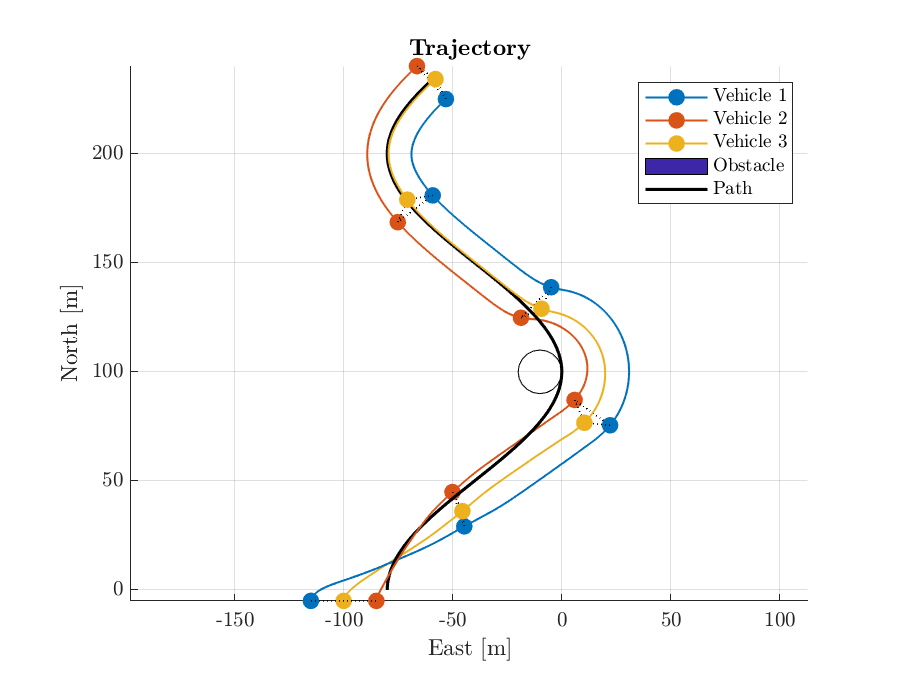
\includegraphics[width=.8\textwidth]{figures/sim-three-agent-general/plot3d-trajectory.eps}
    \vspace*{-4mm}
    \caption{The trajectory of the vehicles. The markers represent the vehicle positions every 50 seconds.}
    \label{fig:plot3d-general-mission}
    \vspace{-4mm}
\end{figure}


\begin{figure}[htbp]
    \centering
    \begin{subfigure}[t]{.9\textwidth}
    \centering
    \setlength\figurewidth{.8\linewidth}
    \setlength\figureheight{3cm}
    % This file was created by matlab2tikz.
%
%The latest updates can be retrieved from
%  http://www.mathworks.com/matlabcentral/fileexchange/22022-matlab2tikz-matlab2tikz
%where you can also make suggestions and rate matlab2tikz.
%
\definecolor{mycolor1}{rgb}{0.00000,0.44700,0.74100}%
\definecolor{mycolor2}{rgb}{0.85000,0.32500,0.09800}%
%
\begin{tikzpicture}

\begin{axis}[%
width=0.951\figurewidth,
height=\figureheight,
at={(0\figurewidth,0\figureheight)},
scale only axis,
xmin=0,
xmax=250,
xlabel style={at={(axis description cs:0.5,-0.08)}, font=\color{white!15!black}},
xlabel={Time [s]},
ymin=0,
ymax=25,
ylabel style={font=\color{white!15!black}, yshift=2mm},
ylabel={Distance [m]},
axis background/.style={fill=white},
every axis plot/.append style={line width=0.7pt},
title style={font=\bfseries, yshift=-2.75mm},
title={Smallest distances},
legend style={at={(0.97,0.02)}, anchor=south east, legend cell align=left, align=left, draw=white!15!black, legend columns=2,font=\footnotesize}
]
\addplot [color=mycolor1]
  table[]{collision_avoidance-1.tsv};
\addlegendentry{Inter-vehicle}

\addplot [color=mycolor2]
  table[]{collision_avoidance-2.tsv};
\addlegendentry{Obstacle}

\addplot[area legend, dashed, draw=black, fill=green, fill opacity=0.15, forget plot]
table[] {formation_keeping_error-10.tsv}--cycle;

\addplot [color=black, dashed]
  table[]{collision_avoidance-3.tsv};
\addlegendentry{$d_{\rm COLAV}$}


\addplot[area legend, dashed, draw=black, fill=white!50!red, fill opacity=0.25, forget plot]
table[] {collision_avoidance-4.tsv}--cycle;
\end{axis}
\end{tikzpicture}%
    \vspace*{-2mm}
    \caption{The minimum inter-vehicle and obstacle distance.}
    \label{fig:collision_avoidance}
    \end{subfigure}
    \\
    \begin{subfigure}[t]{.9\textwidth}
    \centering
    \setlength\figurewidth{.8\linewidth}
    \setlength\figureheight{3.3cm}
    % This file was created by matlab2tikz.
%
%The latest updates can be retrieved from
%  http://www.mathworks.com/matlabcentral/fileexchange/22022-matlab2tikz-matlab2tikz
%where you can also make suggestions and rate matlab2tikz.
%
\definecolor{mycolor1}{rgb}{0.00000,0.44700,0.74100}%
\definecolor{mycolor2}{rgb}{0.85000,0.32500,0.09800}%
\definecolor{mycolor3}{rgb}{0.92900,0.69400,0.12500}%
%
\begin{tikzpicture}

\begin{axis}[%
width=0.951\figurewidth,
height=\figureheight,
at={(0\figurewidth,0\figureheight)},
scale only axis,
xmin=0,
xmax=250,
xlabel style={at={(axis description cs:0.5,-0.08)}, font=\color{white!15!black}},
xlabel={Time [s]},
ymin=-25,
ymax=25,
ylabel style={font=\color{white!15!black}},
ylabel={Error [m]},
axis background/.style={fill=white},
every axis plot/.append style={line width=0.7pt},
title style={font=\bfseries, yshift=-2.75mm},
title={Formation keeping errors},
axis background/.style={fill=white},
legend style={legend cell align=left, align=left, draw=white!15!black,font=\footnotesize}
]
\addplot [color=mycolor1]
table[]{formation_keeping_error-1.tsv};
\addlegendentry{$x$-error}

\addplot [color=mycolor1, dashed, forget plot]
table[]{formation_keeping_error-2.tsv};
\addplot [color=mycolor1, dotted, forget plot]
table[]{formation_keeping_error-3.tsv};
\addplot [color=mycolor2]
table[]{formation_keeping_error-4.tsv};
\addlegendentry{$y$-error}

\addplot [color=mycolor2, dashed, forget plot]
table[]{formation_keeping_error-5.tsv};
\addplot [color=mycolor2, dotted, forget plot]
table[]{formation_keeping_error-6.tsv};
\addplot [color=mycolor3]
table[]{formation_keeping_error-7.tsv};
\addlegendentry{$z$-error}

\addplot [color=mycolor3, dashed, forget plot]
table[]{formation_keeping_error-8.tsv};
\addplot [color=mycolor3, dotted, forget plot]
table[]{formation_keeping_error-9.tsv};

\addplot[area legend, dashed, draw=black, fill=green, fill opacity=0.15, forget plot]
table[] {formation_keeping_error-10.tsv}--cycle;

\addplot[area legend, dashed, draw=black, fill=white!50!red, fill opacity=0.25, forget plot]
table[] {formation_keeping_error-11.tsv}--cycle;
\end{axis}

% \begin{axis}[%
% width=1.227\figurewidth,
% height=1.227\figureheight,
% at={(-0.16\figurewidth,-0.135\figureheight)},
% scale only axis,
% xmin=0,
% xmax=1,
% ymin=0,
% ymax=1,
% axis line style={draw=none},
% ticks=none,
% axis x line*=bottom,
% axis y line*=left
% ]
% \end{axis}
\end{tikzpicture}%
    \vspace*{-2mm}
    \caption{The formation keeping errors. }
    \label{fig:formation_keeping_error}
    \end{subfigure}
    \\
    \begin{subfigure}[t]{.9\textwidth}
    \centering
    \setlength\figurewidth{.8\linewidth}
    \setlength\figureheight{3cm}
    % This file was created by matlab2tikz.
%
%The latest updates can be retrieved from
%  http://www.mathworks.com/matlabcentral/fileexchange/22022-matlab2tikz-matlab2tikz
%where you can also make suggestions and rate matlab2tikz.
%
\definecolor{mycolor1}{rgb}{0.00000,0.44700,0.74100}%
\definecolor{mycolor2}{rgb}{0.85000,0.32500,0.09800}%
\definecolor{mycolor3}{rgb}{0.92900,0.69400,0.12500}%
%
\begin{tikzpicture}

\begin{axis}[%
width=0.951\figurewidth,
height=\figureheight,
at={(0\figurewidth,0\figureheight)},
scale only axis,
xmin=0,
xmax=250,
xlabel style={at={(axis description cs:0.5,-0.08)}, font=\color{white!15!black}},
xlabel={Time [s]},
ymin=-20,
ymax=20,
ylabel style={font=\color{white!15!black}},
ylabel={Error [m]},
every axis plot/.append style={line width=0.7pt},
every axis plot/.append style={thick},
title style={font=\bfseries, yshift=-2.75mm},
title={Path following error},
legend style={legend cell align=left, align=left, draw=white!15!black,font=\footnotesize}
]
\addplot [color=mycolor1]
  table[]{path_following_error-1.tsv};
\addlegendentry{$x$-error}

\addplot [color=mycolor2]
  table[]{path_following_error-2.tsv};
\addlegendentry{$y$-error}

\addplot [color=mycolor3]
  table[]{path_following_error-3.tsv};
\addlegendentry{$z$-error}


\addplot[area legend, dashed, draw=black, fill=green, fill opacity=0.15, forget plot]
table[] {path_following_error-4.tsv}--cycle;
\end{axis}
\end{tikzpicture}%
    \vspace*{-2mm}
    \caption{The path-following error of the barycenter.}
    \label{fig:path_following_error}
    \end{subfigure}
    \vspace*{-2mm}
    \caption{Error variables from the simulated mission. The full, dashed, and dotted lines correspond to the three different vehicles. The green and red rectangles represent when obstacle avoidance or inter-vehicle COLAV is active.}
    \label{fig:sim_results}
\end{figure}

The resulting North-East trajectory of the mission is shown in Figure~\ref{fig:plot3d-general-mission}. The vehicles avoid the obstacle with a margin and return to the desired path. The fleet deviates from the desired path right away, because the path is inside the obstacle's collision cone as illustrated in Figure~\ref{fig:collision_cone}. The avoidance maneuver is further detailed in Figure~\ref{fig:collision_avoidance}. The collision cones avoidance task is active from the beginning of the mission until the obstacle is passed. In other words, the fleet proactively changes its path early in order to avoid the obstacle. The minimum distance between the fleet and the obstacle is $10\, \mathrm{m}$ as expected when the obstacle avoidance radius $r_o$ is chosen $10 \, \mathrm{m}$ larger than the obstacle radius. The distance is at its minimum at the 100-second mark. Then, it can be seen from the third set of markers in Figure~\ref{fig:plot3d-general-mission} that the fleet path is tangent to the obstacle, which is the expected behavior of the collision cones avoidance method. Figure~\ref{fig:collision_avoidance} further shows that the inter-vehicle COLAV task activates when the distance between vehicles is below $d_{COLAV} = 10\, \mathrm{m}$. The distance slightly oscillates below the threshold. The oscillation can be expected because $k_{p,1}$ and $k_{d,1}$ are chosen so that the system is underdamped. The distance can reduce slightly below the threshold because the task does not activate before the threshold is violated. 



Figure~\ref{fig:formation_keeping_error} shows that the fleet converges to the desired formation during the obstacle avoidance maneuver. The obstacle avoidance task specifies common accelerations to all vehicles and does therefore not interfere with the formation-keeping task. Except for during the inter-vehicle collision avoidance, the convergence seems linear, which can be expected because the task velocity is saturated by $v_{2,\max}$. The formation-keeping errors asymptotically converge to zero in accordance with Theorem~\ref{theorem:formation_keeping}.

Figure~\ref{fig:path_following_error} shows that the path-following error initially increases as the fleet avoids the obstacle because the $x$- and $y$-components of $\mathbf{v}_{LOS,d}$ and $\dot{\mathbf{v}}_{LOS,d}$ are replaced with $\mathbf{v}_{OA,d}$ and $\dot{\mathbf{v}}_{OA,d}$ given by \eqref{eq:v_OA}, \eqref{eq:v_OA_dot}. As expected from Theorem~\ref{theorem:path_following}, the error converges to zero after the obstacle is passed when the LOS task is activated again. The constant ocean current is accurately compensated for by the integral action, and the path-following error remains at zero for the rest of the mission.

\begin{figure}[htbp]
    \centering
    \begin{subfigure}[t]{\textwidth}
    \centering
    \setlength\figurewidth{.8\linewidth}
    \setlength\figureheight{4cm}
    % This file was created by matlab2tikz.
%
%The latest updates can be retrieved from
%  http://www.mathworks.com/matlabcentral/fileexchange/22022-matlab2tikz-matlab2tikz
%where you can also make suggestions and rate matlab2tikz.
%
\definecolor{mycolor1}{rgb}{0.00000,0.44700,0.74100}%
\definecolor{mycolor2}{rgb}{0.85000,0.32500,0.09800}%
\definecolor{mycolor3}{rgb}{0.92900,0.69400,0.12500}%
%
\begin{tikzpicture}

\begin{axis}[%
width=0.951\figurewidth,
height=\figureheight,
at={(0\figurewidth,0\figureheight)},
scale only axis,
xmin=0,
xmax=250,
xlabel style={at={(axis description cs:0.5,-0.08)}, font=\color{white!15!black}},
xlabel={Time [s]},
ymin=-0.2,
ymax=0.3,
ylabel style={font=\color{white!15!black}},
ylabel={Angular Velocity [rad/s]},
axis background/.style={fill=white},
every axis plot/.append style={line width=0.7pt},
title style={font=\bfseries, yshift=-2.75mm},
title={Angular velocities},
legend style={legend cell align=left, align=left, draw=white!15!black, font=\footnotesize}
]
\addplot [color=mycolor1]
  table[]{angular_velocities-1.tsv};
\addlegendentry{Roll rate}

\addplot [color=mycolor1, dashed, forget plot]
  table[]{angular_velocities-2.tsv};
\addplot [color=mycolor1, dotted, forget plot]
  table[]{angular_velocities-3.tsv};
\addplot [color=mycolor2]
  table[]{angular_velocities-4.tsv};
\addlegendentry{Pitch rate}

\addplot [color=mycolor2, dashed, forget plot]
  table[]{angular_velocities-5.tsv};
\addplot [color=mycolor2, dotted, forget plot]
  table[]{angular_velocities-6.tsv};
\addplot [color=mycolor3]
  table[]{angular_velocities-7.tsv};
\addlegendentry{Yaw rate}

\addplot [color=mycolor3, dashed, forget plot]
  table[]{angular_velocities-8.tsv};
\addplot [color=mycolor3, dotted, forget plot]
  table[]{angular_velocities-9.tsv};

\addplot[area legend, dashed, draw=black, fill=green, fill opacity=0.15, forget plot]
table[] {angular_velocities-10.tsv}--cycle;
\end{axis}

% \begin{axis}[%
% width=1.227\figurewidth,
% height=1.227\figureheight,
% at={(-0.16\figurewidth,-0.135\figureheight)},
% scale only axis,
% xmin=0,
% xmax=1,
% ymin=0,
% ymax=1,
% axis line style={draw=none},
% ticks=none,
% axis x line*=bottom,
% axis y line*=left
% ]
% \end{axis}
\end{tikzpicture}%
    \vspace*{-3mm}
    \caption{The angular velocities of the vehicles. Dashed and dotted lines represent different vehicles.}
    \label{fig:angular_velocities}
    \end{subfigure}
    \begin{subfigure}[t]{\textwidth}
    \centering
    \setlength\figurewidth{.8\linewidth}
    \setlength\figureheight{4cm}
    % This file was created by matlab2tikz.
%
%The latest updates can be retrieved from
%  http://www.mathworks.com/matlabcentral/fileexchange/22022-matlab2tikz-matlab2tikz
%where you can also make suggestions and rate matlab2tikz.
%
\definecolor{mycolor1}{rgb}{0.00000,0.44700,0.74100}%
\definecolor{mycolor2}{rgb}{0.85000,0.32500,0.09800}%
\definecolor{mycolor3}{rgb}{0.92900,0.69400,0.12500}%
%
\begin{tikzpicture}

\begin{axis}[%
width=0.951\figurewidth,
height=\figureheight,
at={(0\figurewidth,0\figureheight)},
scale only axis,
xmin=0,
xmax=250,
xlabel style={at={(axis description cs:0.5,-0.08)}, font=\color{white!15!black}},
xlabel={Time [s]},
ymin=0.5,
ymax=2,
ylabel style={font=\color{white!15!black}},
ylabel={Velocity [m/s]},
axis background/.style={fill=white},
every axis plot/.append style={line width=0.7pt},
title style={font=\bfseries, yshift=-2.75mm},
title={Surge velocity},
axis background/.style={fill=white},
legend style={legend pos= south east, legend cell align=left, align=left,  draw=white!15!black, font=\footnotesize}
]
\addplot [color=mycolor1]
  table[]{surge_velocity-1.tsv};
\addlegendentry{First vehicle}
  
\addplot [color=mycolor2]
  table[]{surge_velocity-2.tsv};
\addlegendentry{Second vehicle}
\addplot [color=mycolor3]
  table[]{surge_velocity-3.tsv};
\addlegendentry{Third vehicle}
\addplot [color=black, dashed, forget plot]
  table[]{surge_velocity-4.tsv};

\addplot[area legend, dashed, draw=black, fill=green, fill opacity=0.15, forget plot]
table[] {surge_velocity-5.tsv}--cycle;
\end{axis}
\end{tikzpicture}%
    \vspace*{-3mm}
    \caption{The surge velocities of the vehicles.}
    \label{fig:surge_velocities}
    \end{subfigure}
    \caption{Angular and surge velocities for the vehicles in the first simulated mission. The green rectangle represents the time when the collision avoidance task was active.}
    \label{fig:velocities}
\end{figure}


Figure~\ref{fig:angular_velocities} shows that the angular velocities remain bounded, in accordance with Theorem~\ref{theorem:angular_velocities}. Figure~\ref{fig:surge_velocities} shows that the surge velocities of all vehicles remain between $1\, \mathrm{m/s}$ and $2\, \mathrm{m/s}$, which is expected, as the velocity should remain in the interval $U_{LOS} \pm v_{2_{\max}} = [0.75, \; 2.25]$, except for during inter-vehicle collision avoidance maneuvers. Furthermore, this range includes the expected operating surge velocity of the vehicle the simulation is modeled after.

% \begin{figure}[htb]
%     \centering
%     \begin{subfigure}[t]{.9\textwidth}
%     \centering
%     \setlength\figurewidth{.8\linewidth}
%     \setlength\figureheight{2.8cm}
%     \input{tikz_figures/nsb_mu_norm}
%     \vspace*{-2mm}
%     \caption{The norm of the virtual input $\bm{\mu}$. }
%     \label{fig:nsb_mu_norm}
%     \end{subfigure}
%     \\
%     \begin{subfigure}[t]{.9\textwidth}
%     \centering
%     \setlength\figurewidth{.8\linewidth}
%     \setlength\figureheight{2.8cm}
%     % This file was created by matlab2tikz.
%
%The latest updates can be retrieved from
%  http://www.mathworks.com/matlabcentral/fileexchange/22022-matlab2tikz-matlab2tikz
%where you can also make suggestions and rate matlab2tikz.
%
\definecolor{mycolor1}{rgb}{0.00000,0.44700,0.74100}%
\definecolor{mycolor2}{rgb}{0.85000,0.32500,0.09800}%
\definecolor{mycolor3}{rgb}{0.92900,0.69400,0.12500}%
%
\begin{tikzpicture}

\begin{axis}[%
width=0.951\figurewidth,
height=\figureheight,
at={(0\figurewidth,0\figureheight)},
scale only axis,
xmin=0,
xmax=250,
xlabel style={font=\color{white!15!black}},
xlabel={Time [s]},
ymin=-15,
ymax=15,
ylabel style={font=\color{white!15!black}},
ylabel={$T_u$ [N]},
axis background/.style={fill=white},
title style={font=\bfseries, yshift=-2mm},
title={\textbf{Surge thrust}},
legend style={legend cell align=left, align=left, draw=white!15!black, font=\footnotesize}
]
\addplot [color=mycolor1]
  table[]{nsb_surge_thrust-1.tsv};
\addlegendentry{Vehicle 1}

\addplot [color=mycolor2]
  table[]{nsb_surge_thrust-2.tsv};
\addlegendentry{Vehicle 2}

\addplot [color=mycolor3]
  table[]{nsb_surge_thrust-3.tsv};
\addlegendentry{Vehicle 3}


\addplot[area legend, dashed, draw=black, fill=white!50!red, fill opacity=0.25, forget plot]
table[] {nsb_surge_thrust-4.tsv}--cycle;
\end{axis}

\begin{axis}[%
width=1.227\figurewidth,
height=1.227\figureheight,
at={(-0.16\figurewidth,-0.135\figureheight)},
scale only axis,
xmin=0,
xmax=1,
ymin=0,
ymax=1,
axis line style={draw=none},
ticks=none,
axis x line*=bottom,
axis y line*=left
]
\end{axis}
\end{tikzpicture}%
%     \vspace*{-2mm}
%     \caption{The commanded surge thrust.}
%     \label{fig:nsb_surge_thrust}
%     \end{subfigure}
%     \vspace*{-2mm}
%     \caption{Control inputs from the simulation of the second-order NSB algorithm with collision cones obstacle avoidance.}
%     \label{fig:nsb_control_inputs}
% \end{figure}

% As discussed in Chapter~\ref{cha:consensus_algorithms} an algorithm with theoretical guarantees for stability and collision avoidance may still be unsuited for practical implementation if it requires unphysical actuation. Figure~\ref{fig:nsb_control_inputs} shows that the commanded virtual control inputs $\bm{\mu}$ and surge thrust $T_u$ are within reasonable limits for the second-order NSB algorithm.


\subsection{Individual obstacle avoidance}\label{sec:individual_obstacle}
In this section, we examine a simulation study of the \gls{nsb} formation path-following problem with the obstacle avoidance method from Section~\ref{sec:individual_colav} adapted from \cite{arrichiello_formation_2006}. A key difference from the collision cones method simulated in the previous section is that this method enables the fleet to break formation in order to avoid collisions. Furthermore, this method enables the vehicles to conduct avoidance maneuvers in all three dimensions and not only in the $xy$ plane.\enlargethispage*{\baselineskip}

\begin{figure}[htb]
    \centering
    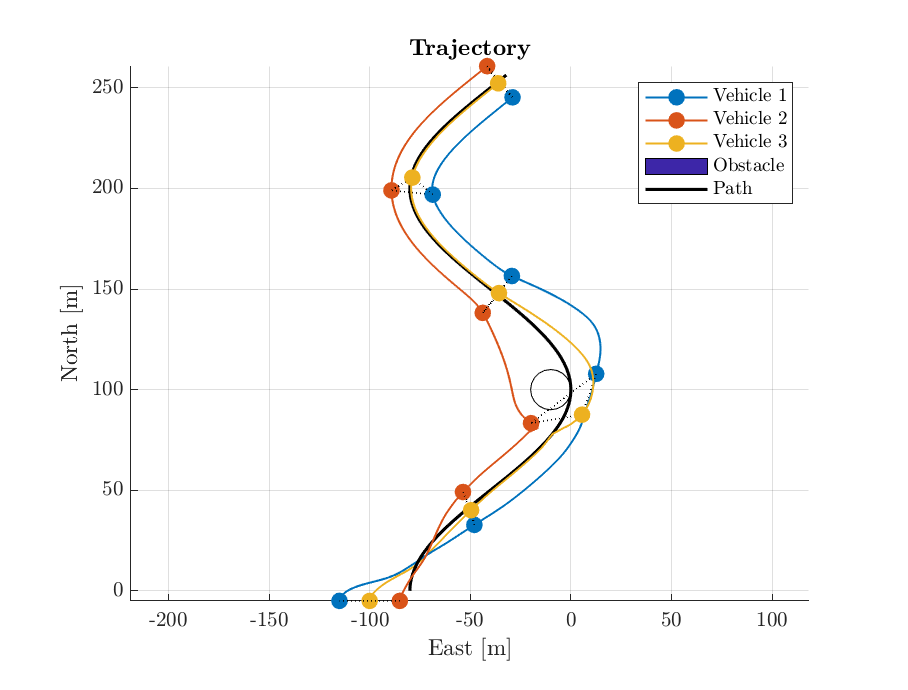
\includegraphics[width=.8\textwidth]{figures/plot3d_IC.eps}
    \vspace*{-4mm}
    \caption{The trajectory of the vehicles. The markers represent the vehicle positions every 50 seconds.}
    \label{fig:plot3d-IC}
    \vspace{-2mm}
\end{figure}

The simulation setup is similar to the previous section, with the same desired path, external obstacle, constant ocean current, and initial states. Furthermore, all controller gains and parameters are also the same, given by Table~\ref{tab:simulation_parameters1}.

The resulting trajectory in the NED coordinate frame is shown in Figure~\ref{fig:plot3d-IC}. The fleet splits up the formation to pass the obstacle and converges back to the formation after the obstacle is passed. Compared to the collision cones avoidance method, the fleet deviates late from the path in order to avoid the obstacle, which is further shown in Figure~\ref{fig:collision_avoidance_IC}, where the green rectangle represents when the external collision avoidance task is active. As also seen in Figure~\ref{fig:collision_avoidance_IC}, the inter-vehicle collision avoidance still works well, despite now being defined as individual tasks for each vehicle, which is expected because the formulation with individual tasks should be equivalent to the joint formulation, as long as only two vehicles are within the collision threshold of each other.

Figure~\ref{fig:path_following_error_IC} shows that the fleet converges earlier to the correct path and deviates minimally from it during the avoidance maneuver. The limited deviation is possible because the path error is defined in terms of the barycenter, and as long as some vehicles of the fleet are on each side of the obstacle, it is possible for the barycenter to remain on the path. Instead, the formation-keeping error increases during the avoidance maneuver, as seen in Figure~\ref{fig:formation_keeping_error_IC}. With the collision cones avoidance method from the previous section, the formation was kept during obstacle avoidance. 

\begin{figure}[htbp]
    \centering
    \begin{subfigure}[t]{.9\textwidth}
    \centering
    \setlength\figurewidth{.8\linewidth}
    \setlength\figureheight{3cm}
    \input{tikz_figures/individual_colav_collision_avoidance}
    \vspace*{-2mm}
    \caption{The minimum inter-vehicle and obstacle distance.}
    \label{fig:collision_avoidance_IC}
    \end{subfigure}
    \\
    \begin{subfigure}[t]{.9\textwidth}
    \centering
    \setlength\figurewidth{.8\linewidth}
    \setlength\figureheight{3.3cm}
    \input{tikz_figures/individual_colav_formation_keeping_error}
    \vspace*{-2mm}
    \caption{The formation keeping errors. }
    \label{fig:formation_keeping_error_IC}
    \end{subfigure}
    \\
    \begin{subfigure}[t]{.9\textwidth}
    \centering
    \setlength\figurewidth{.8\linewidth}
    \setlength\figureheight{3cm}
    \input{tikz_figures/individual_colav_path_following_error}
    \vspace*{-2mm}
    \caption{The path-following error of the barycenter.}
    \label{fig:path_following_error_IC}
    \end{subfigure}
    \vspace*{-2mm}
    \caption{Error variables from the second simulated mission. The full, dashed, and dotted lines correspond to the three different vehicles. The green and red rectangles represent when obstacle avoidance or inter-vehicle COLAV is active.}
    \label{fig:sim_results_IC}
\end{figure}

\begin{figure}[htbp]
    \centering
    \begin{subfigure}[t]{\textwidth}
    \centering
    \setlength\figurewidth{.8\linewidth}
    \setlength\figureheight{4cm}
    \input{tikz_figures/individual_colav_angular_velocities}
    % \vspace*{-3mm}
    \caption{The angular velocities of the vehicles. Dashed and dotted lines represent different vehicles.}
    \label{fig:angular_velocities_IC}
    \end{subfigure}
    \begin{subfigure}[t]{\textwidth}
    \centering
    \setlength\figurewidth{.8\linewidth}
    \setlength\figureheight{4cm}
    \input{tikz_figures/individual_colav_surge_velocity}
    % \vspace*{-3mm}
    \caption{The surge velocities of the vehicles.}
    \label{fig:surge_velocities_IC}
    \end{subfigure}
    \caption{Angular and surge velocities for the vehicles in the second simulated mission. The green rectangle represents the time when the collision avoidance task was active.}
    \label{fig:velocities_IC}
\end{figure}

Figure~\ref{fig:surge_velocities_IC} shows that the surge velocities of the vehicles rise above $3\, \mathrm{m/s}$ and sink below $0.5\, \mathrm{m/s}$. Velocities above $3\, \mathrm{m/s}$ are unexpected, as it is above the maximum operating velocity of the physical vehicles that the simulation models. There are two possible explanations for such a high velocity. First, the controller might command generalized forces that are larger than the limits of the physical systems actuators. Actuator saturation was not modeled, and such forces would be applied directly to the plant in our simulator. In a real system with actuation limits, the control action going into saturation might impose a stability problem. A second explanation for the large surge velocities is that the simulation does not model non-linear damping. In a more realistic simulator, the non-linear damping would become significant when the velocities increase above the nominal operating range. It is also problematic that the velocity of a vehicle sinks below $0.5\, \mathrm{m/s}$. Then, a real, physical vehicle would lose controllability because water does not flow sufficiently fast past the fins.

\begin{figure}[htb]
    \centering
    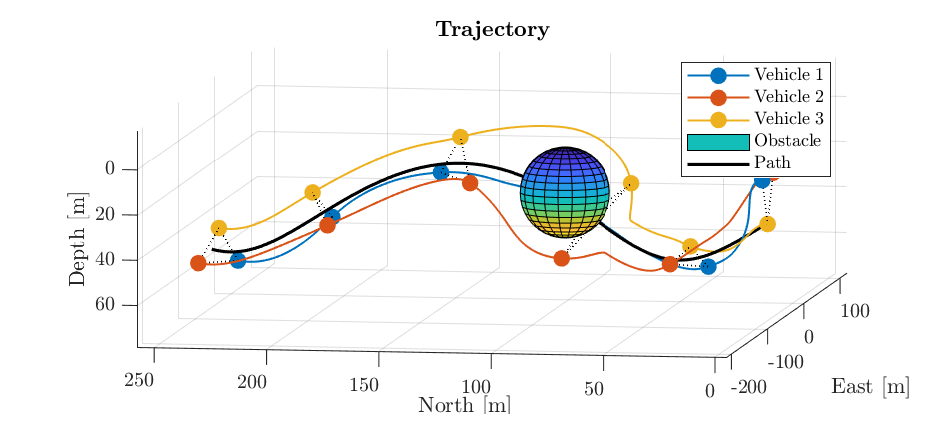
\includegraphics[width=.9\textwidth]{figures/plot3d_sphere.eps}
    \vspace{-3mm}
    \caption{Illustration of obstacle avoidance in all three dimensions. The obstacle is chosen as a sphere.}
    \label{fig:sphere_avoidance}
    \vspace{-4mm}
\end{figure}

Another feature that distinguishes this obstacle avoidance method from the collision cones method is that it enables obstacle avoidance in all three dimensions. In the collision cones method, the avoidance maneuver was limited to the $xy$-plane. As demonstrated in Figure~\ref{fig:sphere_avoidance}, the obstacle avoidance method as described in Section~\ref{sec:individual_colav} enables each individual vehicle to independently avoid the obstacle in all dimensions. The spherical obstacle in this experiment was chosen larger than the cylindrical obstacle in the previous experiments for illustrative purposes.

\subsection{Formation error as damped harmonic motion}\label{sec:harmonic_motion}
Part of the motivation for developing the second-order \gls{nsb} controller is that there are no hidden dynamics abstracted away in the low-level control layer. Consequently, the collision-avoidance and formation-keeping error systems are expected to behave exactly as second-order systems defined by the gain matrices. In turn, the gain matrices can be chosen by specifying natural frequencies and damping ratios as described in Section~\ref{sec:nsb_second_order}. In this section, we will observe the transient of the formation-keeping error under different controller gains. Although we demonstrate the concept with the formation-keeping error, the same behavior is expected for the collision-avoidance task as well.

We design a simple simulation experiment in which everything except for the formation-keeping task is simplified as much as possible. The fleet is made to follow a straight line in the north direction. It is initialized with the barycenter on the path, and there is no external obstacle or ocean current. The desired formation is given by \eqref{eq:desired_formation_sim} as in the previous simulation experiments, and the initial relative positions are given by $\bm{\sigma}_{2,i} = 2\mathbf{p}_{f,i}^f$. All controller gains and parameters except for $k_{p,2}$ and $k_{d,2}$ are given by Table~\ref{tab:simulation_parameters1}. We simulate three different choices of formation-keeping controller gains given by Table~\ref{tab:controller-params}. The natural frequency is kept fixed at $\omega_{n,2} = 0.5$ which is low enough so that the effects of the saturation in the controller are minimal, and the damping ratio is chosen so that the system is underdamped, critically damped, and overdamped for the respective three experiments. The total simulation time is $50\, \mathrm{s}$.

\begin{table}[h]
\centering
\caption{Controller parameters for the three experiments.}
\label{tab:controller-params}
\begin{tabular}{lccc}
\hline
Parameter & Experiment 1 & Experiment 2 & Experiment 3 \\ \hline
$\omega_{n,2}$ & 0.5 & 0.5 & 0.5 \\
$\xi_2$ & 0.3 & 1 & 2 \\
$k_{p,2}$ & 0.25 & 0.25 & 0.25 \\
$k_{d,2}$ & 0.3 & 1 & 2 \\ \hline
\end{tabular}
\end{table}

\begin{figure}[htbp]
    \centering
    \begin{subfigure}[t]{.9\textwidth}
    \centering
    \setlength\figurewidth{.8\linewidth}
    \setlength\figureheight{3.8cm}
    \input{tikz_figures/underdamped_3d_plot}
    \vspace*{-4mm}
    \caption{The underdamped system.}
    \label{fig:underdamped_3d}
    \end{subfigure}
    \vspace*{-.9mm}
    \\
    \begin{subfigure}[t]{.9\textwidth}
    \centering
    \setlength\figurewidth{.8\linewidth}
    \setlength\figureheight{3.8cm}
    \input{tikz_figures/critically_damped_3d_plot}
    \vspace*{-4mm}
    \caption{The critically damped system. }
    \label{fig:critically_damped_3d}
    \end{subfigure}
    \vspace*{-.9mm}
    \\
    \begin{subfigure}[t]{.9\textwidth}
    \centering
    \setlength\figurewidth{.8\linewidth}
    \setlength\figureheight{3.8cm}
    % This file was created by matlab2tikz.
%
%The latest updates can be retrieved from
%  http://www.mathworks.com/matlabcentral/fileexchange/22022-matlab2tikz-matlab2tikz
%where you can also make suggestions and rate matlab2tikz.
%
\definecolor{mycolor1}{rgb}{0.00000,0.44700,0.74100}%
\definecolor{mycolor2}{rgb}{0.85000,0.32500,0.09800}%
\definecolor{mycolor3}{rgb}{0.92900,0.69400,0.12500}%
%
\begin{tikzpicture}

\begin{axis}[%
unit vector ratio*=1 1 1,
width=0.951\figurewidth,
height=\figureheight,
at={(0\figurewidth,0\figureheight)},
scale only axis,
xmin=-50.7158619100192,
xmax=50.7158619100192,
xlabel style={at={(axis description cs:0.5,-0.05)}, font=\color{white!15!black}},
xlabel={East [m]},
ymin=-5,
ymax=75.0001821741917,
ylabel style={font=\color{white!15!black}},
ylabel={North [m]},
axis background/.style={fill=white},
title style={font=\bfseries, yshift=-3mm},
title={\textbf{Trajectory}},
axis x line*=bottom,
axis y line*=left,
xmajorgrids,
ymajorgrids,
legend style={legend cell align=left, align=left, draw=white!15!black, font=\footnotesize}
]

\addplot [color=black, line width=1.5pt]
  table[]{overdamped_3d_plot-4.tsv};
\addlegendentry{Path}


\addplot [color=mycolor1, line width=1.0pt, mark size=3.5pt, mark=*, mark options={solid, fill=mycolor1, mycolor1}, mark repeat=50]
  table[]{overdamped_3d_plot-1.tsv};
\addlegendentry{Veh. 1}

\addplot [color=mycolor2, line width=1.0pt, mark size=3.5pt, mark=*, mark options={solid, fill=mycolor2, mycolor2}, mark repeat=50]
  table[]{overdamped_3d_plot-2.tsv};
\addlegendentry{Veh. 2}

\addplot [color=mycolor3, line width=1.0pt, mark size=3.5pt, mark=*, mark options={solid, fill=mycolor3, mycolor3}, mark repeat=50]
  table[]{overdamped_3d_plot-3.tsv};
\addlegendentry{Veh. 3}



\addplot [color=black, dotted, line width=0.8pt, forget plot]
  table[]{overdamped_3d_plot-5.tsv};
\addplot [color=black, dotted, line width=0.8pt, forget plot]
  table[]{overdamped_3d_plot-6.tsv};
\addplot [color=black, dotted, line width=0.8pt, forget plot]
  table[]{overdamped_3d_plot-7.tsv};
\addplot [color=black, dotted, line width=0.8pt, forget plot]
  table[]{overdamped_3d_plot-8.tsv};
\addplot [color=black, dotted, line width=0.8pt, forget plot]
  table[]{overdamped_3d_plot-9.tsv};
\addplot [color=black, dotted, line width=0.8pt, forget plot]
  table[]{overdamped_3d_plot-10.tsv};
\addplot [color=black, dotted, line width=0.8pt, forget plot]
  table[]{overdamped_3d_plot-11.tsv};
\addplot [color=black, dotted, line width=0.8pt, forget plot]
  table[]{overdamped_3d_plot-12.tsv};
\addplot [color=black, dotted, line width=0.8pt, forget plot]
  table[]{overdamped_3d_plot-13.tsv};
\addplot [color=black, dotted, line width=0.8pt, forget plot]
  table[]{overdamped_3d_plot-14.tsv};
\end{axis}
\end{tikzpicture}%
    \vspace*{-4mm}
    \caption{The overdamped system.}
    \label{fig:overdamped_3d}
    \end{subfigure}
    \vspace*{-3.5mm}
    \caption{The north-east trajectories of the vehicles with different formation-keeping controller gains.}
    \label{fig:formation_3d_dampings}
\end{figure}


\begin{figure}[htbp]
    \centering
    \begin{subfigure}[t]{.9\textwidth}
    \centering
    \setlength\figurewidth{.8\linewidth}
    \setlength\figureheight{3cm}
    % This file was created by matlab2tikz.
%
%The latest updates can be retrieved from
%  http://www.mathworks.com/matlabcentral/fileexchange/22022-matlab2tikz-matlab2tikz
%where you can also make suggestions and rate matlab2tikz.
%
\definecolor{mycolor1}{rgb}{0.00000,0.44700,0.74100}%
\definecolor{mycolor2}{rgb}{0.85000,0.32500,0.09800}%
\definecolor{mycolor3}{rgb}{0.92900,0.69400,0.12500}%
%
\begin{tikzpicture}

\begin{axis}[%
width=0.951\figurewidth,
height=\figureheight,
at={(0\figurewidth,0\figureheight)},
scale only axis,
xmin=0,
xmax=50,
xlabel style={at={(axis description cs:0.5,-0.08)}, font=\color{white!15!black}},
xlabel={Time [s]},
ymin=-10,
ymax=10,
ylabel style={font=\color{white!15!black}},
ylabel={Error [m]},
axis background/.style={fill=white},
every axis plot/.append style={line width=0.7pt},
title style={font=\bfseries, yshift=-2mm},
title={Formation keeping error},
axis x line*=bottom,
axis y line*=left,
legend style={legend cell align=left, align=left, draw=white!15!black}
]
\addplot [color=mycolor1]
  table[]{underdamped_formation_error-1.tsv};
\addlegendentry{$x$-error}

\addplot [color=mycolor1, dashed, forget plot]
  table[]{underdamped_formation_error-2.tsv};
\addplot [color=mycolor1, dotted, forget plot]
  table[]{underdamped_formation_error-3.tsv};
\addplot [color=mycolor2]
  table[]{underdamped_formation_error-4.tsv};
\addlegendentry{$y$-error}

\addplot [color=mycolor2, dashed, forget plot]
  table[]{underdamped_formation_error-5.tsv};
\addplot [color=mycolor2, dotted, forget plot]
  table[]{underdamped_formation_error-6.tsv};
\addplot [color=mycolor3]
  table[]{underdamped_formation_error-7.tsv};
\addlegendentry{$z$-error}

\addplot [color=mycolor3, dashed, forget plot]
  table[]{underdamped_formation_error-8.tsv};
\addplot [color=mycolor3, dotted, forget plot]
  table[]{underdamped_formation_error-9.tsv};
\end{axis}
\end{tikzpicture}%
    \vspace*{-2mm}
    \caption{The underdamped system.}
    \label{fig:underdamped_formation}
    \end{subfigure}
    \\
    \begin{subfigure}[t]{.9\textwidth}
    \centering
    \setlength\figurewidth{.8\linewidth}
    \setlength\figureheight{3cm}
    \input{tikz_figures/critically_damped_formation_error}
    \vspace*{-2mm}
    \caption{The critically damped system. }
    \label{fig:critically_damped_formation}
    \end{subfigure}
    \\
    \begin{subfigure}[t]{.9\textwidth}
    \centering
    \setlength\figurewidth{.8\linewidth}
    \setlength\figureheight{3cm}
    \input{tikz_figures/overdamped_formation_error}
    \vspace*{-2mm}
    \caption{The overdamped system.}
    \label{fig:overdamped_formation}
    \end{subfigure}
    \vspace*{-2mm}
    \caption{The formation-keeping errors for the vehicles with different formation-keeping controller gains. The full, dashed, and dotted lines illustrate the different vehicles.}
    \label{fig:formation_dampings_errors}
\end{figure}

Figure~\ref{fig:formation_3d_dampings} shows the north-east trajectory for the vehicles with different damping ratios. The corresponding formation-keeping errors are shown in Figure~\ref{fig:formation_dampings_errors}. As expected, the formation-keeping error in the underdamped system exhibits an oscillatory motion. The error in the critically damped system converges quickly to the origin without oscillations, and the overdamped system converges more slowly. Despite the saturation term in the formation-keeping acceleration \eqref{eq:saturated_formation_keeping}, the task errors converge as can be expected from the theory of damped harmonic motion.

\vspace{-3mm}
\section{Distributed NSB algorithm simulation results}\label{sec:distributed_simulations}
This section presents three simulation experiments with the distributed \gls{nsb} method from Chapter~\ref{cha:distributed_NSB}. The method is first demonstrated on a general mission featuring collision avoidance, formation keeping, and path following in Section~\ref{sec:simulation_distributed_nsb}. Then, the method is compared to two existing methods from the literature in Sections~\ref{sec:comparison_distributed_NSB} and \ref{sec:comparison_restrepo}, and the alternative distributed implementation in Section~\ref{sec:sim_alternative}. The method is configured with the sliding-mode path-following acceleration given by \eqref{eq:sliding_mode_path_following}.


\subsection{General five-agent mission}\label{sec:simulation_distributed_nsb}
This section presents a simulation experiment of the distributed \gls{nsb} control law presented in Chapter~\ref{cha:distributed_NSB}. The experiment involves a fleet of five agents with a communication graph given by Figure~\ref{fig:communication_graph}. All controller gains and parameters are unchanged from previous experiments and given by Table~\ref{tab:simulation_parameters1}.
\begin{figure}[h]
    \centering
    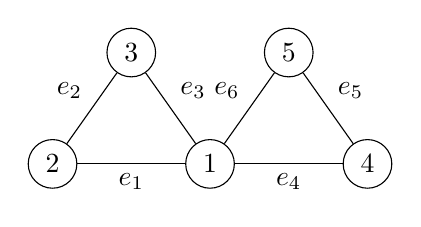
\begin{tikzpicture}
  % Nodes
  \node[circle, draw, minimum size=6mm] (1) at (0,0) {1};
  \node[circle, draw, minimum size=6mm] (2) at (-2,0) {2};
  \node[circle, draw, minimum size=6mm] (3) at (-1,{sqrt(2)}) {3};
  \node[circle, draw, minimum size=6mm] (4) at (2,0) {4};
  \node[circle, draw, minimum size=6mm] (5) at (1,{sqrt(2)}) {5};
  
  % Edges
  \foreach \x/\y/\name in {1/2/$e_1$, 2/3/$e_2$, 3/1/$e_3$, 4/1/$e_4$, 5/4/$e_5$, 1/5/$e_6$}
    \draw (\x) -- (\y) node[midway, auto] {\name};
\end{tikzpicture}
\vspace*{-4mm}
    \caption{The communication graph of the fleet.}
    \label{fig:communication_graph}
    \vspace*{-4mm}
\end{figure}


The barycenter relative vectors give the desired formation:
\begin{equation}
    \begin{split}
    \mathbf{p}_{f,1:5}^f = \begin{bmatrix}
        0 & 8 & 8 & -8 & -8\\ 0 & -8 & 8 & 8 & -8 \\ 8 & -2& -2& -2& -2
    \end{bmatrix}.
    % ,\; \mathbf{p}_{f,2}^f = &\begin{bmatrix}
    %     8 \\ -8 \\ -2
    % \end{bmatrix},\; \mathbf{p}_{f,3}^f = \begin{bmatrix}
    %     8 \\ 8 \\ -2
    % \end{bmatrix},\; \\
    % \mathbf{p}_{f,4}^f = \begin{bmatrix}
    %     -8 \\ 8 \\ -2
    % \end{bmatrix}&,\; \mathbf{p}_{f,5}^f = \begin{bmatrix}
    %     -8 \\ -8 \\ -2
    % \end{bmatrix}.
    \end{split}
\end{equation}
The desired formation-relative positions of the agents 2-5 make up a square in the $xy$-plane. The fleet is initialized so that each of the four agents starts at opposite corners of the square. The initial positions are chosen slightly closer than the desired formation so that the inter-vehicle collision avoidance task activates:
\begin{equation}
    \begin{split}
    \mathbf{p}_{1:5}(0) = \begin{bmatrix}
        0 &-5& -5& 5& 5\\ 0 & 5 & -5 & -5 & 5\\ 5 & -1.25& -1.25& -1.25& -1.25
    \end{bmatrix}.
    % ,\; \mathbf{p}_{2}(0) = &\begin{bmatrix}
    %     -5 \\ 5 \\ -1.25
    % \end{bmatrix},\; \mathbf{p}_{3}(0) = \begin{bmatrix}
    %     -5 \\ -5 \\ -1.25
    % \end{bmatrix},\; \\
    % \mathbf{p}_{4}(0) = \begin{bmatrix}
    %     5 \\ -5 \\ -1.25
    % \end{bmatrix}&,\; \mathbf{p}_{5}(0) = \begin{bmatrix}
    %     5 \\ 5 \\ -1.25
    % \end{bmatrix}.
    \end{split}
\end{equation}

The fleet avoids the obstacle and converges to the desired path as seen by Figure~\ref{fig:distributed_path_plot}. Figure~\ref{fig:distributed_sim_results} shows more clearly that the formation-keeping and path-following errors converge to and remain at zero. Figure~\ref{fig:distributed_collision_avoidance} shows that the collision avoidance task works similarly to the centralized algorithm, with only small violations of the collision-avoidance threshold. 
\begin{figure}[hb]
    \centering
    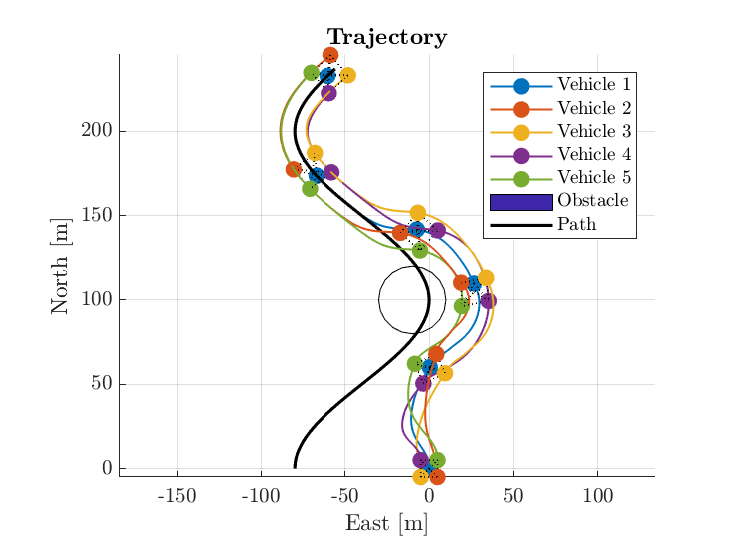
\includegraphics[width=.8\textwidth]{figures/distributed_path_plot.eps}
    \vspace{-4mm}
    \caption{The trajectory of the fleet in the North-East frame.}
    \label{fig:distributed_path_plot}
    \vspace{-4mm}
\end{figure}

\begin{figure}[htbp]
    \centering
    \begin{subfigure}[t]{.9\textwidth}
    \centering
    \setlength\figurewidth{.8\linewidth}
    \setlength\figureheight{3cm}
    % This file was created by matlab2tikz.
%
%The latest updates can be retrieved from
%  http://www.mathworks.com/matlabcentral/fileexchange/22022-matlab2tikz-matlab2tikz
%where you can also make suggestions and rate matlab2tikz.
%
\definecolor{mycolor1}{rgb}{0.00000,0.44700,0.74100}%
\definecolor{mycolor2}{rgb}{0.85000,0.32500,0.09800}%
%
\begin{tikzpicture}

\begin{axis}[%
width=0.951\figurewidth,
height=\figureheight,
at={(0\figurewidth,0\figureheight)},
scale only axis,
xmin=0,
xmax=250,
xlabel style={font=\color{white!15!black}},
xlabel={Time [s]},
ymin=0,
ymax=20,
ylabel style={font=\color{white!15!black}, yshift=2mm},
ylabel={Distance [m]},
axis background/.style={fill=white},
every axis plot/.append style={line width=0.7pt},
title style={font=\bfseries, yshift=-2.75mm},
title={Smallest distances},
legend style={at={(0.97,0.02)}, anchor=south east, legend cell align=left, align=left, draw=white!15!black, legend columns=2,font=\footnotesize}
]
\addplot [color=mycolor1]
  table[]{distributed_colav-1.tsv};
\addlegendentry{Inter-vehicle distance}

\addplot [color=mycolor2]
  table[]{distributed_colav-2.tsv};
\addlegendentry{Distance to obstacle}

\addplot [color=black, dashed]
  table[]{distributed_colav-3.tsv};
\addlegendentry{$d_{\rm COLAV}$}


\addplot[area legend, dashed, draw=black, fill=white!50!red, fill opacity=0.25, forget plot]
table[] {distributed_colav-4.tsv}--cycle;

\addplot[area legend, dashed, draw=black, fill=green, fill opacity=0.15, forget plot]
table[] {distributed_colav-5.tsv}--cycle;
\end{axis}

\begin{axis}[%
width=1.227\figurewidth,
height=1.227\figureheight,
at={(-0.16\figurewidth,-0.135\figureheight)},
scale only axis,
xmin=0,
xmax=1,
ymin=0,
ymax=1,
axis line style={draw=none},
ticks=none,
axis x line*=bottom,
axis y line*=left
]
\end{axis}
\end{tikzpicture}%
    \vspace*{-2mm}
    \caption{The minimum inter-vehicle and obstacle distance.}
    \label{fig:distributed_collision_avoidance}
    \end{subfigure}
    \\
    \begin{subfigure}[t]{.9\textwidth}
    \centering
    \setlength\figurewidth{.8\linewidth}
    \setlength\figureheight{3cm}
    % This file was created by matlab2tikz.
%
%The latest updates can be retrieved from
%  http://www.mathworks.com/matlabcentral/fileexchange/22022-matlab2tikz-matlab2tikz
%where you can also make suggestions and rate matlab2tikz.
%
\definecolor{mycolor1}{rgb}{0.00000,0.44700,0.74100}%
\definecolor{mycolor2}{rgb}{0.85000,0.32500,0.09800}%
\definecolor{mycolor3}{rgb}{0.92900,0.69400,0.12500}%
%
\begin{tikzpicture}

\begin{axis}[%
width=0.951\figurewidth,
height=\figureheight,
at={(0\figurewidth,0\figureheight)},
scale only axis,
xmin=0,
xmax=250,
xlabel style={font=\color{white!15!black}},
xlabel={Time [s]},
ymin=-15,
ymax=15,
ylabel style={font=\color{white!15!black}},
ylabel={Error [m]},
axis background/.style={fill=white},
title style={font=\bfseries, yshift=-2.75mm},
title={Formation keeping errors},
axis background/.style={fill=white},
every axis plot/.append style={line width=0.7pt},
legend style={legend cell align=left, align=left, draw=white!15!black,font=\footnotesize}
]
\addplot [color=mycolor1]
  table[]{distributed_formation_keeping-1.tsv};
  \addlegendentry{$x$-error}
\addplot [color=mycolor1, dashed, forget plot]
  table[]{distributed_formation_keeping-2.tsv};
\addplot [color=mycolor1, dotted, forget plot]
  table[]{distributed_formation_keeping-3.tsv};
\addplot [color=mycolor1, dashdotted, forget plot]
  table[]{distributed_formation_keeping-4.tsv};
\addplot [color=mycolor1, forget plot]
  table[]{distributed_formation_keeping-5.tsv};
\addplot [color=mycolor2]
  table[]{distributed_formation_keeping-6.tsv};
\addlegendentry{$y$-error}
\addplot [color=mycolor2, dashed, forget plot]
  table[]{distributed_formation_keeping-7.tsv};
\addplot [color=mycolor2, dotted, forget plot]
  table[]{distributed_formation_keeping-8.tsv};
\addplot [color=mycolor2, dashdotted, forget plot]
  table[]{distributed_formation_keeping-9.tsv};
\addplot [color=mycolor2, forget plot]
  table[]{distributed_formation_keeping-10.tsv};
\addplot [color=mycolor3]
  table[]{distributed_formation_keeping-11.tsv};
  \addlegendentry{$z$-error}
\addplot [color=mycolor3, dashed, forget plot]
  table[]{distributed_formation_keeping-12.tsv};
\addplot [color=mycolor3, dotted, forget plot]
  table[]{distributed_formation_keeping-13.tsv};
\addplot [color=mycolor3, dashdotted, forget plot]
  table[]{distributed_formation_keeping-14.tsv};
\addplot [color=mycolor3, forget plot]
  table[]{distributed_formation_keeping-15.tsv};

\addplot[area legend, dashed, draw=black, fill=green, fill opacity=0.15, forget plot]
table[] {distributed_formation_keeping-16.tsv}--cycle;

\addplot[area legend, dashed, draw=black, fill=white!50!red, fill opacity=0.25, forget plot]
table[] {distributed_formation_keeping-17.tsv}--cycle;
\end{axis}

\begin{axis}[%
width=1.227\figurewidth,
height=1.227\figureheight,
at={(-0.16\figurewidth,-0.135\figureheight)},
scale only axis,
xmin=0,
xmax=1,
ymin=0,
ymax=1,
axis line style={draw=none},
ticks=none,
axis x line*=bottom,
axis y line*=left
]
\end{axis}
\end{tikzpicture}%
    \vspace*{-2mm}
    \caption{The formation keeping errors. }
    \label{fig:distributed_formation_keeping_error}
    \end{subfigure}
    \\
    \begin{subfigure}[t]{.9\textwidth}
    \centering
    \setlength\figurewidth{.8\linewidth}
    \setlength\figureheight{3cm}
    \input{tikz_figures/distributed_path_following}
    \vspace*{-2mm}
    \caption{The path-following error of the barycenter.}
    \label{fig:distributed_path_following_error}
    \end{subfigure}
    \vspace*{-2mm}
    \caption{Error variables from the simulated distributed mission. The different line styles correspond to the five different vehicles. The green and red rectangles represent when obstacle avoidance or inter-vehicle COLAV is active.}
    \label{fig:distributed_sim_results}
\end{figure}

\subsection{Comparison study with the first-order NSB method}\label{sec:comparison_distributed_NSB}
In this section, we compare our distributed \gls{nsb} method with the first-order \gls{nsb} method from \cite{matous_formation_2023}. The Simulink model for the first-order method was provided by Josef Matou\v{s}. The first-order method is implemented in a  distributed manner as described in Section~\ref{sec:alternative_distributed}. 

We simulate the two methods on the four-vehicle simulation experiment detailed in \cite{matous_formation_2023}. We choose the experiment without obstacles because the two methods implement obstacle avoidance differently. Furthermore, the inter-vehicle collision avoidance threshold is chosen small enough for the task to not activate because the provided implementation of the first-order \gls{nsb} does not include that task. The barycenter should follow an elliptic path given by
\begin{equation}
    \mathbf{p}_p(\xi) = [a \cos{\xi},\, b \sin{\xi},\, c\sin{\xi}^2]\T,
\end{equation}
where $a = 60\, \mathrm{m}$, $b = 40\, \mathrm{m}$, $c = 10\, \mathrm{m}$. The shape of the desired formation is given by 
\begin{equation}
    \mathbf{p}_{f,1:4}^f = \begin{bmatrix}
      10& -10&  0&   0\\
      0&   0& 10& -10\\
      0&  -4&  4&   0
    \end{bmatrix},
\end{equation}
and the communication graph is given by Figure~\ref{fig:communication_graph_comparison}.
\begin{figure}[hb]
    \centering
     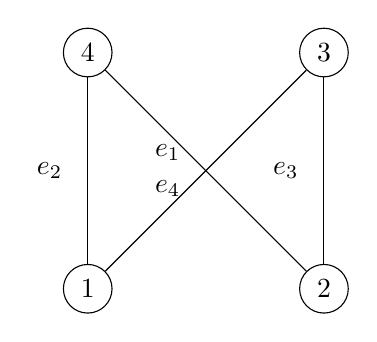
\begin{tikzpicture}
  % Nodes
  \node[circle, draw, minimum size=6mm] (1) at (0,0) {1};
  \node[circle, draw, minimum size=6mm] (2) at (3,0) {2};
  \node[circle, draw, minimum size=6mm] (3) at (3,3) {3};
  \node[circle, draw, minimum size=6mm] (4) at (0,3) {4};
  
  % Edges
  \foreach \x/\y/\name in {1/3/$e_1$, 1/4/$e_2$, 2/3/$e_3$, 2/4/$e_4$}
    \draw (\x) -- (\y) node[midway,auto, xshift=-2mm] {\name};
\end{tikzpicture}
    \caption{Communication graph for the comparison experiment.}
    \label{fig:communication_graph_comparison}
\end{figure}

\begin{figure}[ht]
    \centering
    \setlength\figurewidth{.7\textwidth}
    \setlength\figureheight{0.5\textwidth}
    % This file was created by matlab2tikz.
%
%The latest updates can be retrieved from
%  http://www.mathworks.com/matlabcentral/fileexchange/22022-matlab2tikz-matlab2tikz
%where you can also make suggestions and rate matlab2tikz.
%
\definecolor{mycolor1}{rgb}{0.00000,0.44700,0.74100}%
\definecolor{mycolor2}{rgb}{0.85000,0.32500,0.09800}%
\definecolor{mycolor3}{rgb}{0.92900,0.69400,0.12500}%
\definecolor{mycolor4}{rgb}{0.49400,0.18400,0.55600}%
%
\begin{tikzpicture}

\begin{axis}[%
% unit vector ratio*=1 1 1,
width=\figurewidth,
height=0.794\figureheight,
at={(0\figurewidth,0\figureheight)},
scale only axis,
plot box ratio=6.842 5.397 1,
xmin=-95.0778035133361,
xmax=95.1001524564096,
tick align=outside,
xlabel style={font=\color{white!15!black}},
xlabel={East [m]},
ymin=-69.9951943051704,
ymax=80,
ylabel style={font=\color{white!15!black}},
ylabel={North [m]},
z dir=reverse,
zmin=-9.16458892913122,
zmax=18.6292631457881,
zlabel style={font=\color{white!15!black}},
zlabel={Depth [m]},
view={-86.2420632235235}{20},
axis background/.style={fill=white},
title style={font=\bfseries},
title={\textbf{Trajectory}},
axis x line*=bottom,
axis y line*=left,
axis z line*=left,
xmajorgrids,
ymajorgrids,
zmajorgrids,
legend style={legend cell align=left, align=left, draw=white!15!black, legend columns=5,font=\footnotesize}
]
\addplot3 [color=mycolor1, line width=1.0pt, mark size=3.5pt, mark=*, mark options={solid, fill=mycolor1, mycolor1}, mark repeat= 50]
 table[] {path_3d_comparison-1.tsv};
 \addlegendentry{AUV 1}

\addplot3 [color=mycolor2, line width=1.0pt, mark size=3.5pt, mark=*, mark options={solid, fill=mycolor2, mycolor2}, mark repeat= 50]
 table[] {path_3d_comparison-2.tsv};
 \addlegendentry{AUV 2}

\addplot3 [color=mycolor3, line width=1.0pt, mark size=3.5pt, mark=*, mark options={solid, fill=mycolor3, mycolor3}, mark repeat= 50]
 table[] {path_3d_comparison-3.tsv};
 \addlegendentry{AUV 3}

\addplot3 [color=mycolor4, line width=1.0pt, mark size=3.5pt, mark=*, mark options={solid, fill=mycolor4, mycolor4}, mark repeat= 50]
 table[] {path_3d_comparison-4.tsv};
 \addlegendentry{AUV 4}

\addplot3 [color=black, line width=1.5pt]
 table[] {path_3d_comparison-5.tsv};
 \addlegendentry{Path}

\addplot3 [color=black, dotted, line width=0.8pt]
 table[] {path_3d_comparison-6.tsv};
 \addplot3 [color=black, dotted, line width=0.8pt]
 table[] {path_3d_comparison-7.tsv};
 \addplot3 [color=black, dotted, line width=0.8pt]
 table[] {path_3d_comparison-8.tsv};
 \addplot3 [color=black, dotted, line width=0.8pt]
 table[] {path_3d_comparison-9.tsv};
 \addplot3 [color=black, dotted, line width=0.8pt]
 table[] {path_3d_comparison-10.tsv};
 \addplot3 [color=black, dotted, line width=0.8pt]
 table[] {path_3d_comparison-11.tsv};
 \addplot3 [color=black, dotted, line width=0.8pt]
 table[] {path_3d_comparison-12.tsv};
 \addplot3 [color=black, dotted, line width=0.8pt]
 table[] {path_3d_comparison-13.tsv};
 \addplot3 [color=black, dotted, line width=0.8pt]
 table[] {path_3d_comparison-14.tsv};
 \addplot3 [color=black, dotted, line width=0.8pt]
 table[] {path_3d_comparison-15.tsv};
 \addplot3 [color=black, dotted, line width=0.8pt]
 table[] {path_3d_comparison-16.tsv};
 \addplot3 [color=black, dotted, line width=0.8pt]
 table[] {path_3d_comparison-17.tsv};
 \addplot3 [color=black, dotted, line width=0.8pt]
 table[] {path_3d_comparison-18.tsv};
 \addplot3 [color=black, dotted, line width=0.8pt]
 table[] {path_3d_comparison-19.tsv};
 \addplot3 [color=black, dotted, line width=0.8pt]
 table[] {path_3d_comparison-20.tsv};
 \addplot3 [color=black, dotted, line width=0.8pt]
 table[] {path_3d_comparison-21.tsv};
 \addplot3 [color=black, dotted, line width=0.8pt]
 table[] {path_3d_comparison-22.tsv};
 \addplot3 [color=black, dotted, line width=0.8pt]
 table[] {path_3d_comparison-23.tsv};
 \addplot3 [color=black, dotted, line width=0.8pt]
 table[] {path_3d_comparison-24.tsv};
 \addplot3 [color=black, dotted, line width=0.8pt]
 table[] {path_3d_comparison-25.tsv};
 \addplot3 [color=black, dotted, line width=0.8pt]
 table[] {path_3d_comparison-26.tsv};
 \addplot3 [color=black, dotted, line width=0.8pt]
 table[] {path_3d_comparison-27.tsv};
 \addplot3 [color=black, dotted, line width=0.8pt]
 table[] {path_3d_comparison-28.tsv};
 \addplot3 [color=black, dotted, line width=0.8pt]
 table[] {path_3d_comparison-29.tsv};
 \addplot3 [color=black, dotted, line width=0.8pt]
 table[] {path_3d_comparison-30.tsv};
 \addplot3 [color=black, dotted, line width=0.8pt]
 table[] {path_3d_comparison-31.tsv};
 \addplot3 [color=black, dotted, line width=0.8pt]
 table[] {path_3d_comparison-32.tsv};
 \addplot3 [color=black, dotted, line width=0.8pt]
 table[] {path_3d_comparison-33.tsv};
 \addplot3 [color=black, dotted, line width=0.8pt]
 table[] {path_3d_comparison-34.tsv};
 \addplot3 [color=black, dotted, line width=0.8pt]
 table[] {path_3d_comparison-35.tsv};
 \addplot3 [color=black, dotted, line width=0.8pt]
 table[] {path_3d_comparison-36.tsv};
 \addplot3 [color=black, dotted, line width=0.8pt]
 table[] {path_3d_comparison-37.tsv};
 \addplot3 [color=black, dotted, line width=0.8pt]
 table[] {path_3d_comparison-38.tsv};
 \addplot3 [color=black, dotted, line width=0.8pt]
 table[] {path_3d_comparison-39.tsv};
 \addplot3 [color=black, dotted, line width=0.8pt]
 table[] {path_3d_comparison-40.tsv};
 \addplot3 [color=black, dotted, line width=0.8pt]
 table[] {path_3d_comparison-41.tsv};
 \addplot3 [color=black, dotted, line width=0.8pt]
 table[] {path_3d_comparison-42.tsv};
 \addplot3 [color=black, dotted, line width=0.8pt]
 table[] {path_3d_comparison-43.tsv};
 \addplot3 [color=black, dotted, line width=0.8pt]
 table[] {path_3d_comparison-44.tsv};
 \addplot3 [color=black, dotted, line width=0.8pt]
 table[] {path_3d_comparison-45.tsv};
 \addplot3 [color=black, dotted, line width=0.8pt]
 table[] {path_3d_comparison-46.tsv};
 \addplot3 [color=black, dotted, line width=0.8pt]
 table[] {path_3d_comparison-47.tsv};
 \addplot3 [color=black, dotted, line width=0.8pt]
 table[] {path_3d_comparison-48.tsv};
 \addplot3 [color=black, dotted, line width=0.8pt]
 table[] {path_3d_comparison-49.tsv};
 \addplot3 [color=black, dotted, line width=0.8pt]
 table[] {path_3d_comparison-50.tsv};
 \addplot3 [color=black, dotted, line width=0.8pt]
 table[] {path_3d_comparison-51.tsv};
 \addplot3 [color=black, dotted, line width=0.8pt]
 table[] {path_3d_comparison-52.tsv};
 \addplot3 [color=black, dotted, line width=0.8pt]
 table[] {path_3d_comparison-53.tsv};
 \addplot3 [color=black, dotted, line width=0.8pt]
 table[] {path_3d_comparison-54.tsv};
 \addplot3 [color=black, dotted, line width=0.8pt]
 table[] {path_3d_comparison-55.tsv};
 \addplot3 [color=black, dotted, line width=0.8pt]
 table[] {path_3d_comparison-56.tsv};
 \addplot3 [color=black, dotted, line width=0.8pt]
 table[] {path_3d_comparison-57.tsv};
 \addplot3 [color=black, dotted, line width=0.8pt]
 table[] {path_3d_comparison-58.tsv};
 \addplot3 [color=black, dotted, line width=0.8pt]
 table[] {path_3d_comparison-59.tsv};
 \addplot3 [color=black, dotted, line width=0.8pt]
 table[] {path_3d_comparison-60.tsv};
 \addplot3 [color=black, dotted, line width=0.8pt]
 table[] {path_3d_comparison-61.tsv};
 \addplot3 [color=black, dotted, line width=0.8pt]
 table[] {path_3d_comparison-62.tsv};
 \addplot3 [color=black, dotted, line width=0.8pt]
 table[] {path_3d_comparison-63.tsv};
 \addplot3 [color=black, dotted, line width=0.8pt]
 table[] {path_3d_comparison-64.tsv};
 \addplot3 [color=black, dotted, line width=0.8pt]
 table[] {path_3d_comparison-65.tsv};
 \addplot3 [color=black, dotted, line width=0.8pt]
 table[] {path_3d_comparison-66.tsv};
 \addplot3 [color=black, dotted, line width=0.8pt]
 table[] {path_3d_comparison-67.tsv};
 \addplot3 [color=black, dotted, line width=0.8pt]
 table[] {path_3d_comparison-68.tsv};
 \end{axis}

\begin{axis}[%
width=1.32\figurewidth,
height=1.32\figureheight,
at={(-0.172\figurewidth,-0.286\figureheight)},
scale only axis,
xmin=0,
xmax=1,
ymin=0,
ymax=1,
axis line style={draw=none},
ticks=none,
axis x line*=bottom,
axis y line*=left
]
\end{axis}
\end{tikzpicture}%
    \vspace*{-4mm}
    \caption{The 3D trajectory from the second-order \gls{nsb} method in the comparison experiment.}
    \label{fig:comparison_3d}
\end{figure}

\begin{figure}[htbp]
    \centering
    \begin{subfigure}[t]{.9\textwidth}
    \centering
    \setlength\figurewidth{.8\linewidth}
    \setlength\figureheight{3cm}
    \input{tikz_figures/path_following_comparison}
    \vspace*{-2mm}
    \caption{Comparison of the path-following error.}
    \label{fig:nsb_comparison_path_following}
    \end{subfigure}
    \\
    \begin{subfigure}[t]{.9\textwidth}
    \centering
    \setlength\figurewidth{.8\linewidth}
    \setlength\figureheight{3cm}
    \input{tikz_figures/formation_error_comparison}
    \vspace*{-2mm}
    \caption{Comparison of the formation-keeping error. Different line styles represent different vehicles.}
    \label{fig:nsb_comparison_formation}
    \end{subfigure}
    \vspace*{-2mm}
    \caption{Comparison between the first-order \gls{nsb} method from \cite{matous_formation_2023} and our second-order \gls{nsb} method. Our method converges slower but to a lower absolute error.}
    \label{fig:nsb_comparison}
\end{figure}

The 3D trajectory of our method is shown in Figure~\ref{fig:comparison_3d}. The norm of the path-following error for both methods is shown in Figure~\ref{fig:nsb_comparison_path_following} and the norm of the formation-keeping error is shown in Figure~\ref{fig:nsb_comparison_formation}. The error norm is plotted on a semi-logarithmic plot to emphasize the ultimate error of both methods. %The error norm does not converge to machine precision for any of the methods. In our method, this is a result of the switching controller being approximated by a smooth function. In the first-order \gls{nsb} method the error is likely due to the dynamics of the low-level PID controller. 

The plots show that with the first-order method, the error converges quicker, but to a higher final error. The difference in convergence speed comes from the fact that our method implements a saturated formation-keeping task whereas the first-order method does not. As a result, the first-order method is \gls{uges}, while our method is \gls{ules} in the formation-keeping task. In the semi-logarithmic plot in Figure~\ref{fig:nsb_comparison_formation}, exponential decay will show as a linear graph. Clearly, the first-order method decays exponentially from the start, whereas our second-order method starts decaying exponentially at around $50\, \mathrm{s}$, which can be interpreted as the point when the formation-keeping subsystem enters the locally exponentially stable neighborhood.

In this ideal simulation setup, our method, benefiting from the model-based hand-position controller's ability to accurately compensate for system non-linearities, achieves a smaller steady-state error. Because our second-order method has no dynamics abstracted away in a lower-level control layer, the error should approach machine precision following Lemmas~\ref{lemma:distributed_formation} and ~\ref{lemma:distributed_path_following} if a discontinuous switching sliding-mode controller was used. However, in practice, several factors prevent this ideal behavior. 

Firstly, the switching sliding-mode term in \eqref{eq:distributed_formation_acceleration} is replaced by a continuous saturation function in our implementation. As a result, we can only expect a bounded formation-keeping error since the disturbance $\bm{\mu}_p$ in \eqref{eq:distributed_formation_error_system} is nonvanishing at $\tilde{\mathbf{z}}_{t,2} = \mathbf{0}$.

Furthermore, the asymptotic stability of the formation-keeping subsystem is a prerequisite for the stability of the path-following subsystem in Lemma~\ref{lemma:distributed_path_following}. Therefore, the path-following subsystem will not be asymptotically stable as well. Nevertheless, a bounded formation-keeping subsystem will result in a bounded path-following subsystem. Moreover, Lemma~\ref{lemma:distributed_path_following} was only proven for straight-line paths and this experiment had an elliptic path. 

Lastly, we may observe some discrepancies because of numerical inaccuracies when applying the hand-position controller on a simulated system compared to applying the \gls{nsb} method directly on a second-order integrator system.

The errors of the first-order method are not expected to vanish to zero because of the extra dynamics from the low-level control. Despite our second-order method resulting in lower errors in this simulation experiment, it is crucial to acknowledge that the low-level PID controllers in the first-order method may offer greater robustness when dealing with real systems affected by modeling errors. To the best of our knowledge, there have not yet been developed robustness guarantees for the hand-position controller. Nonetheless, these promising simulation results highlight the effectiveness of our method compared to the state-of-the-art alternative.



\subsection{Comparison study with a consensus method}\label{sec:comparison_restrepo}
This section provides a simulated experiment that compares our method with the consensus method developed by \cite{restrepo_tracking--formation_2022}. The most important properties of the consensus method were presented in the literature study in Section~\ref{sec:literature_review}. We developed the Simulink model for the consensus law ourselves and trivially extended it to 6-\gls{dof} by combining the method with the 6-\gls{dof} hand-position controller. Because the consensus method is initially designed as a target tracking method, we choose the following update law inspired by \cite{paliotta_trajectory_2019} for the virtual target's path parameter to facilitate path following
\begin{equation}
    \dot{\xi} = \mathbf{U}_d \left\|\frac{\partial \mathbf{p}_p(\xi)}{\partial \xi}\right\|^{-1} \left(1 - k_\xi \tanh{\|\mathbf{p}_1 - \mathbf{p}_p - \mathbf{z}_{p,d}\|}\right),
\end{equation}
where $U_d = 1.3\, \mathrm{m/s}$ is the desired path-following velocity, $k_\xi= 0.5$ is a control parameter, and $\mathbf{z}_{p,d}$ is the desired displacement between the leader vehicle and the path.\looseness=-1

The two methods are tested on the same simulation scenario as described in the previous section. Unlike in the previous section, the inter-vehicle collision avoidance threshold is now chosen as $7\, \mathrm{m}$ because both methods implement some form of collision avoidance.

There are some clear differences and similarities between the two methods. The main similarity is that both control laws leverage the same hand-position input-output linearizing controller to simplify the nonlinear vehicle dynamics. Furthermore, both methods rely on a consensus law with a switching sliding-mode term for formation keeping.  An important difference that may affect the performance of the methods is that in the consensus algorithm from \cite{restrepo_tracking--formation_2022} only the first vehicle is assumed to have access to the target. Because the rest of the fleet does not have access to the target, and thus the orientation of the path-tangential coordinate frame, the desired formation for the consensus method is with respect to the \gls{ned} coordinate frame, whereas the desired formation in our method is with respect to the path-tangential coordinate frame.

\begin{figure}[htbp]
    \centering
    \begin{subfigure}[t]{.9\textwidth}
    \centering
    \setlength\figurewidth{.8\linewidth}
    \setlength\figureheight{3cm}
    \input{tikz_figures/path_following_restrepo}
    \vspace*{-4mm}
    \caption{The path-following error norm.}
    \label{fig:restrepo_path_following}
    \end{subfigure}
    \\
    \begin{subfigure}[t]{.9\textwidth}
    \centering
    \setlength\figurewidth{.8\linewidth}
    \setlength\figureheight{3cm}
    \input{tikz_figures/formation_comparison_restrepo}
    \vspace*{-2mm}
    \caption{The formation keeping errors. The errors are given as the edge-agreement errors for the four edges in the communication graph. }
    \label{fig:restrepo_formation_keeping}
    \end{subfigure}
    \\
    \begin{subfigure}[t]{.9\textwidth}
    \centering
    \setlength\figurewidth{.8\linewidth}
    \setlength\figureheight{3cm}
    \input{tikz_figures/collision_avoidance_restrepo}
    \vspace*{-2mm}
    \caption{The relative inter-vehicle distance for the four edges in the communication graph.}
    \label{fig:restrepo_colav}
    \end{subfigure}
    \vspace*{-2mm}
    \caption{Error variables comparing the consensus method from \cite{restrepo_tracking--formation_2022} with our method. The different line styles correspond to the four edges of the communication graph.}
    \label{fig:restrepo_comparison}
\end{figure}

The simulation results are presented in Figure~\ref{fig:restrepo_comparison}. Note that unlike previous plots of formation-keeping error in this thesis, Figure~\ref{fig:restrepo_formation_keeping} shows the formation-keeping error as the edge-consensus errors $\|\tilde{\mathbf{z}}_1\|$. It can be seen from the initially linear graphs in the semilogarithmic plots in Figures~\ref{fig:restrepo_path_following} and \ref{fig:restrepo_formation_keeping} that the consensus method has exponential convergence. As discussed in the previous section, our method converges slower because of the saturated formation-keeping acceleration and the constant velocity line-of-sight path-following law. Further inspection of the simulation data shows that for the consensus method, the commanded surge force peaks at $\sim\! 800\, \mathrm{N}$ whereas our method peaks at $\sim\!40\, \mathrm{N}$. The force is larger than a physical system can produce for both methods, but the consensus method violates the limits of a physical system more severely than ours. One of the reasons why we implemented a saturated formation-keeping acceleration and a constant velocity line-of-sight law in the first place was to limit the control action at large errors.

Our method converges to a significantly lower error than the consensus law, which is surprising, as both methods leverage the same hand-position controller and none of them have hidden dynamics from low-level control. One would therefore expect both methods to have low path-following and edge-consensus errors, only limited by the continuous approximation of the switching control. We were not able to further improve the results from the consensus method by modifying the approximation of the switching function.

Figure~\ref{fig:restrepo_colav} shows that the two methods handle collision avoidance differently. In the consensus control law, collision avoidance is managed through a \gls{blf}. Collision avoidance through the \gls{blf} is always active, and the control action goes to infinity as the vehicles approach the distance threshold. As a result, no pair of vehicles ever come close to the threshold. In our method, on the other hand, the collision avoidance task only activates when the threshold is violated. It is therefore expected that the vehicles will transiently violate the threshold, but quickly recover to safe distances.

In conclusion, our method performs at least as well if not better than the consensus method from \cite{restrepo_tracking--formation_2022}. The trajectories converge slower by design, but the ultimate error is lower, and furthermore, the error plots seem smoother. Both methods rely on the same hand-position controller for handling the nonlinear equations of motion. When implementing the methods on a real system, the robustness of the hand-position controller is one of the main concerns, and since it is the same for both methods we cannot say that one method is expected to have an advantage over the other when going from simulation to real experiments.


\subsection{Comparison with the alternative distributed NSB method}\label{sec:sim_alternative}
In this section, we compare the two different distributed formulations of the second-order \gls{nsb} method. We refer to the firstly presented method from Chapter~\ref{cha:distributed_NSB} as the \textit{novel} method and the secondly presented method as the \textit{alternative} method. The simulation setup is the same as the previous two sections. All common controller gains are chosen to be equal and given by Table~\ref{tab:controller-params}. The gains $c_b$ and $k_b$ for the barycenter estimate updates of the alternative formulation are chosen as the LQR gain of an integrator system with an identity input matrix and weighting matrices $\mathbf{Q}=100\mathbf{I}_2$ and $\mathbf{R} = \mathbf{I}_2$.

\begin{figure}[hb]
    \centering
    \begin{subfigure}[t]{.9\textwidth}
    \centering
    \setlength\figurewidth{.8\linewidth}
    \setlength\figureheight{3cm}
    % This file was created by matlab2tikz.
%
%The latest updates can be retrieved from
%  http://www.mathworks.com/matlabcentral/fileexchange/22022-matlab2tikz-matlab2tikz
%where you can also make suggestions and rate matlab2tikz.
%
\definecolor{mycolor1}{rgb}{0.00000,0.44700,0.74100}%
\definecolor{mycolor2}{rgb}{0.85000,0.32500,0.09800}%
%
\begin{tikzpicture}

\begin{axis}[%
width=0.951\figurewidth,
height=\figureheight,
at={(0\figurewidth,0\figureheight)},
scale only axis,
xmin=0,
xmax=300,
xlabel style={font=\color{white!15!black},at={(axis description cs:0.5,-0.08)}},
xlabel={Time [s]},
ymode=log,
ymin=0.0001,
ymax=100,
yminorticks=true,
ylabel style={font=\color{white!15!black}, yshift=-2mm},
ylabel={Error [m]},
axis background/.style={fill=white},
every axis plot/.append style={line width=0.7pt},
title style={font=\bfseries, yshift=-2mm},
title={Path-following error norm},
legend style={legend cell align=left, align=left, draw=white!15!black,font=\footnotesize}
]
\addplot [color=mycolor1]
  table[]{path_following_comparison-1.tsv};
\addlegendentry{Novel second-order NSB}

\addplot [color=mycolor2]
  table[]{path_following_second_order-2.tsv};
\addlegendentry{Alternative second-order NSB}

\end{axis}

\begin{axis}[%
width=1.227\figurewidth,
height=1.227\figureheight,
at={(-0.16\figurewidth,-0.135\figureheight)},
scale only axis,
xmin=0,
xmax=1,
ymin=0,
ymax=1,
axis line style={draw=none},
ticks=none,
axis x line*=bottom,
axis y line*=left
]
\end{axis}
\end{tikzpicture}%
    \caption{Comparison of the path-following error.}
    \label{fig:second_order_comparison_path}
    \end{subfigure}
    \\
    \begin{subfigure}[t]{.9\textwidth}
    \centering
    \setlength\figurewidth{.8\linewidth}
    \setlength\figureheight{3cm}
    % This file was created by matlab2tikz.
%
%The latest updates can be retrieved from
%  http://www.mathworks.com/matlabcentral/fileexchange/22022-matlab2tikz-matlab2tikz
%where you can also make suggestions and rate matlab2tikz.
%
\definecolor{mycolor1}{rgb}{0.00000,0.44700,0.74100}%
\definecolor{mycolor2}{rgb}{0.85000,0.32500,0.09800}%
\definecolor{mycolor3}{rgb}{0.9290, 0.6940, 0.1250}%
%
\begin{tikzpicture}

\begin{axis}[%
width=0.951\figurewidth,
height=\figureheight,
at={(0\figurewidth,0\figureheight)},
scale only axis,
xmin=0,
xmax=300,
xlabel style={font=\color{white!15!black},at={(axis description cs:0.5,-0.08)}},
xlabel={Time [s]},
ymode=log,
ymin=1e-07,
ymax=100,
yminorticks=true,
ylabel style={font=\color{white!15!black}},
ylabel={Error [m]},
axis background/.style={fill=white},
every axis plot/.append style={line width=0.7pt},
title style={font=\bfseries, yshift=-2mm},
title={Formation-keeping error norm},
legend style={legend cell align=left, align=left, draw=white!15!black, font=\footnotesize}
]
\addplot [color=mycolor1]
  table[]{formation_error_comparison-1.tsv};
\addlegendentry{Novel second-order NSB}

\addplot [color=mycolor1, dashed, forget plot]
  table[]{formation_error_comparison-2.tsv};
\addplot [color=mycolor1, dotted, forget plot]
  table[]{formation_error_comparison-3.tsv};
\addplot [color=mycolor1, dashdotted, forget plot]
  table[]{formation_error_comparison-4.tsv};
\addplot [color=mycolor2]
  table[]{formation_second_order-5.tsv};
\addlegendentry{Alternative second-order NSB}

\addplot [color=mycolor2, dashed, forget plot]
  table[]{formation_second_order-6.tsv};
\addplot [color=mycolor2, dotted, forget plot]
  table[]{formation_second_order-7.tsv};
\addplot [color=mycolor2, dashdotted, forget plot]
  table[]{formation_second_order-8.tsv};


  
% \addplot [color=mycolor3]
%   table[]{formation_second_order-5.tsv};
% \addlegendentry{Second-order NSB 2}
% \addplot [color=mycolor3, dashed, forget plot]
%   table[]{formation_second_order-6.tsv};
% \addplot [color=mycolor3, dotted, forget plot]
%   table[]{formation_second_order-7.tsv};
% \addplot [color=mycolor3, dashdotted, forget plot]
%   table[]{formation_second_order-8.tsv};
\end{axis}

\begin{axis}[%
width=1.227\figurewidth,
height=1.227\figureheight,
at={(-0.16\figurewidth,-0.135\figureheight)},
scale only axis,
xmin=0,
xmax=1,
ymin=0,
ymax=1,
axis line style={draw=none},
ticks=none,
axis x line*=bottom,
axis y line*=left
]
\end{axis}
\end{tikzpicture}%
    \caption{Comparison of the formation-keeping error. The line styles represent different vehicles.}
    \label{fig:second_order_comparison_formation}
    \end{subfigure}
    \caption{Comparison between the two different distributed formulations of the second-order \gls{nsb} method.}
    \label{fig:second_order_comparison}
\end{figure}

Figure~\ref{fig:second_order_comparison} shows the simulation results. Our novel distributed method has a lower error compared to the alternative distributed method. The sliding-mode terms are a possible explanation. They help increase the robustness to modeling errors such as imperfect cancellations of nonlinear dynamics in the hand-position controller. Interestingly, the formation-error plots look very similar for the two methods, only differing by scale. This can be attributed to both methods being fundamentally the same control law, only with different approaches to making them distributed. Both methods leverage the same hand-position controller and split motion control into a path-following and a formation-keeping task.

To verify our hypothesis that the difference in error comes from the sliding-mode terms, we conduct another simulation experiment. In this experiment, we remove the sliding-mode term from the path-following acceleration by replacing \eqref{eq:sliding_mode_path_following} with \eqref{eq:distributed_v3_dot}.  Additionally, we eliminate the switching term from \eqref{eq:distributed_formation_acceleration}. The resulting simulation errors are shown in Figure~\ref{fig:second_order_comparison_no_smc}. Clearly, the two methods have almost identical performance, with the only noticeable difference being that our novel method converges slightly slower to the desired path. This outcome confirms our hypothesis that the primary difference between the methods lies in the introduction of the sliding-mode switching terms.

\begin{figure}[hb]
    \centering
    \begin{subfigure}[t]{.9\textwidth}
    \centering
    \setlength\figurewidth{.8\linewidth}
    \setlength\figureheight{3.2cm}
    \input{tikz_figures/path_following_no_smc}
    \caption{Comparison of the path-following error.}
    \label{fig:second_order_comparison_path_no_smc}
    \end{subfigure}
    \\
    \begin{subfigure}[t]{.9\textwidth}
    \centering
    \setlength\figurewidth{.8\linewidth}
    \setlength\figureheight{3.2cm}
    \input{tikz_figures/formation_no_smc}
    \caption{Comparison of the formation-keeping error. The line styles represent different vehicles.}
    \label{fig:second_order_comparison_formation_no_smc}
    \end{subfigure}
    \caption{Comparison between the two different distributed formulations of the second-order \gls{nsb} method where our novel formulation is stripped of all sliding-mode controller (SMC) terms.}
    \label{fig:second_order_comparison_no_smc}
\end{figure}
% \chapter{Simulations in Dune}\label{cha:dune}
This chapter details a high-fidelity simulation in DUNE.


% Conclusions
%!TEX root = ../Thesis.tex
\chapter{Conclusions and Future Work}\label{cha:conclusions}
%
In this thesis, we have addressed the formation path-following problem with \glspl{auv} and proposed a novel control method based on the extended second-order \gls{nsb} algorithm. Our work makes several contributions to the field of autonomous fleet coordination and control. In particular, we have submitted a conference paper to the 62nd IEEE Conference on Decision and Control \citep{lie_formation_2023}.

Building upon the existing \gls{nsb} algorithm, we developed an extended second-order \gls{nsb} method that directly handles the double-integrator dynamics of \glspl{auv}. By leveraging the hand-position input-output linearizing controller, we express the entire fleet dynamics in task space resulting in a method without hidden low-level dynamics. The method enables us to express the task dynamics as interpretable spring-damper systems and eliminates the intermediate step of transforming desired velocities or accelerations into surge and orientation references, as has been done in previous works.\looseness=-1

To validate the performance and stability of our control method, we conducted a thorough closed-loop stability analysis of the joint formation-control and path-following system. The formation-keeping subsystem was shown to be \gls{ugas} and the path-following subsystem was shown to be \gls{usges}. 

One significant contribution of our research is the development of a novel approach to reformulating the centralized \gls{nsb} algorithm into a decentralized method. By treating formation keeping as a consensus problem we devised a distributed \gls{nsb} method that leverages inter-vehicle communication of path progress, relative positions, and relative velocities. Alternatively, with the right sensor set, the relative positions and velocities can be directly measured instead of communicated. This approach enables the application of the \gls{nsb} method in real-world systems subject to communication constraints, as the need for continuous communication with a central node is eliminated.\looseness=-1

Finally, extensive MATLAB simulation studies were conducted to evaluate the performance of both the centralized and decentralized NSB methods. Our simulations demonstrated the effectiveness of our approach and showcased that under ideal conditions it might perform better than existing methods. We evaluated the methods under various scenarios, including different choices for the external collision avoidance method. Although our method seemingly performed better than the first-order \gls{nsb} method, we noted the advantages of the first-order method, in particular, that it leverages robust, well-tested low-level maneuvering controllers. The hand-position controller used in our method is not as well-tested and studied in real-world applications.\looseness=-1

Future work includes testing the method on high-fidelity simulators such as \gls{dune} \citep{dune} and in real-world experiments. Testing the method's robustness in more realistic and complex underwater scenarios is a critical step before the method can be deployed in the real world. The use of high-fidelity simulators can provide a more accurate representation of the dynamics and environmental conditions that \glspl{auv} encounter in real-world operations. In particular, imperfect state measurements and actuation may significantly impact the underlying feedback-linearizing hand-position controller. 

Initial attempts were made to implement the method in \gls{dune}, but our efforts were not successful in robustly implementing the low-level hand-position controller. As the hand-position controller is a prerequisite for implementing the second-order \gls{nsb} method, implementation in \gls{dune} was not pursued further. Future work may therefore also include deeper research into the hand-position controller or alternative approaches to transforming the nonlinear equations of motion into double-integrator systems.\looseness=-1




\appendix
%!TEX root = ../Thesis.tex
\chapter{Internal boundedness coefficients}\label{appendix:coefficients}
This appendix includes the coefficients from \eqref{eq:interal_lyapunov_dot}. The coefficients were calculated using the symbolic toolbox from \cite{matlab_symbolic_2022}.

\begingroup
\allowdisplaybreaks
\begin{subequations}
\begin{align}
    a_y &= \frac{d_{35}m_{55} - d_{55}m_{35} + hd_{33}m_{55} - hd_{53}m_{35}}{h(m_{33}m_{55}-m_{35}^2)},\\
    a_z &= \frac{d_{66}m_{26}-d_{26}m_{66} + hd_{22}m_{66} - hd_{62}m_{26}}{h(m_{22}m_{66}- m_{26}^2)},\\
    \begin{split}
        a_{xyz} &= \frac{m_{35}m_{44} - m_{26}m_{55} - m_{35}m_{66} + hm_{26}m_{35} + hm_{22}m_{55}}{h(m_{33}m_{55}-m_{35}^2)}\\
        &\hphantom{=}\;- \frac{m_{26}m_{55} - m_{26}m_{44} + m_{35}m_{66} + hm_{26}m_{35} + hm_{33}m_{66}}{h(m_{22}m_{66}- m_{26}^2)}
    \end{split},\\
    a_{xy} &= -\frac{m_{26}m_{35} + m_{22}m_{55}}{h(m_{33}m_{55}- m_{35}^2)},\\
    a_{xz} &= -\frac{m_{26}m_{35} + m_{33}m_{66}}{h(m_{22}m_{66}- m_{26}^2)},\\
    a_{ye} &= \frac{m_{11}m_{55} - m_{35}^2 + hm_{11}m_{35} - hm_{33}m_{35}}{h(m_{33}m_{55}- m_{35}^2)},\\
    a_{ze} &= \frac{m_{11}m_{66} - m_{26}^2 - hm_{11}m_{26} + hm_{22}m_{26}}{h(m_{22}m_{66}- m_{26}^2)},\\
    a_{ey} &= \frac{m_{11}m_{35} - m_{33}m_{35}}{h(m_{33}m_{55}- m_{35}^2)},\\
    a_{ez} &= \frac{m_{11}m_{26} - m_{22}m_{26}}{h(m_{22}m_{66}- m_{26}^2)},\\
    a_{ley} &= \frac{d_{53}m_{35} - d_{33}m_{55}}{h(m_{33}m_{55}- m_{35}^2)},\\
    a_{lez} &= \frac{d_{22}m_{66} - d_{62}m_{26}}{h(m_{22}m_{66}- m_{26}^2)}.
\end{align}
\end{subequations}
\endgroup

\chapter{Conference paper CDC 2023}\label{cha:conference_paper}

This master's thesis is accompanied by a conference paper submitted to the Conference on Decision and Control 2023. The paper provides a concise presentation of the preliminary findings presented in this thesis, highlighting the most important results and conclusions for the centralized second-order \gls{nsb} method. The paper is currently under review.

\includepdf[pages=-]{CDC2023_Paper_ESL_JM_KYP.pdf}



\backmatter
\addcontentsline{toc}{chapter}{\bibname}
\bibliography{bib/bibliography_cleaned}

\end{document}
